\documentclass[11pt]{article}

% this is the template for an issue of the Data Engineering Bulletin

% all packages used by any paper must be listed here

%\usepackage{hyperref}
\usepackage{authblk}
\setlength{\affilsep}{0em}
\usepackage{inputenc}
\usepackage{debulletin}
\usepackage{times}
\usepackage{graphicx}
\usepackage{array}
\usepackage{wrapfig}
\usepackage[table]{xcolor}
\usepackage{tcolorbox}
\usepackage{amssymb}
%\usepackage[labelfont=bf,labelsep=space,list=true]{subcaption}
\usepackage{url}
\usepackage{mathtools, bm}
\usepackage{float}
\usepackage{multirow}
\usepackage{multicol}
\usepackage{algorithm}
\usepackage{subfig}
\usepackage{algpseudocode}
\setlength{\intextsep}{10pt plus 2pt minus 2pt}
\hyphenation{finally}

\begin{document}


% please enter real date, vol no, issue no
\bulletindate{Mar 2020}
\bulletinvolume{43}
\bulletinnumber{1}
\bulletinyear{2020}

% these are files that I have- but your part of the issue can be done without
% them
\IEEElogo{cs.pdf}
\insidefrontcover{incvA19.pdf}
%\insidebackcover[ICDE Conference]{./calls/icde-new-a.ps}

\begin{bulletin}

% the above samples assume the issue is generated from a directory structure of the following sort
% major directory name is month and year of issue
% there are sub-directorys for
% letters: directory name is "letters"
% technical articles: a directory per paper, named for an "author"
% news articles: directory name is "news"
% calls: directory name is "calls

%
%  Editor letters section.  Use the lettersection environment.
%  Each letter is contained in a letter environment, where the two required
%  options to \begin{letter} are the author and the address of the author.
%

\begin{lettersection}

% there will be other letters- and a blank page will appear in your document
% but the special issue part will be fine

\begin{letter}{Letter from the Editor-in-Chief}
{Haixun Wang}{WeWork Corporation}
\documentclass[11pt]{article} 

\usepackage{deauthor,times,graphicx}
%\usepackage{url}
\usepackage{hyperref}

\begin{document}
How to efficiently and effectively manage large-scale data is a
critical challenge in data management, scientific computing, machine
learning, and many other fields. In this issue, we look into this
problem from two angles.

Gerhard Weikum's opinion piece titled ``Entities with Quantities''
highlights development along the direction of querying the Web as a
database. We have come a long way in keyword based Web search: Today,
all major search engines support entity based question/answering to
certain extent (e.g., returning ``Eiffel Tower'' for query ``the
highest building in Paris''). Weikum is taking one important step
towards the goal of querying the Web as a database. In the article, he
discusses what it takes to find all entities that satisfy a
quantity-based search condition, for example, ``buildings taller than
500m'' or ``runners completing a marathon under 2:10h.''  It is clear
that this requires much advanced data preprocessing (e.g., information
extraction, entity linking, etc.), but more importantly, it requires
that at least part of the data on the entire Web needs to be organized
as a database.

Philippe Bonnet put together the current issue consisting of 5 papers
from leading researchers in the high performance computing and data
management communities on the topic of data management at
Exascale. Advances in exascale computing on petascale supercomputers
are pushing the frontier of scientific computing that requires complex
simulation, benefiting applications ranging from astrophysical
discovery to drug design. But with increasing amounts of data, the gap
between computation and I/O has grown significantly wider, which makes
data management a big challenge. This timely issue answers many
questions in this domain.

\end{document}


\end{letter}
%
\newpage
%
%% your introductory letter goes here
%
\begin{letter}{Letter from the Special Issue Editor}
{Philippe Bonnet}{IT University of Copenhagen}
\documentclass[11pt]{article} 

\usepackage{deauthor,times,graphicx}
%\usepackage{url}

\begin{document}

Scientific computing used to be based on numerical simulations run on mid-range warehouse scale computers.
This is no longer the case, due to the combination of strong application pull and technology push.
 
In order to get realistic models of a phenomenon in natural or engineered systems, scientists 
must analyze unprecedented volumes of data generated by new generations of instruments and experiments.
In addition, they must run simulations at higher spatial resolutions, for longer simulation times and with 
higher dimension models, possibly combining multiple physical models of a phenomenon, or study multiple 
simultaneous phenomena. These new computational challenges stemming from scientific applicatins
 have triggered a convergence of traditional
numerical simulation with machine learning and high-performance data analytics. Put differently,
data science and eScience are merging. 

The technology push is due to the planned transition to Exascale systems.
Strictly defined, Exascale computers are capable of $10^{18}$ floating points operations per second (flops).
More interestingly, they are three orders of magnitude faster than the High-Performance Computers deployed
a decade ago. 
The first Exascale systems are expected in the coming year. In the US, three systems are
being deployed: Aurora at Argonne National Lab, 
Frontier at Oak Ridge National Lab and El Capitan at Lawrence Livermore Lab. In China 
three existing pre-exascale systems are being extended: Sunway at the National Research Center of Parallel 
Computer Engineering and Technology (NRCPC in Wuxi, Jiangsu), Sugon (installed at the Shanghai Supercomputer
Center)  and Tianhe at the National Center 
of Defense Technology (NUDT in Changsha, Hunan).
In Japan, Riken and Fujitsu have designed the Fugaku Exascale computer, which has been announced for 2021, 2022. It
will be hosted at the RIKEN Center for Computational Science in Kobe.
In Europe, three pre-exascale computers are under construction: Mare Nostrum 5 at the Barcelona Supercomputing Center,
Leonardo at Bologna's CINECA and LUMI at the CSC Data Center in Kaajani, Finland.

In 2008, Kogge et al. surveyed the technology challenges in achieving Exascale systems.
The main roadblock they identified was {\em transporting data from one site to another: on the same chip, 
between closely coupled chips in a common package, or between different racks on opposite sides of a large
machine room.} Put differently, minimizing data movement is the key challenge on Exascale systems.
This is a challenge in terms of architecture, but it is also a challenge for data management.

In this issue, leading researchers from the HPC and database communities present their work on data management 
at Exascale. The papers will give readers an insight in the nature of the application pull and technology push
sketched above. They contain the lessons learnt at the forefront of scientific data management. They are very
interesting points of departure for future work.

Mario Lassnig from CERN and his co-authors review their experience with the Rucio system, developed at CERN,
to handle data in the ATLAS experiment. They detail the challenges they faced and how Rucio addresses
them. They report on recent efforts to adapt Rucio in the context of other large-scale scientific projects.

Jerome Soumagne from HDF Group and his co-authors tackle the issue of performance and resilience for data services at Exascale.
They propose Remote Procedure Call as a building block for such data services. The paper describes the design
of Mercury, a new form of Remote Procedure Call adapted to large data transfers on low-latency network fabrics. 

Jeremy Logan from Oak Ridge National Lab and his co-authors focus on ADIOS, the Adaptable I/O System, that
provides a publish/subscribe abstraction for high-performance data services. The paper describe its design and
its use in the context of near Exascale use cases. Based on lessons learnt and examples from a range of different
projects, the authors discuss challenges and opportunities for future work on data management at Exascale.

Noel Moreno Lemus from LNCC (National Lab for Scientific Computing in Rio de Janeiro, Brazeil) and his co-authors tackle the issue of large-scale spatio-temporal simulations. More specifically,
they focus on answering uncertainty quantification queries over such simulation results. This is a great
example of the convergence of numerical simulation and query processing.

Finally, Alberto Lerner from the eXascale Infolab at U.Fribourg and his co-authors present their
vision for in-network computing and near-storage processing. These techniques are crucial for bringing
computation closer to data and thus tackle the issue of data movement. Their vision is based on a thorough analysis
of the current generation of platforms and of the computation tasks that could be brought closer to data at rest
or in movement.

These papers addresses several aspects of the state of the art in data management at Exascale and
they outline a range of challenges. There
are many opportunities for the database community to engage with the high-performance computing community
to tackle these challenges. As Jim Gray once wrote: {\em The next decade will be exciting}! 

Working on this issue has been a privilege. I would like to thank the authors, and specially the five contact
authors for their diligence and express my admiration for the quality of their work. I would also like to thank
Haixun Wang for his kind and efficient management and Pinar Tözün for her feedback. Finally, 
I would like to thank David Lomet for the opportunity
to act as editor of this special issue.



\end{letter}

\end{lettersection}

% put the name of your special issue below

\begin{opinionsection}
\begin{opinion}{Entities with Quantities}
{Gerhard Weikum}{Max Planck Institute for Informatics}
\documentclass[11pt]{article}
\usepackage{deauthor,times,graphicx,url} 


%% \newlength{\bibitemsep}\setlength{\bibitemsep}{.2\baselineskip plus .05\baselineskip minus .05\baselineskip}
%% \newlength{\bibparskip}\setlength{\bibparskip}{0pt}
%% \let\oldthebibliography\thebibliography
%% \renewcommand\thebibliography[1]{%
%%   \oldthebibliography{#1}%
%%   \setlength{\parskip}{\bibitemsep}%
%%   \setlength{\itemsep}{\bibparskip}%
%% }
%% \setlength{\bibitemsep}{.1\baselineskip plus .05\baselineskip minus .05\baselineskip}



\newcommand{\squishlist}{
 \begin{list}{$\bullet$}
  { \setlength{\itemsep}{0pt}
     \setlength{\parsep}{1pt}
     \setlength{\topsep}{1pt}
     \setlength{\partopsep}{0pt}
     \setlength{\leftmargin}{1.5em}
     \setlength{\labelwidth}{1em}
     \setlength{\labelsep}{0.5em} } }
 \newcommand{\squishend}{\end{list}}


\begin{document}
\title{Entities with Quantities} %5-8 pages
\author{Gerhard Weikum\\Max Planck Institute for Informatics\\Saarland Informatics Campus E1.4, Saarbr\"ucken, Germany\\weikum@mpi-inf.mpg.de}

%\maketitle


%\section*{The Web as a Database !?}
\subsection*{The Web as a Database }

Unstructured content, like text in web pages, and semistructured content, like HTML tables in web pages, has much weaker search functionality compared to structured databases. For example, joins between text documents via co-occurring entity mentions or attribute values are infeasible, unless major efforts are taken to create mark-up for a structured view. As for web tables, filters on entity mentions allow users to look up data, but results are noisy and 
error-prone because of ad-hoc choices for names of entities and value encodings, with huge heterogeneity across tables and often even within a table. 

In the last few years, large knowledge graphs (KG), 
machine learning (ML) techniques and advances in entity linking algorithms \cite{Mudgal:SIGMOD2018,Shen:TKDE2015}
have enabled search engines to overcome these issues, to a large degree \cite{Noy:CACM2019}.
By detecting entity mentions in web content and normalizing them onto KG entries, it has become possible to answer entity-centric queries about people, places and products almost as precisely and concisely as  a database query.
%As illustration of these impressive advances,
The following examples work with all major search engines and return
crisp entity-level answers:

%\vspace*{0.05cm}
\begin{center}
{\small
\begin{tabular}{|l|l|}\hline
Query & Results(s) \\ \hline
Height of the Eiffel Tower & 324 meters\\
highest building in Paris & Eiffel Tower\\
CEO of Amazon & Jeff Bezos\\
Bezos worth & 108.9 Billion USD\\
CEOs of IT companies &  Jeff Bezos, Sundar Pichai, Ginny Rometti, Zhang Yong, \dots\\ \hline
\end{tabular}
}
\end{center}

Search engines leverage look-ups in back-end knowledge graphs,
and run entity detection on both user inputs and page contents
to provide these answers.
It seems that entity-centric search on the web has become as easy and 
as effective as querying a structured and curated database!

The same methodologies, particularly, entity linking,
are also key to joining data for the same entity
across web tables and
within heterogeneous data lakes \cite{Lehmberg:PVLDB2017,Zhu:SIGMOD2019}.
%%%cite Halevy here as well ???


\subsection*{Quantity Queries}

On the disillusioning side, there is an interesting and challenging type of queries
that is underexplored and hardly supported:
searching with {\em quantities}: quantitative measures of entities
that capture financial, physical, technological or environmental properties.
Examples are: 
%\squishlist
a celebrity's personal wealth,
a company's quarterly revenue, 
 a car's energy consumption,
 a material's thermal conductivity, or
 the usual and maximal dosage of a medical drug.
%\squishend
%\noindent 
Quantities can be represented as
$\langle measure, value, unit \rangle$ triples,
such as $\langle height, 8848, meter \rangle$.
The units can be simple, such as meters, light-years, US dollars, Euros etc.,
with well-defined conversion rules between different units for the
same measure. But they can also be quite sophisticated such as
{\em kWh/100km} for a car's energy consumption or 
{\em W/(mK)}
for the thermal conductivity of materials,
with more complex conversion rules, e.g., between
kWh/100km and MPG (miles per gallon) for electric, hybrid and fuel-based cars.
Conversions often require context information, such as
date for currency conversions, or location for car properties
(incl. carbon footprint).
The International System of Units (SI) is a rich reference for
measures and conversions 
%({\small\tt en.wikipedia.org/wiki/International\_System\_of\_Units}).
({\small\url{https://en.wikipedia.org/wiki/International_System_of_Units}}).

Search engines perform well on looking up quantities for given entities, such as
retrieving the height of the Eiffel Tower. In this regard, quantity properties
are not different from other properties such as city or architect.
The pain point, however, is {\em finding} all entities (of a certain type) that
satisfy a {\em search condition for a quantity of interest},
for example, buildings taller than 500m or runners completing a marathon under 2:10h. 
With few exceptions where explicit lists are available, search engines
fall back to returning page links only.
%and leave further reading of these pages
%to the user. 
The following examples illustrate this disappointing behavior.


%\vspace*{0.05cm}
\begin{center}
{\small
\begin{tabular}{|p{5cm}|p{10cm}|}\hline
Query & Results(s) \\ \hline\hline
people worth 50 Billion USD & link to ``List of Americans by net worth - Wikipedia'' \\ \hline
\dots more than 50 Billion USD & links to pages such as
``Meet the world's 50 richest billionaires in 2019''\\ \hline
\dots between 10 and 50 Billion Euros & links to pages such as
``Inequality and Wealth Distribution in Germany'' \\ \hline
\end{tabular}
}
\end{center}

Search engines do not understand numbers and units (with a few exceptions
regarding dates and money, sometimes). For example, ``15 kW'' and
``15.000 W'' are two different strings.
Units like ``l/100km'', 
``MPG'', ``MPGe'' and ``kWh/100km'' are also just strings, and the systems are
%agnostic of the option for unit conversion.
ignorant about unit conversions.

These queries would be trivial to handle if all data resided
in a single database with well-designed schema,
standardized value encodings, and high-quality curation.
However, these databases do rarely exist, or are outdated or incomplete.
One would hope that this is where encyclopedic knowledge graphs
kick in, such as DBpedia, Wikidata or Yago.
However, quantitative properties are very sparse in these KGs,
and often represented just as strings, e.g., ``250 mi $\pm$ 10''
for the range of a car model.
Only Wikidata contains triples for the range of cars, but only for
4 models (as of Dec. 2019). 
As for other measures, like engine power, energy efficiency, carbon footprint etc.,
none of these KGs has any data.
% on such properties.
Only the Web as a whole contains the wealth of information that
is needed to compute accurate and complete answers to
many kinds of quantity queries.





%%%%%%%%%%%%%%%%%%%%%%%%%%%%%%%%%%%

\subsection*{Initial Proof of Concept}

Supporting quantity queries is easy over a 
single well-curated database. It is challenging over
web page contents, 
%and equally difficult over 
web table 
collections or data lakes.
%database federations.
%It is a daunting challenge when considering large data lakes,
%as they 
In the latter cases, we need to overcome the
obstacles of
highly heterogeneous schemas,
diverse and noisy value encodings, and widely varying degrees of
coverage \cite{Miller:DEbull2018}.
%\cite{Nargesian:PVLDB2018}.
%%%check if this is the best reference here
%(e.g., Open Data \cite{Nargesian:PVLDB2018}).

As an initial effort,
% in this research direction, 
we devised methods for
a limited class of quantity queries over text document collections such as
Wikipedia articles or news corpora. This work has led to an early
prototype system, called {\em Qsearch} \cite{Ho:ISWC2019,Ho:WSDM2020}.
The system consists of a {\em data preparation} stage with quantity extraction
and indexing, and a {\em query processing} stage with matching and ranking.
A Qsearch demonstrator is accessible at
{\small\url{https://qsearch.mpi-inf.mpg.de}}. 
Figure \ref{fig1-qsearch-screenshot} shows the top-ranked answers
for an example query about buildings higher than 1000 ft.

\begin{figure} [tb]
  \centering
   \includegraphics[width=0.8\textwidth]{letters/fig1-qsearch-screenshot.png}
\vspace*{-0.3cm} 
     \caption{Screenshot of Qsearch answers to query about buildings higher than 1000 ft}
      \label{fig1-qsearch-screenshot}
\end{figure}

\vspace{0.2cm}
\noindent{\bf Information Extraction:}
Qsearch 
%processes textual context one sentence at a time, using
uses
machine learning for sequence tagging. 
It trains an LSTM neural network with distant supervision,
and applies the learned model to tag each word in a sentence,
identifying three components:
i) an {\em entity} of interest, ii) a {\em quantity} that refers to this entity,
and iii) {\em context cues} that capture what exactly the quantity denotes.
For example, from the sentence
``The hybrid Prius is sold in Germany for less than 30 thousand, and
has a battery only range of 60 km.'',
Qsearch extracts two assertions:
first, related to price: i) Toyota Prius as key entity, 
ii) 30,000 Euros (upper bound) as quantity,
iii) ``sold in Germany'' as cue words,
and second, related to range: i) Toyota Prius as entity,
ii) 60 km as quantity, 
iii) ``battery only range'' as cue words.
%Entities are linked to a knowledge graph, this way canonicalizing their names,
%and quantities are normalized in a best-effort way, with units inferred when possible.
%All extracted assertions are indexed on all components.

\vspace{0.2cm}
\noindent{\bf Query Analysis:}
At query time, Qsearch analyzes telegraphic queries or full questions and 
decomposes them into three components:
{\em semantic target type} (e.g., buildings or hybrid cars etc.),
{\em quantity condition} of the form $\langle comparison, value, unit \rangle$
(with comparisons like $\le$, $\ge$, {between}, etc.),
{\em context cues} that candidate results should match (e.g., ``electric range in city traffic''
for a query about hybrid cars).

\vspace{0.2cm}
\noindent{\bf Matching and Ranking:}
Query processing aims to match all components of an assertion against the
components of the query: the entity must be of the right type,
the quantity condition must be satisfied, and the context cues must match
as well as possible (leveraging word embeddings, e.g., to capture the
relatedness of ``battery only'' and ``electric range'').
As the latter comes with uncertainty, Qsearch employs 
language-model-style ranking to compute the best answers.


%%%%%%%%%%%%%%%%%%%%%%%%%%%%%%%%


\subsection*{Challenges and Opportunities}

\noindent{\bf Quantity Filters:}
%
%extraction from text
Even basic filters over quantities still pose enormous challenges.
The extraction from text often faces complicated and misleading inputs, 
such as ``The battery of the hybrid Toyoto Prius lasts well over 100,000 miles''
as a spurious candidate for the electric range of this car.
For more sophisticated measures such as the CO2 footprint of cars, 
it is crucial to consider elaborate context like the source of energy for
electric cars, the driving situations (city vs. highway, summer vs. winter),
and more. This will rarely be fully captured in a single sentence;
so we need information extraction that combines and reconciles cues
from entire paragraphs or even multiple documents.
State-of-the-art work on quantity detection and extraction \cite{Alonso:SIGIR2018,Ho:ISWC2019,Ibrahim:CIKM2016,Roy:TACL2015,Saha:ACL2017,Sarawagi:KDD2014}
has disregarded such advanced settings so far.

%extraction from tables and open data
Major sources for quantity information are also web tables
and Open Data accessible on the Internet (e.g., 
{\small\tt www.data.gov}, {\small\tt data.gov.uk}, {\small\tt data.europa.eu},
%{\small\tt ec.europa.eu/eurostat/data/}, 
etc.).
Tapping into this kind of (semi-) structured web data comes with huge challenges.
Despite prior work on annotating cells in ad-hoc tables with entities and types
\cite{Bhagavatula:ISWC2015,Cafarella:PVLDB2018,Limaye:PVLDB2010,Venetis:PVLDB2011}, 
understanding quantities and their relations to entities in this kind of
online contents is way underexplored.
The most notable prior endeavor is the work of Sarawagi et al.~\cite{Sarawagi:KDD2014},
which focused on a limited range of query types over web tables.
Note that besides HTML tables in web pages, this direction should also consider 
spreadsheet data in enterprises as well as highly
% (if not wildly)
heterogeneous data lakes like Open Data.
In addition, combining tables with cues from their surrounding text
(in web pages or enterprise documents) could potentially be a powerful asset
\cite{Ibrahim:ICDE2019}.
%
%Leveraging all this 
%%rich (but fairly raw) 
%contents to aid analysts is a great research opportunity.


\vspace{0.2cm}
%\clearpage\newpage
\noindent{\bf Quantity Joins:}
A next step would be tackling comparisons between quantities, either
for the same entity or for different entities.
For example, we could ask for 100m sprinters whose best time in Olympics finals
is their personal record, or for such athletes whose time in the Olympics
was worse than their personal best of the same year.
These comparisons entail joins over the quantity values, in the second case
even a non-equi join.
The example may appear very special (of interest only to sports afficionados),
but similarly structured queries appear in other domains as well;
examples are comparing 
medical drugs and their usage 
%by various properties 
(e.g., 
%blood lab values 
%blood pressure medication
anti-coagulants
for which the 
%normal range 
standard dosage
is higher in the US than in the EU),
or environmental properties of fuel-based, hybrid and electric cars
in different geo-regions.

These queries are easy to express in SQL if the data resides in a single
high-quality database.
The challenge lies in applying them to extractions from text and tables
(incl. scientific literature such as PubMed, ClinicalTrials, etc.)
and to ad-hoc collections of many databases.

\vspace{0.2cm}
\noindent{\bf Quantity Aggregation:}
%
%already counting is difficult
%example olympic medals of Usain Bolt
%example olympic medals of German handball team
%
Given the inherent noise in extractions and the
incompleteness of tables, it is often necessary to aggregate 
quantity information from multiple sources.
For example, we may have to compute unions of entity sets
as a basis for grouping and aggregate comparisons,
or we have to combine many extractions
to approximate proper values.
% (using ML techniques).

Such aggregations can be amazingly difficult even for seemingly simple cases.
Already basic counting can be painful and challenging \cite{Mirza:ISWC2018}. 
Consider the example
of computing the total number of 
%Olympic and 
World Championship
medals that Usain Bolt has won in his career (answer is 14).
We may obtain cues from text and tables such as: 
he has won 100m three times,
he won 11 gold medals between 2009 and 2017,
he helped the Jamaican team to win the 4x100m relay race four times,
200m@2007 2nd place: Usain Bolt,
100m@2017 3rd place: Usain Bolt, etc.
Can we infer the total, or at least lower and upper bounds?
For prominent cases like Usain Bolt, this is not really necessary, as there
are high-quality tables and lists already 
%(e.g., in his Wikipedia article),
and we can look up the total rather than computing it.
However, for less popular entities, the accessible information is often partial
%(e.g., reporting only results for single events)
and spread across many sources.
One difficulty is to avoid over-counting by disregarding that the 11 gold medals
already include the four medals for the relay race.
If we first specified a rule system, about sports medals, we could use
reasoning to infer totals, but we want a solution that works out-of-the-box for
all possible domains. 
Can we use machine learning to predict bounds for totals and other aggregates,
with as little supervision as possible?

Obviously, the task gets only harder once we tackle quantities with units
for realistic use cases. For example, what are the average 
blood lab values
for diabetes patients of 
certain age groups in different parts of the world
(as reported in clinical studies at PubMed, and other online sources)?




%%%%%%%%%%%%%%%%%%%%%%%%%%%%%%%%

\subsection*{An Analyst's Dream}

%Why is 
%%all
% this valuable for mission-critical applications?
%Why 
%%should it be 
%is it
%interesting to the database
%%research
%community?
%% after all?

%Quantity queries have a small share in the user requests that search engines receive.
%However, 
Quantity queries are often part of high-stakes information needs by
advanced users, such as analysts, journalists, scientists
and other knowledge workers.
%In fact, they are a basic building block towards expressive data analytics
%over entities and their quantitative properties.
Ideally, an analyst would run her entire 
data analysis over web contents as easily as posing a keyword query or
single-sentence question:
\squishlist
\item Which runners have completed 10 marathons under 2 hours 10 minutes?
\item Which is the most energy-efficient hybrid car model? 
\item How does the carbon footprint of Japanese cars compare to US-made cars
when driven in the Bay Area?
%\item How much money does the UK save by leaving all EU research programs,
%as part of the Brexit?
\item Which 
%kinds of 
vaccinations have more than 80\% coverage in the 20 population-wise
largest countries?
\squishend
%Answering such queries by a search engine
%would be a breakthrough in boosting the productivity of content analysts.
%\noindent The goal is to support such tasks by search engines over
%web contents, including web tables. 
%The envisioned methodology should
%also help to get more value from highly heterogeneous data lakes
%(or combinations of web pages, web tables and online databases).
The envisioned solution should support search engines over textual contents,
web tables as well as heterogeneous data lakes.
% of Open Data.
The key issues of extracting, normalizing, matching, ranking and
aggregating quantities are the same regardless of whether we tap
into textual contents or structured but fairly raw data.

%%%GW: shorten this par
%Perhaps, quantity queries and analyses should 
%better be directed to
%structured data sources like knowledge graphs and online databases,
%not to search engines?
%Unfortunately, the required information is equally hard to find there, if not 
%harder. 
%Knowledge graphs such as Wikidata are very sparse in their coverage
%of quantities.
%Specialized databases have way more information, 
%but they are hard to discover in a huge and 
%highly heterogeneous ``data ocean'' (to re-position the term ``data lake'').
%In the end, without specific cues on where exactly the query should be
%directed, evaluating quantity queries over structured data on the Internet
%entails the same problems as posing them to a search engine.
%The key issues of extracting, normalizing, matching, ranking and
%aggregating quantities are the same regardless of whether we tap
%into textual contents of web pages or tables in data lakes!

%%%GW: just 1 or 2 sentences as final words
More than 30 years ago, 
%when the Web became popular as the ``Internet of contents'', 
%
%Tim Berners-Lee envisioned that the 
%...
%%% ... stated in his Turing Award speech ...
Bill Gates promised that ``all information is at your fingertips''
and Larry Page foresaw that ``the ultimate search engine would understand exactly
what you mean and give back exactly what you want''.
We have gone a long way towards these goals, but there are still
many obstacles.
% including the quantity-unawareness of search engines
%and the unsurmountable heterogeneity of data sources.
This opinion paper is a call to overcome these issues 
%at least for
%a limited but
for an interesting and valuable slice of information needs.

%“The ultimate search engine would understand exactly what you mean and give back exactly what you want.” Larry Page

%The web of human-readable document is being merged with a web of machine-understandable data
%https://www.w3.org/People/Berners-Lee/ShortHistory.html
%1998

%\newpage

\begin{thebibliography}{99} %0.5 pages
%limit to most important references, maybe 20

%{\normalsize

\bibitem{Alonso:SIGIR2018} Omar Alonso, Thibault Sellam:
Quantitative Information Extraction From Social Data. SIGIR 2018
%: 1005-1008

\bibitem{Bhagavatula:ISWC2015} Chandra Sekhar Bhagavatula, Thanapon Noraset, Doug Downey:
TabEL: Entity Linking in Web Tables. ISWC 2015
%: 425-441

\bibitem{Cafarella:PVLDB2018} Michael J. Cafarella, Alon Y. Halevy, Hongrae Lee, Jayant Madhavan, Cong Yu, Daisy Zhe Wang, Eugene Wu:
Ten Years of WebTables. PVLDB 11(12), 2018
%: 2140-2149 (2018)

\bibitem{Ho:ISWC2019} Vinh Thinh Ho, Yusra Ibrahim, Koninika Pal, Klaus Berberich, Gerhard Weikum:
Qsearch: Answering Quantity Queries from Text. ISWC 2019
%: 237-257

\bibitem{Ho:WSDM2020} Vinh Thinh Ho, Koninika Pal, Niko Kleer, Klaus Berberich, Gerhard Weikum:
Entities with Quantities: Extraction, Search, and Ranking.
Demo Paper, WSDM 2020

\bibitem{Ibrahim:CIKM2016} 	Yusra Ibrahim, Mirek Riedewald, Gerhard Weikum:
Making Sense of Entities and Quantities in Web Tables. CIKM 2016
%: 1703-1712


\bibitem{Ibrahim:ICDE2019} Yusra Ibrahim, Mirek Riedewald, Gerhard Weikum, Demetrios Zeinalipour-Yazti:
Bridging Quantities in Tables and Text. ICDE 2019
%: 1010-1021

\bibitem{Lehmberg:PVLDB2017} Oliver Lehmberg, Christian Bizer:
Stitching Web Tables for Improving Matching Quality. PVLDB 10(11), 2017
%: 1502-1513 (2017)

\bibitem{Limaye:PVLDB2010} Girija Limaye, Sunita Sarawagi, Soumen Chakrabarti:
Annotating and Searching Web Tables Using Entities, Types and Relationships. PVLDB 3(1), 2010
%: 1338-1347 (2010)


%\bibitem{Madaan:AAAI2016} Aman Madaan, Ashish Mittal, Mausam, Ganesh Ramakrishnan, Sunita Sarawagi:
%Numerical Relation Extraction with Minimal Supervision. AAAI 2016
%%: 2764-2771


\bibitem{Miller:DEbull2018} Renee J. Miller, Fatemeh Nargesian, Erkang Zhu, Christina Christodoulakis, Ken Q. Pu, Periklis Andritsos:
Making Open Data Transparent: Data Discovery on Open Data. IEEE Data Eng. Bull. 41(2), 2018
%: 59-70 (2018)


%\ bibitem{Mirza:ACL2017} Paramita Mirza, Simon Razniewski, Fariz Darari, Gerhard Weikum:
%Cardinal Virtues: Extracting Relation Cardinalities from Text. ACL 2017
%%: 347-351

\bibitem{Mirza:ISWC2018} Paramita Mirza, Simon Razniewski, Fariz Darari, Gerhard Weikum:
Enriching Knowledge Bases with Counting Quantifiers. 
%International Semantic Web Conference (1) 2018: 179-197
ISWC 2018


\bibitem{Mudgal:SIGMOD2018} Sidharth Mudgal, Han Li, Theodoros Rekatsinas, AnHai Doan, Youngchoon Park, Ganesh Krishnan, Rohit Deep, Esteban Arcaute, Vijay Raghavendra:
Deep Learning for Entity Matching: A Design Space Exploration. SIGMOD Conference 2018
%: 19-34

%\bibitem{Nargesian:PVLDB2018} Fatemeh Nargesian, Erkang Zhu, Ken Q. Pu, Renée J. Miller:
%Table Union Search on Open Data. PVLDB 11(7), 2018
%%: 813-825 (2018)

\bibitem{Noy:CACM2019} Natalya Fridman Noy, Yuqing Gao, Anshu Jain, Anant Narayanan, Alan Patterson, Jamie Taylor:
Industry-scale knowledge graphs: lessons and challenges. Commun. ACM 62(8), 2019
%: 36-43 (2019)


\bibitem{Roy:TACL2015} Subhro Roy, Tim Vieira, Dan Roth:
Reasoning about Quantities in Natural Language. TACL 3, 2015
%: 1-13 (2015)


\bibitem{Saha:ACL2017} Swarnadeep Saha, Harinder Pal, Mausam:
Bootstrapping for Numerical Open IE. ACL 2017
%: 317-323

\bibitem{Sarawagi:KDD2014} Sunita Sarawagi, Soumen Chakrabarti:
Open-domain quantity queries on web tables: annotation, response, and consensus models. KDD 2014
%: 711-720

\bibitem{Shen:TKDE2015} Wei Shen, Jianyong Wang, Jiawei Han:
Entity Linking with a Knowledge Base: Issues, Techniques, and Solutions. IEEE Trans. Knowl. Data Eng. 27(2),
%443-460 (2015)
2015

\bibitem{Venetis:PVLDB2011} Petros Venetis, Alon Y. Halevy, Jayant Madhavan, Marius Pasca, Warren Shen, Fei Wu, Gengxin Miao, Chung Wu:
Recovering Semantics of Tables on the Web. PVLDB 4(9), 2011
%: 528-538 (2011)

\bibitem{Zhu:SIGMOD2019} Erkang Zhu, Dong Deng, Fatemeh Nargesian, Renée J. Miller:
JOSIE: Overlap Set Similarity Search for Finding Joinable Tables in Data Lakes. SIGMOD 2019
%: 847-864










\end{thebibliography}


\end{document}



\end{opinion}
\end{opinionsection}

\begin{articlesection}{Data Management at Exascale}
%
%  Contributed articles section.  Use the articlesection environment.
%  Each article is contained in an article environment, where the two required
%  options to \begin{article} are the title and author of the article
%

\makeatletter
\renewcommand{\AB@affillist}{}
\renewcommand{\AB@authlist}{}
\setcounter{authors}{0}
\makeatother

\begin{article}
{Experiences in Exascale Scientific Data Management}
{Mario Lassnig, Martin Barisits and Dimitrios Christidis}
\graphicspath{{submissions/mario/}}
% link to instruction: https://tc.computer.org/tcde/tcde-bulletin-author-instructions/
% \documentclass[11pt,dvipdfm]{article}
\documentclass[11pt]{article}
\usepackage{tabularx}
\usepackage{ragged2e}  % for '\RaggedRight' macro (allows hyphenation)
\usepackage{booktabs}  % for \toprule, \midrule, and \bottomrule macros
\usepackage{textcomp}
\usepackage{amsfonts,amsmath}
\usepackage{deauthor,times}
\usepackage{graphicx} % 
\usepackage{hyperref}
\usepackage{comment}
\graphicspath{{asudeh/}}
\usepackage{soul}
\usepackage{subcaption}
\usepackage{ulem}
\usepackage{wrapfig}
\usepackage{color}
\usepackage{xspace}
\newtheorem{problem}{Problem}

%\DeclareMathOperator*{\argmax}{arg\,max}

%remove the following commands/package b4 submission
\newcommand{\hide}[1]{}
\newcommand{\eat}[1]{}
\newcommand{\resolved}[1]{\hide{#1}}
\newcommand{\abol}[1]{\textcolor{red}{Abol: #1}}
\newcommand{\mahdi}[1]{\textcolor{red}{Mahdi: #1}}
\newcommand{\nima}[1]{\textcolor{red}{Nima: #1}}

\newcommand{\dee}{\mathcal{D}}
\newcommand{\Gee}{\mathcal{G}}
\newcommand{\gee}{\mathbf{g}}
\newcommand{\ee}{\mathbf{e}}
\newcommand{\es}{\mathcal{S}}
\newcommand{\el}{\mathcal{L}}
\newcommand{\xx}{\mathcal{x}}
\newcommand{\dist}{\xi}
\newcommand{\alg}{\mathsf{A}}
\newcommand{\qu}{\mathbf{q}}
\newcommand{\ex}{\mathbf{x}}
\newcommand{\ti}{\mathbf{t}}
\newcommand{\sdt}{\mathsf{SDT}}
\newcommand{\wdt}{\mathsf{WDT}}
\newcommand{\Qu}{\mathbf{Q}}
\newcommand{\pe}{\mathbb{P}}
\newcommand{\megam}{\mathcal{M}}
\newcommand{\eps}{\varepsilon}
\newcommand{\enet}{{$\varepsilon$-{\bf net}}\xspace}
\newcommand{\net}{{\tt net}\xspace}
\newcommand{\vcd}{VC-dimension\xspace}
\newcommand{\at}[1]{{\tt \small #1}\xspace}
\newcommand{\pr}{Pr}

\newcommand{\sharpP}{\mbox{\#P}}
\newcommand{\NP}{\mathsf{NP}}
\newcommand{\LP}{\mathsf{LP}}
\newcommand{\IP}{\mathsf{IP}}
\newcommand{\ru}{{\sc {RU}}\xspace}
\newcommand{\sru}{{\sc {strongRU}}\xspace}
\newcommand{\wru}{{\sc {weakRU}}\xspace}

\newcommand{\fmsystem}{{\sc Chameleon}\xspace}
\newcommand{\fm}{$\mathcal{F}$\xspace}

\newtheorem{experiment}{Experiment}

\begin{document}

\title{Coverage-based Data-centric Approaches for \\Responsible and Trustworthy AI\thanks{This research was supported by the National Science Foundation under grant No. 2107290.}}

\author{
\begin{tabular}[t]{c@{\extracolsep{2.4em}}c@{\extracolsep{2.4em}}c@{\extracolsep{2.3em}}c} 
Nima Shahbazi & Mahdi Erfanian & Abolfazl Asudeh \\ 
University of Illinois Chicago & University of Illinois Chicago & University of Illinois Chicago\\
 nshahb3@uic.edu & merfan2@uic.edu & asudeh@uic.edu
\end{tabular}
}

\maketitle


\begin{abstract}
The grand goal of data-driven decision systems is to help make decisions easier, more accurate, at a higher scale, and also just. However, data-driven algorithms are only as good as the data they work with. Yet, data sets, especially those with social data, often do not represent minorities. The paucity of training data is a perpetual problem for AI, and the outcome of ML models for cases not represented in their training data is often not reliable. 
Hence, without properly addressing the lack of representation issues in data, we cannot expect AI-based societal solutions to have responsible and trustworthy outcomes. 

This paper focuses on data coverage as a data-centric approach for identifying and resolving misrepresentation of minorities in data.
To achieve this goal, we propose novel algorithms that (a) {\it identify} and {\it resolve} insufficient data coverage across data with different modalities and (b) use lack of representation information to generate data-centric {\it reliability warnings}.
 \end{abstract}
 
 %%%%%%%%%%%%%%%%%%%%%%%%%%%%%%%% INTRO  %%%%%%%%%%%%%%%%%%%%%%%%%%%%%%%%
\section{Introduction}\label{sec:intro} % Abstract+Intro: up to 2.5 pages 
Data-driven decision-making has shaped every corner of human life, spanning from autonomous vehicles to healthcare and even predictive policing and criminal justice. A pivotal concern, especially in applications that affect individuals, revolves around the reliability of the decisions rendered by the system.
It is easy to see that the accuracy of a data-driven decision depends, first and foremost, on the data used to make it. Essentially, the system learns the phenomena that data represent. While we may desire that the data should represent the underlying data distribution from which the production data is drawn, this alone may be insufficient, as it merely enables the model to perform well for the average case.
As a result, a model with a high accuracy could fail for specific regions in the data with insufficient representation. These regions may matter because they frequently represent some minority population in society. They could also represent cases that may not happen very often but have a relevant impact on the correctness of a critical decision.
In short, if the data fails to sufficiently represent a specific population, the outcome of the decision system for that population may not be trustworthy.

The phenomenon known as \textit{Representation Bias} can arise from how the data was originally collected, or it could be the result of biases introduced post-collection—whether historically, cognitively, or statistically.

Representation bias is essentially inevitable without a systematic approach to data collection. 
For example, in the context of survey data collection, vital steps involve identifying all populations within the underlying distribution based on desired demographic information and ensuring comprehensive coverage with sufficient samples from each group. 
Even then, only an (uncontrolled) subset of the invitees will opt-in to respond to the survey.
Another challenge lies in the fact that data scientists often lack control over the data collection process, leading to the reliance on ``found data'' in the majority of data-driven systems. Therefore, with no guarantee on the aforementioned steps in the data collection process, the found data is most likely a biased sample.
Acknowledging the potential harms of representation bias, the notion of \textit{Data Coverage}~\cite{asudeh2019assessing,shahbazi2023representation} has been proposed to ensure the adequate representation of minority groups in data sets employed for decision-making and developing sophisticated data science tools. 

Addressing representation issues in data poses various challenges depending on the modality of the data. In this paper, we focus on identifying and resolving lack of coverage issues in data with different modalities.
We start by proposing a variety of techniques (spanning from geometric and combinatorial optimization to crowd-souring) aimed at efficiently detecting insufficient coverage on structured data sets with non-ordinal categorical and continuous attributes, as well as image data sets. Next, we propose a range of approaches grounded in data integration and generative data augmentation to address the lack of coverage by enriching the data sets with more data. However, with limited control over the data collection processes, it could be difficult and expensive to resolve all misrepresentations. 
Since adding more data is not always possible, we proceed to introduce data-centric preventive solutions that warn the user about the reliability of their predictions regarding representation bias issues. These warnings assist users in determining whether they trust the outcomes of the models or exercise caution. 

 %%%%%%%%%%%%%%%%%%%%%%%%%%%%%%%% IDENTIFICATION  %%%%%%%%%%%%%%%%%%%%%%%%%%%%%%%%
\section{Detecting Insufficient Representation of Minorities}\label{sec:identification} %up to 3.5 pages
Representation bias happens when the development (training data) population under-represents 
and subsequently fails to generalize well 
for some parts of the target population, due to historical bias, sampling bias, etc.
The notion of {\it data coverage} has been studied across different settings in \cite{shahbazi2023representation} as a metric to measure representation bias. At a high level, coverage is referred to as having enough similar entries for each object in a data set. 
For a better understanding, let us go over the definition of the generalized notion of coverage:

\begin{definition}[Data Coverage]\label{def:coverage}
Consider a data set $\dee$ with $n$ tuples, each consisting of $d$ attributes of interest $\mathbf{x}=\{x_1, x_2, \cdots,x_d\}$, such as {\tt gender}, {\tt race}, {\tt salary}, {\tt age}, etc, that are used for coverage identification.
The data set also contains target attributes $\mathbf{y} = \{ y_1,\cdots,y_{d'}\}$ that may or may not be considered for the coverage problem.
A query point $q$ is not covered by the data set $\dee$, if there are not ``enough'' data points in $\dee$ that are representative of $q$.
To generalize the notion of coverage, let us define $\gee(q)$ as the universe of tuples that would represent $q$ and let $\gee_\dee(q) = \gee(q)\cap \dee$. In other words, $\gee_\dee(q)$ are the set of tuples in $\dee$ that represent $q$.
Using this notation, we define the coverage of $q$ as the size of $\gee_\dee(q)$. That is,
$cov(q,\dee) = | \gee_\dee(q)|$.
Given a value $\tau$, $q$ is covered if $cov(q,\dee)>\tau$.
Similarly, a group $\gee$ is not covered if $\gee\cap \dee<\tau$.
The {\it uncovered region} in a data set is the collection of groups that are not covered by it.
\end{definition}

\subsection{Structured Data}
In this section, we focus on identifying representation bias in structured data.
Depending on the type of the attributes of interest, we categorize the techniques into two classes based on whether they target the problem for non-ordinal {\it categorical} (e.g. {\tt race}, {\tt gender}) or ordinal {\it continuous} (e.g. {\tt age}) attributes. The attributes of interest considered for representation bias often include sensitive attributes such as {\tt race} and {\tt gender} but are not necessarily limited to them.

\subsubsection{Categorical Attributes}

For cases where attributes of interest are non-ordinal categorical,
the cartesian product of values on a subset of attributes $\mathbf{x}'\subseteq \mathbf{x}$, form a set of (sub-)groups.
For example, $\{$ {\tt white male}, {\tt white female}, {\tt black male} $,\cdots\}$ are the subgroups defined on the attributes {\tt (race,gender)}.
We refer to the number of attributes used to specify a subgroup as the {\it level} of that subgroup.
For example, the level of the subgroup {\tt white male} is 2, while the level of the subgroup {\tt male} is 1.
We use $\ell(\gee)$, to refer to the level of a subgroup $\gee$.
Similarly, we say a subgroup $\gee'$ is a subset of $\gee$, if the groups specifying $\gee'$ are a superset of the ones for $\gee$. For example {\tt (married white male)} a subset of the more general group {\tt (white male)}. That is, the set of individuals in group {\tt (married white male)} are a subset of {\tt (white male)}.
Moreover, we say a subgroup $\gee$ is a {\it parent} of the subgroup $\gee'$, if $\gee'\subset \gee$ and $\ell(\gee)=\ell(\gee')+1$. For example, the subgroup {\tt (white male)} is a parent of the subgroup {\tt (married white male)}.
We use \textit{patterns} to refer to uncovered subgroups.
A pattern $P$ is a string of $d$ values, where $P[i]$ is either a value from the domain of $x_i$, or it is ``unspecified'', specified with $X$. 
For example, consider a data set with three binary attributes of interest $\mathbf{x}=\{x_1, x_2, x_3\}$. The pattern $P=X01$ specifies all the tuples for which $x_2=0$ and $x_3=1$ ($x_1$ can have any value).
The set of patterns that identify most general uncovered subgroups are called {\it Maximal Uncovered Patterns} (MUPs).

No polynomial time algorithm can guarantee the enumeration of the entire MUPs, however, several algorithms inspired by set enumeration and the Apriori algorithm for association rule mining are proposed to efficiently address this problem~\cite{asudeh2019assessing}.
In this regard, we introduce \textit{Pattern Graph} data structure that exploits the relationship between patterns to do less work than computing all uncovered patterns by removing the non-maximal ones. 
The parent-child relationship between the patterns is represented in a graph that can be used to find better algorithms. 
\textit{Pattern-Breaker} starts from the top of the graph where the general patterns are and moves down by breaking each pattern into more specific ones. If a pattern is uncovered, then all of its descendants are also uncovered and they can not be an MUP, even if they have a parent that is covered. Therefore, this subgraph of the pattern graph can be pruned. 
The issue with \textit{Pattern-Breaker} is that it explores the covered regions of the pattern graph and for the cases where there are a few uncovered patterns, it has to explore a large portion of the exponential-size graph. 
To tackle this, \textit{Pattern-Combiner} algorithm is proposed that performs a bottom-up traversal of the pattern graph. It uses an observation that the coverage of a node at the level of the pattern graph can be computed as the sum of the coverage values of its children. 
The problem with \textit{Pattern-Combiner} is that it traverses over the uncovered nodes first and therefore, it will not perform well for the cases in which most of the nodes in the graph are uncovered. 
In fact, for the cases where most of the MUPs are placed in the middle of the graph, both \textit{Pattern-Breaker} and \textit{Pattern-Combiner} will not be as efficient as they should traverse half of the graph. Therefore, we propose \textit{Deep-Diver}, a search algorithm based on Depth-First-Search that quickly finds the MUPs, and uses them to limit the search space by pruning the nodes both dominating and dominated by the discovered MUPs.

\begin{figure*}[!tb]
    \begin{minipage}[t]{0.31\linewidth}
        \centering
        \includegraphics[width=\textwidth]{submissions/submission1/shahbazi/covcube1.jpg}
        \caption{\small Categorical attributes: the uncovered region of a toy example, as the collection of three MUPs.}
        \label{fig:covcube1}
    \end{minipage}
    \hfill
    \begin{minipage}[t]{0.31\linewidth}
        \centering
        \includegraphics[width=\textwidth]{submissions/submission1/shahbazi/cvrg_2_1.jpg}
        \caption{\small Continuous attributes, 2D: identifying the covered region in the gray Voronoi cell.}
        \label{fig:cvrg_2_1}
    \end{minipage}
    \hfill
    \begin{minipage}[t]{0.31\linewidth}
        \centering
        \includegraphics[width=\textwidth]{submissions/submission1/shahbazi/cvrg_2_2.jpg}
        \caption{ \small Continuous attributes, 2D: Uncovered region marked in red.}
        \label{fig:cvrg_2_2}
    \end{minipage}
\vspace{-5mm}
\end{figure*}

\subsubsection{Continuous Attributes}
Data in the real world often consists of a combination of continuous and discrete values. While simple solutions like binning {\tt age} into {\tt young} and {\tt old} can transform the continuous space into discrete. However, they may lead to coarse groupings that are sensitive to the thresholds chosen. It may be inappropriate to treat a 35-yo as {\tt young} but a 36-yo as {\tt old}. 
Therefore, we extend the notion of coverage to continuous space. Particularly, given data set $\dee$ with $n$ tuples over $d$ attributes, and vicinity radius $\rho$ and coverage threshold $k$, we want to identify the uncovered region -- the universe of uncovered query points.
A query point in continuous data space is covered if there are enough (at least $k$) data points in its $\rho$-vicinity neighborhood. $\rho$-vicinity neighborhood is the circle centered at the query point with radius $\rho$.

Depending on the number of attributes in a data set, we propose two algorithms for identifying uncovered regions in data~\cite{asudeh2021coverage}. 
The first algorithm known as \textit{Uncovered-2D} studies coverage over two-dimensional data sets where $\mathbf{x}=\{x_1,x_2\}$. To find the number of circles that a query point falls into and consequently discover the uncovered region, \textit{Uncovered-2D} makes a connection to $k$-th order Voronoi diagrams.
Consider a data set $\mathcal{D}$ and its corresponding $k$-th order Voronoi diagram. For every tuple $t\in \mathcal{D}$, let $\circ_t$ be the $d$-dimensional sphere ($d$-sphere) with radius $\rho$ centered at $t$.
Consider a $k$-voronoi cell $\mathcal{V}(S)$ in the $k$-th order Voronoi diagram $V_k(\mathcal{D})$.
Any point $q$ inside the intersections of the $d$-spheres of tuples in $S$, i.e. $q\in \underset{\forall t\in S}{\cap ~\circ_t}$, is covered, while all other points in the region are uncovered.
 The algorithm starts by constructing the $k$-th order Voronoi diagram of the data set and then for each Voronoi cell $\mathcal{V}(S)$ in the diagram, it computes the intersection of the circles of the tuples in $S$ and marks the portion of $\mathcal{V}(S)$ that falls outside it as uncovered.
After identifying the uncovered region, a 2D map of $\{x_1,x_2\}$ value combinations is used to report the region to the user.
The algorithm for the 2D case can be extended to the general case by relaxing the assumption on the number of attributes to discover the exact uncovered region, however, due to the curse of dimensionality, the search size space explodes as the number of dimensions increases and as a result, the algorithm will not be practical. Therefore, we propose a randomized approximation algorithm based on the geometric notion of \enet. 
Let $\mathcal{X}$ be a set and $\mathcal{R}$ be a set of subsets of $\mathcal{X}$. A set $\mathcal{N}\subset \mathcal{X}$ is an \enet for $\mathcal{X}$ if for any range $r\in\mathcal{R}$, if  $|r\cap \chi|>\eps|\chi|$, then $r$ contains at least one point of $N$.
The idea, at a high level, is to draw enough random samples from the space of potential query points to form an \enet. 
We then label the sampled query points as $\{-1,+1\}$ depending on whether those are covered or not, and learn the uncovered regions using the samples.

\subsection{Image Data}
Many known incidents of machine failures due to the lack of representation were on image data.
We consider an image data set with a fixed number of low-cardinality sensitive attributes such as {\tt\small race} and {\tt\small gender}. 
It is common that image data sets {\it lack explicit values} for sensitive attributes, which are crucial for coverage identification. An image data set is often a collection of images from different domains with little to no information about their domain and which groups they belong to. As a result, even studying coverage over low-cardinality and categorical attributes of interests is challenging in these cases.

\begin{wrapfigure}{R}{0.42\textwidth}
\centering
\vspace{-3mm}
\scriptsize
\begin{tabular}{|@{}c|@{}c@{}|@{}c@{}|@{}c@{}|} 
 \hline
{\bf data set} & {\bf classifier} & {\bf accuracy} & {\bf precision} \\ 
 &  &  & {\bf on female} \\ \hline
UTKFace:~& DeepFace (opencv) & 93.56 & {52.02}\\\cline{2-4}
({\tt females}=200,& DeepFace (retinaface) & 94.16 & {56.15}\\\cline{2-4}
{\tt males}=2800) & BaseCNN & 97.6 & 74.8\\
\hline
UTKFace:~& DeepFace (opencv) & 96.53 & {\bf 8.0}\\\cline{2-4}
({\tt females}=20,& DeepFace (retinaface) & 96.43 & {\bf 10.09}\\\cline{2-4}
{\tt males}=2980)& BaseCNN & 97.6 & {\bf 21.59}\\
\hline
\end{tabular}
\vspace{-3mm}
\caption{\small ML models' low performance for females in the presence of representation bias.~\cite{mousavi2024data}}\label{fig:mlfails}
\vspace{-3mm}
\end{wrapfigure}

In Figure~\ref{fig:mlfails}, we show that due to the issues such {\it machine bias} and {\it lack of distribution generalizability},
solely relying on state-of-the-art machine learning (ML) techniques fail to effectively identify lack of coverage in image data sets. Therefore, we propose an approach based on combining crowdsouring with ML~\cite{mousavi2024data}. 
Crowdsourcing is particularly promising for image data, for tasks such as image labeling, which, while challenging for the machine, are "easy" for human beings to conduct with minimal error. 

A key observation that enables a cost-effective crowdsourcing approach is that, while studying coverage, we would only like to find out if there are {\it enough tuples from each subgroup}.
Suppose a subgroup is covered if there are $\tau=100$ instances of it in the data set. Assume the (majority) group $\gee_1$ contains $n_1 \gg 100$ objects in the data set. 
To verify that $\gee_1$ is covered, it is enough for the crowd to discover 100 of those objects, not the entire $n_1$. 
Following this, $O(\tau)$ provides a lower bound on the number of crowd tasks required to verify a given group is covered. 
Still, this lower bound only holds for the groups that are covered, i.e., there is at least $\tau$ of those in the data set.
Surprisingly, verifying that a minority group is indeed uncovered is cumbersome, unlike the majority group.
This is because even though discovering $\tau$ objects from a group is enough for verifying that it is covered, one cannot {\it verify} a group is uncovered until there is a chance that the data set might still have enough objects from that group. Thus, assuming a non-zero probability for each unlabeled object to belong to each group, {one might need to ask the crowd to label the entire data set before they can confirm that a specific group is uncovered}.

Our idea for addressing this challenge is to
design {\it a divide and conquer algorithm} that, instead of {point queries}, uses {\it set queries} to iteratively eliminate subsets of data that {does not include any object from the given group}.
At a high level, our idea is to ask a set query from the crowd, inquiring whether the selected set contains at least one object from the given group $\gee$.
The user may provide two responses (yes/no). 
Interestingly, {in either case}, the user response provides valuable information that helps efficiently identify the coverage.
If the answer is ``No'', the set does not include any object from the given group $\gee$. As a result, the algorithm can safely prune the set, asking no further questions about it. In particular, for a group that is not covered, one can expect to see no answers on large set queries helping to prune a significant portion of the data set quickly.
On the other hand, if the answer is ``yes'', the set contains {at least} one object from the group $\gee$. As a result, the algorithm cannot prune the subset since it can have any number (larger than one) of the objects in $\gee$.
At first glance, the queries with yes answers do not provide helpful information as the algorithm cannot prune the subset (hence it needs to divide it into smaller subsets).
However, a key observation is that {the algorithm will only observe a limited number of yes answers} before it stops.
The reason is that the number of set queries with yes answers provides a {lower-bound} on the number of objects from $\gee$ in the data set. As a result, the algorithm can stop as soon as the lower bound reaches $\tau$, knowing that $\gee$ is covered.
The D\&C approach verifies the data coverage for a given group, while our goal is to identify the uncovered regions for a given set of sensitive attributes. The next question is how to utilize this algorithm for efficient coverage identification on different scenarios of sensitive attributes, forming intersectional or non-intersectional groups.
In particular, how can we find maximal uncovered patterns?
Our idea is to apply sampling and aggregate estimation techniques to find the groups that even if merged are likely to still be uncovered. This will help reduce the coverage identification cost by running the D\&C approach for the merged groups once.
 %%%%%%%%%%%%%%%%%%%%%%%%%%%%%%%% RESOLUTION  %%%%%%%%%%%%%%%%%%%%%%%%%%%%%%%%
\section{Resolving Insufficient Representation}\label{sec:resolution}

Data integration~\cite{nargesian2021tailoring,nargesian2022responsible} and data augmentation~\cite{sharma2020data,DBLP:journals/jair/ChawlaBHK02,iosifidis2018dealing,celis2020data} are considered as the primary solutions for reducing data coverage issues in a data set. 
Data integration is promising when external sources of data are available. On the other hand, recent advancements in generative AI and foundation models have enabled efficient and effective augmentation of data sets with synthetic data. 
Therefore, in the following, we review two approaches, one from each category, in the context of lack of coverage resolution.

\subsection{Data Integration}\label{sec:resolution:integration}

Data integration is to consolidate data from different sources into a single, unified view. 
Although it is an effective solution to acquire additional data from different distributions,
there are sampling policy and cost-efficiency concerns that need to be examined.  
Therefore, {\it Data Distribution Tailoring ({\sc DT})} introduces data integration techniques for resolving insufficient representation of subgroups in a data set in the most cost-effective manner~\cite{nargesian2021tailoring}.
A query to {\sc DT} 
consists of a target schema, and a set of group distribution requirements in the form of the minimum counts (e.g., ``{\tt\small 1,000 breast cancer monitoring data in Chicago with at least 30\% label=positive, and at least 20\% black patients}''). 
Collecting a fresh sample from a data view is costly (monetary, human resources, and/or computation cost)~\cite{asudeh2022towards}.
Therefore, {\sc DT} focuses on satisfying the count requirements with minimum cost. 
Given an input query and a lake of available data sources, the first step is to discover a collection of candidate data views that satisfy the target schema.
Each data view $v_i$ is a projection-join $v_i = \Pi\big(D_{i1}\bowtie\cdots\bowtie D_{ik_i} \big)$, where $D_{ij}$ is a data set in a given data lake.
Let us suppose the data views are already discovered.
At a high level, {\sc DT} follows an iterative approach that at each iteration a data view is selected to be queried.
Each query to a data view has a fixed cost and returns a sample that may or may not satisfy the query constraints.
The samples that are either not fresh, or do not satisfy the query are discarded.
Hence, the essential question towards a cost-effective data integration is {\it what data view to query next}.
Depending on the available information about the data sources, various techniques may be employed. 

For the cases when the group distributions are known, the process of collecting the target data set is a sequence of iterative steps, where at every step, the algorithm chooses a data view, queries it, and if the obtained tuple contributes to one of the groups for which the count requirement is not yet fulfilled, it is kept, otherwise discarded. To do so, a {Dynamic Programming (DP)} algorithm is proposed. An optimal source at each iteration minimizes the sum of its sampling cost plus the expected cost of collecting the remaining required groups, based on its sampling outcome.
The DP algorithm, however, has a pseudo-polynomial time complexity. Hence, it quickly becomes intractable for cases where the minimum count requirements for the groups are not small. 
For cases where the (sensitive) attribute of interest is binary, such as (biological) {\tt sex}={\tt \{male, female\}}, and the cost to query data is similar from all sources, it turns out that the optimal strategy is to query the data source with {maximum probability of obtaining a sample from the minority group}.
Expanding the binary-attributes algorithm for non-binary cases, the problem can be modeled as an extension of the ``{\it coupon collector's}'' problem~\cite{motwani1995randomized}, where the goal is to collect $m_i$ instances from each coupon (group) $\gee_i$.
At each iteration, the coupon collector's algorithm identifies a data view as most promising and queries it. In simple terms, a data view with a smaller query cost and a higher chance of obtaining minority groups is more promising.


For the cases where the group distributions are unknown, we model DT as a {\it multi-armed bandit} problem, where every data view is modeled as an arm. 
Every arm has an unknown distribution of different groups while pulling an arm (i.e., querying the corresponding data view) has a cost.
During various iterations, the algorithms pull the arms in an order that its expected total {\it reward} is maximized.
Arguing that the reward of obtaining a tuple from a group is proportional to how rare this group is across different data views, 
we design the reward function based on the expected cost one needs to pay in order to collect a tuple from a specific group.  
As the bandit strategy, we adopt {\it Upper Confidence Bound (UCB)} to balance exploration and exploitation. At every iteration, for every arm, UCB computes confidence intervals for the expected reward and selects the arm with the maximum upper bound of reward to be explored next.

\subsection{Data Augmentation using Foundation Models}

While data integration provides a promising approach for resolving coverage issues in a data set, its effectiveness is limited to the availability of external data sources that are rich enough to find sufficient fresh samples from minority groups. This, however, is not always possible, especially since the minority samples are rare and not easy to obtain.
Fortunately, recent advancements in Generative AI and Foundation Models have enabled synthesizing samples that are otherwise challenging to obtain from the real world.

Therefore, as an alternative approach to data integration, we turn our attention to the Foundation Models and Generative AI for resolving the lack of coverage. 
Particularly, models such as {\sc DALL.E}\footnote{\url{https://openai.com/dall-e-2}} have emerged as powerful tools for generating multi-modal data such as image, audio, and video.
 
We formalize the foundation model \fm as a black-box function with the following inputs, that once queried synthesize an output tuple.
\begin{itemize}
    \item {\bf Prompt}: A natural language description providing instructions on the details of the tuple to be generated. For instance, a prompt for image generation might be ``A realistic photo of a white cat running in a backyard.''
    \item {\bf Guide}: In cases where only a prompt is provided, the foundation model uses its imagination to generate the requested tuple. For the previous example, the prompt of a cat image, the breed, size, background, and other details are generated based on the model's imagination. Alternatively, a guide can be provided to influence the generation process. The guide is formalized as a pair $(t,m)$ where $t$ is a tuple and $m$ is a mask specifying which parts of the guide tuple should be changed. Using the cat example, $t$ can be a cat image and $m$ can specify the foreground to be regenerated.
\end{itemize}

There are multiple challenges towards effective data set augmentations using foundation models. 
First, we have to determine the minimal set of synthetic tuples that once added to the original data set, under-representation issues are resolved.
Second, the generated images should follow the underlying distribution represented in the input data set. Third, the generated tuples should have high quality and look realistic to a human evaluator. Last but not least, given the (often monetary) cost associated with the queries to the foundation model, we should ensure the cost-effectiveness of the data set repair process.

\begin{wrapfigure}{L}{0.45\textwidth}
\centering
\vspace{-3mm}
\scriptsize
    \includegraphics[width=.45\textwidth]{submissions/submission1/shahbazi/enhanced_pipeline.png}
\vspace{-3mm}
\caption{\small Architecture of \fmsystem for image data augmentation for coverage enhancement.}\label{fig:chameleon}
% \vspace{-3mm}
\end{wrapfigure}

\noindent Figure~\ref{fig:chameleon} shows the architecture of our system \fmsystem \cite{chameleon} for coverage enhancement using DALL-E image generator.
To address the first challenge, we define the combinations-selection problem, which minimizes the total number of synthetic tuples for resolving lack of coverage of minorities at the most general level. We show the problem is {\sc NP}-hard, and propose a greedy approximation algorithm for it.
To address the second and third challenges, \fmsystem follows a {\it rejection sampling} strategy.
It views each tuple in the data set $\dee$ as an iid sample from the underlying distribution $\xi$ it represents. It uses the vector representations (embeddings) space to describe the distribution. Then, given a newly generated tuple, it employs the one-class support vector machine (OCSVM) approach proposed by Scholkopf et al.~\cite{scholkopf1999support} to reject the tuple if it does not follow $\xi$.
Moreover, it models the quality evaluation as hypothesis testing and rejects the samples that have a higher chance of being labeled as ``unrealistic'' by a random human evaluator.
Finally, to minimize the number of queries to the foundation model, we provide a guide tuple (and a mask), in addition to the prompt, to the foundation model. We model the guide-selection problem as {\it contextual multi-armed bandit} and propose a solution based on the contextual UCB for it.

Before concluding this section, let us provide some experiment results to demonstrate the effectiveness of data augmentation with \fmsystem. We use FERET DB \cite{phillips1998feret} for this experiment, which comprises 1199 individual images and serves as a standardized facial image database for researchers to develop algorithms and report results. All images in FERET DB share the same dimensions, pose, and facial expression.
First, we identified the (level-1) uncovered ethnicity groups, using the threshold 80. We then used \fmsystem and resolved the lack of coverage issues.
To evaluate the effectiveness of the system, we trained a CNN model to predict the race of each image within this dataset. We then retrained the identical CNN on the repaired training data. Importantly, our test dataset for both experiments remains consistent and is derived from real images.
Table~\ref{tab:lackofcoverage} presents the improvements in precision, recall, and F1 score metrics for under-represented groups after repairing the dataset. The results indicate an enhancement in performance metrics for all under-represented groups following the repair process.

\begin{table}[t]
    \centering
    \caption{Illustrating the effect of lack of coverage repair using \fmsystem on \texttt{FERTDB}}
    \label{tab:lackofcoverage}
    \vspace{-3mm}
    \begin{tabular}{lcccccccc}
        \toprule
         & \multicolumn{4}{c}{\textbf{Classifier Performance on \texttt{FERTDB}}} & \multicolumn{4}{c}{\textbf{Classifier Performance on Repaired}} \\
        \cmidrule(lr){2-5} \cmidrule(lr){6-9}
        \textbf{Ethnicity Groups}& \#Images & Precision & Recall & F1-Score & \#Images & Precision & Recall & F1-Score \\
        \midrule
        Overall          & 756 & 0.81 & 0.75 & 0.78 & 987 & 0.70 & 0.75 & 0.72 \\ \hline
        Black            & 40  & 0.19 & 0.22 & 0.16 & 100 & 0.48 & 0.56 & 0.52 \\
        Hispanic         & 19  & 0.50 & 0.17 & 0.25 & 100 & 0.62 & 0.36 & 0.45 \\
        Middle Eastern   & 10  & 0.00 & 0.00 & 0.00 & 100 & 0.20 & 0.41 & 0.27 \\
        \bottomrule
    \end{tabular}
\end{table}

 %%%%%%%%%%%%%%%%%%%%%%%%%%%%%%%% RELIABILITY  %%%%%%%%%%%%%%%%%%%%%%%%%%%%%%%%
\section{Generating Reliability Warnings}\label{sec:reliability}
% up to 2.5 pages
Interpretability is a necessity for data scientists who develop predictive models for critical decision-making.
In such settings, it is important to provide additional means to support the following question:
{\it is an individual prediction of the model reliable for decision-making?} Our goal is to use the lack of representation to help decision-makers find insights about this critical question.
To further motivate this, let us use the following example:

\vspace{1mm}
\begin{example}\label{ex-0}
{\bf(Part1):} Consider a judge who needs to decide whether to accept or deny a bail request. Using data-driven predictive models is prevalent in such cases for predicting recidivism~\cite{dressel2018accuracy}.
Indeed, such models can be beneficial to help the judge make wise decisions.
Suppose the model predicts the queried individual as high risk (or low risk).
The judge is aware and concerned about the critics surrounding such models.
A major question the judge faces is whether or not they should rely on the prediction outcome to take action for this case.
Furthermore, if, for instance, they decide to ignore the outcome and hence they need to provide a statement supporting their action, what evidence can they provide? 
\end{example}

In line with the recent trend on data-centric AI~\cite{ng2021mlops}, we design {novel approaches}, {complimentary} to the existing work on trustworthy AI~\cite{wing2021trustworthy,kentour2021analysis,liu2021trustworthy,singh2021trustworthy}, to address the aforementioned trust question through the lens of {\it data}.
In particular, unlike existing works that generate trust information from a {\it given \underline{model}}, we associate {\it \underline{data sets} with proper measurements} that specify their {\it the scope of use for predicting future cases}.
We note that a predictive model provides only probabilistic guarantees on the \underline{average} loss over the distribution represented by the data set used for training it.
As a result, these predictions may not be distribution generalizable~\cite{kulynych2022you}.
Consequently, if the query point is {\it not represented} by the data, the guarantees may not hold, hence one cannot rely on the prediction outcome.
Besides, an essential requirement for a learning algorithm is that its training data $\dee$ should represent the underlying distribution $\dist$.
Even if so, the trained model $h$ only provides a probabilistic guarantee on the {expected} loss on random samples from $\dist$.  
A model that performs well on {\it majority} of samples drawn from $\dist$ will have a high performance on average. Still, as we observed in Figure~\ref{fig:mlfails},
its performance for {\it minorities} and points that are not represented is questionable. Let us consider the following toy example:

\begin{figure*}[!b] 
    \begin{minipage}[t]{0.32\linewidth}
        	\centering
        	\includegraphics[width=\textwidth]{submissions/submission1/shahbazi/example_1.png} 
        	\vspace{-9mm}\caption{\small Data set $\dee$ generated using a Gaussian distribution; $x_1$ and $x_2$ are positively correlated}
            \label{fig:ex1:1}
    \end{minipage}
    \hfill
    \begin{minipage}[t]{0.32\linewidth}
        \centering
        	\includegraphics[width =\textwidth]{submissions/submission1/shahbazi/example_2.png} 
        	\vspace{-9mm}\caption{\small The decision boundary of learned model $h$ and query points $\qu^1$ to $\qu^4$}
            \label{fig:ex1:2}
    \end{minipage}
    \hfill
    \begin{minipage}[t]{0.32\linewidth}
        	\centering
        	\includegraphics[width =\textwidth]{submissions/submission1/shahbazi/example_3.png}
        	\vspace{-9mm}\caption{\small Ground-truth boundary, overlaid on the model decision boundary and query points}
            \label{fig:ex1:3}
    \end{minipage}
    \vspace{-5mm}
\end{figure*} 

\vspace{1mm}
\begin{example}\label{ex-1}
Consider a binary classification task where the input space is $\ex=\langle x_1, x_2\rangle$ and the output space is the binary label $y$ with values $\{-1$ (red) $,+1$ (blue)$\}$.
Suppose the underlying data distribution $\dist$ follows a 2D Gaussian, where $x_1$ and $x_2$ 
are positively correlated as shown in Figure~\ref{fig:ex1:1}.
The figure shows the data set $\dee$ drawn independently from the distribution $\dist$, along with their labels as their colors.
Using $\dee$, the prediction model $h$ is constructed as shown in Figure~\ref{fig:ex1:2}. 
The decision boundary is specified in the picture; while any point above the line is predicted as +1, a query point below it is labeled as -1.
The classifier has been evaluated using a test set that is an iid sample set drawn from the underlying data set $\dist$. The accuracy on the test set is high (above 90\%), and hence, the model gets deployed.
We cherry-picked four query points, $\qu^1$ to $\qu^4$, that are also included in Figure~\ref{fig:ex1:2}. Using $h$ for prediction, $h(\qu^1)=-1$, $h(\qu^2)=+1$,  $h(\qu^3)=+1$, and $h(\qu^4)=-1$.
Figure~\ref{fig:ex1:3} adds the ground-truth boundary to the search space, revealing the true label of the query points: every point inside the red circle has the true label $-1$ while any point outside of it is $+1$.
Looking at the figure, $y^1=+1$ while the model predicted it as $h(\qu^1)=-1$.  \hfill$\square$
\end{example}
\vspace{2mm}

Let us take a closer look at the four query points in this example and their placement with regard to the tuples in $\dee$ used for training $h$. 
$\qu^2$ belongs to a {\it dense region} with many training tuples in $\dee$ surrounding it. Besides, all of the tuples in its vicinity have the same label $y=+1$. As a result, one can expect that the model's outcome $h(\qu^2)=+1$ should be a reliable prediction.
Similar to $\qu^2$, $\qu^4$ also belongs to a dense region in $\dee$; however, $\qu^4$ belongs to an {\it uncertain region}, where some of the tuples in its vicinity have a label $y=+1$, and some others have the label $y=-1$. Considering the uncertainty in the vicinity of $\qu^4$, one cannot confidently rely on the outcome of the model $h$. 
On the other hand, the neighbors of $\qu^1$ (resp. $\qu^3$) are not uncertain, all having the label $y=-1$ (resp. $y=+1$).
However, the query points $\qu^1$ and $\qu^3$ are not well represented by $\dee$. In other words, $\qu^1$ and $\qu^3$ are unlikely to be generated according to the underlying distribution $\dist$, represented by $\dee$. As a result, following the no-free-lunch theorem~\cite{kakade2003sample}, one cannot expect the outcome of model $h$ to be reliable for these points.
Looking at the ground-truth boundary in Figure~\ref{fig:ex1:3}, $h$ luckily predicted the outcome for $\qu^3$ correctly, but it was not fortunate to predict the $y^1$ correctly.
Nevertheless, 
since the model is not reliably trained for these points, 
its outcome for these query points is not trustworthy.

From Example~\ref{ex-1}, we observe that the outcome of a model $h$, trained using a data set $\dee$ is not reliable for a query point $\qu$, if:
\begin{itemize}
    \item {\bf Lack of representation:} $\qu$ is not well-represented by $\dee$.
    In such cases, the model has not seen ``enough'' samples similar to $\qu$ to reliably learn and predict the outcome of $\qu$.
    \item {\bf Lack of certainty:} $\qu$ belongs to an uncertain region, where different tuples of $\dee$ in the vicinity of $\qu$ have different target values. $\qu$ belongs to a high-fluctuating area, where tuples in the vicinity of $\qu$ have a wide range of values.
\end{itemize} \vspace{2mm}

\noindent
Based on these two observations, we propose Representation-and-Uncertainty ({\bf RU}) measures.
To identify if a query suffers from uncertainty or lack of representation, one could use a deterministic approach using a fixed threshold. Then if the number of similar samples to (resp. label fluctuation in vicinity of) $\qu$ is larger than the threshold it is considered as unrepresented (resp. uncertain).
This approach, however, would be misleading since two numbers close to the threshold could be treated very differently. Also, all points on each side of the threshold would be considered equally represented (resp., certain). Instead, we consider {\it a randomized approach}, widely popular in the literature, including~\cite{dwork2012fairness}.
That is, instead of using fixed thresholds, a Bernoulli variable (a biased coin) is used that 
assigns $\qu$ as unrepresented (resp., uncertain) based on the number of samples similar to it (resp., its neighborhood uncertainty).
Given a query point $\qu$, let $\pe_o$ be the probability indicating if $\qu$ is not represented and let $\pe_u$ be the probability indicating if $\qu$ belongs to an uncertain region. 
We represent the probability of the Bernoulli variables for lack of representation or uncertainty components as $\pe_o$ and $\pe_u$, respectively. Note that the two Bernoulli variables $\pe_o$ and $\pe_u$ are independent from each other. That simply follows the argument that after specifying the number of similar samples to $\qu$ whether or not it should be considered as unrepresented does not depend on the uncertainty in the neighborhood of $\qu$.

\begin{definition}[\sru]\label{def:sdt}
The \sru is a probabilistic measure that considers the outcome of a model for a query point $\qu$ untrustworthy if $\qu$ is not represented by $\dee$ {\it and} it belongs to an uncertain region.
Formally, the \sru measure is:
\begin{align} 
    \nonumber
    SRU(\qu) &= \pe\big((\qu \mbox{ is outlier}) \wedge (\qu \mbox{ belongs to uncertain region})\big) 
\end{align}
Since $\pe_o$ and $\pe_u$ are independent:

\vspace{-13mm}
\begin{align} \label{eq:strong}
    SRU(\qu) &= \pe_o(\qu) \times \pe_u(\qu)
\end{align}
\end{definition}

\sru raises the warning signal only when the query point fails on {\it both} conditions of being represented by $\dee$ and not belonging to an uncertain region. 
For instance, in Example~\ref{ex-1} none of the query points fail both on representation and on uncertainty; hence neither has a high \sru score.
On the other hand, 
a high \sru score for a query point $\qu$ {\it provides a strong warning signal} that one should perhaps reject the model outcome and not consider it for decision-making.

\sru is a strong signal that raises warnings only for the fearfully concerning cases that fail both on representation and uncertainty.
However, as observed in Example~\ref{ex-1} a query points failing {\it at least} one of these conditions may also not be reliable, at least for critical decision making.
We define the \wru measure to raise a warning for such cases.

\begin{definition}[\wru]\label{def:wdt}
The \wru measure is a probabilistic measure that considers the outcome of a model for a query point $\qu$ untrustworthy if $\qu$ is not represented by $\dee$ {\bf or} it belongs to an uncertain region.
Formally, the \wru is computed as:
\begin{align} \label{eq:weak}
    WRU(\qu) = \pe\big((\qu \mbox{ is outlier}) \vee (\qu \mbox{ belongs to uncertain region})\big) 
    = \pe_o(\qu) + \pe_u(\qu) - \pe_o(\qu) \times \pe_u(\qu)
\end{align}
\end{definition}

Proposing quantitative probabilistic outcomes, \ru measures are interpretable for the users, since beyond the scores, the uncertainty and lack of representation components provide an explanation to justify them. 
Please refer to \cite{techrep} for more details on how to efficiently and effectively compute the representation ($\pe_o$) and uncertainty ($\pe_u$) probabilities, using only $\dee$.
In Example~\ref{ex-0}, let us see how the \ru measures can be helpful.

\noindent{\bf Example 1. (part 2):}
{\it RU measures \underline{raise warning} when
the fitness of the data set used for drawing a prediction is questionable, helping the judge to be cautious when taking action.
Besides, these measures provide \underline{quantitative evidence} to support the judge's action when they decide to ignore a prediction outcome that is not trustworthy.
The judge, for example, can argue to ignore a model outcome for a specific case, based on the insight that 
the model has been built using a
data set that fails to represent the given case.}
\hfill$\square$

Finally, let us demonstrate the efficacy of \ru measures through a series of experiments. Since the \ru measures are {\it data-centric},
those are applicable for both classification and regression tasks, irrespective of the model used.
We use {\it Adult} dataset~\cite{adult} for classification and {\it House Sales in King County} dataset for the validation of regression tasks. From each dataset, we uniformly sample two sets from the underlying distribution. The first set serves as the training set to compute the \ru values, and the second one is used as the test set from which the queries are drawn. We validate our proposal by providing the correlation between the \ru values and the performance of an ML model's prediction on the same data. 

We start by computing the \ru values for all the query points in the test set. Next, we bucketize the query points based on their \ru values in equi-width buckets of width 0.1. We repeat this for both \sru and \wru measures. Next, we train a model on the training data set and predict the target variable for the points in each range of \ru measure. The validation results for the classification task on the {\it Adult} dataset are presented in Figures \ref{fig:exp-adult-sdt} and \ref{fig:exp-adult-wdt}. Each figure corresponds to the accuracy/error measures of the classifier over each bucket of \ru values for \sru and \wru. As the \ru values increase, the accuracy of the model drops while the FPR rises, and therefore, the model fails to capture the ground truth for the points that fall into untrustworthy regions in the data set. By repeating the aforementioned steps for the regression task on the {\it House Sales in King County} dataset, we observe similar results presented in Figures \ref{fig:exp-hs-sdt} and \ref{fig:exp-hs-wdt}. 
As the \ru value increases, the RSS of the regression model follows the same trend denoting that the model fails to perform for tuples with a high \ru value.

\begin{figure}[!tb]
    \begin{minipage}[t]{0.24\linewidth}
        \centering
        \includegraphics[width=\textwidth]{submissions/submission1/shahbazi/sdt_adult.pdf}
        \vspace{-6mm}\caption{\small{\it Adult}, efficacy of \sru  on classification}
        \label{fig:exp-adult-sdt}
    \end{minipage}\hfill
    \begin{minipage}[t]{0.24\linewidth}
        \centering
        \includegraphics[width=\textwidth]{submissions/submission1/shahbazi/wdt_adult.pdf}
        \vspace{-6mm}\caption{\small{\it Adult}, efficacy of \wru  on classification}
        \label{fig:exp-adult-wdt}
    \end{minipage}\hfill
    \begin{minipage}[t]{0.24\linewidth}
        \centering
        \includegraphics[width=\textwidth]{submissions/submission1/shahbazi/sdt_regression_house.pdf}
        \vspace{-6mm}\caption{\small{\it House Sales in King County}, efficacy of \sru on regression}
        \label{fig:exp-hs-sdt}
    \end{minipage}\hfill
    \begin{minipage}[t]{0.24\linewidth}
        \centering
        \includegraphics[width=\textwidth]{submissions/submission1/shahbazi/wdt_regression_house.pdf}
        \vspace{-6mm}\caption{\small{\it House Sales in King County}, efficacy \wru on regression}
        \label{fig:exp-hs-wdt}
    \end{minipage}
\vspace{-5mm}
\end{figure}
 %%%%%%%%%%%%%%%%%%%%%%%%%%%%%%%% RELATED WORK  %%%%%%%%%%%%%%%%%%%%%%%%%%%%%%%%
\section{Related Work}\label{related} 

Bias in data has been looked at for a long time in statistical community~\cite{neyman1936contributions} but social data presents different challenges~\cite{olteanu2019social,fairmlbook,barocas2016big,jk2019bias,drosou2017diversity}.
The diversity and representativeness of data have been widely studied~\cite{drosou2017diversity}, in fields such as social science~\cite{berrey2015enigma, dobbin2016diversity,simpson1949measurement}, political science~\cite{surowiecki2005wisdom}, and information retrieval~\cite{agrawal2009diversifying}. 
Tracing back machine bias to its source, there have been major efforts to identify different types~\cite{mehrabi2021survey, olteanu2019social,friedman1996bias} and sources~\cite{torralba2011unbiased,crawford2013hidden,diakopoulos2015algorithmic} of biases in data. Efforts to satisfy {\it responsible data} requirements~\cite{nargesian2022responsible} extend to various stages of the data analysis pipeline, including data annotation~\cite{li2020towards,lazier2023fairness}, data cleaning and repair~\cite{SalimiRHS19,tae2019data,salimi2020database}, data imputation~\cite{martinez2019fairness}, entity resolution~\cite{shahbazi2023through,fanourakis2023fairer}, data integration~\cite{nargesian2022responsible,nargesian2021tailoring}, etc. 

\paragraph{Data Coverage:}The notion of data coverage has received extensive attention from different angles. Detecting lack of coverage has been studied for datasets with discrete~\cite{asudeh2019assessing} and continuous~\cite{asudeh2021coverage} attributes populated in single or multiple \cite{lin2020identifying} relations.
To resolve insufficient coverage, \cite{accinelli2020coverage, accinelli2021impact,shetiya2022fairness}
consider resolving representation bias in preprocessing pipelines by rewriting queries into the closest operation so that certain subgroups are sufficiently represented in the downstream tasks. Alternatively, ~\cite{asudeh2019assessing,tae2021slice} propose a data collection strategy to acquire as little additional data as possible (to minimize the associated costs) to meet the representation constraints. ~\cite{sharma2020data,iosifidis2018dealing,celis2020data} opt for a data augmentation approach by adding partially altered duplicates of already existing tuples or generating new synthetic entries from existing data. Consequently, the new data set has an equal number of elements for different groups, resulting in potentially resolving the under-representation issues. Finally,  \cite{nargesian2021tailoring} utilizes data integration techniques to consolidate data from different sources into a single dataset to resolve representation bias.
Related works also include ~\cite{chung2019slice,sagadeeva2021sliceline,tae2021slice} that seek to understand if the overall performance of the model fails to reflect and performs poorly on certain slices in the data.
As alternative approaches to measure representation bias, the notion of representation rate~\cite{celis2020data} (a.k.a. equal base rate~\cite{kleinberg2016inherent}) is introduced which compared with coverage, it is more restrictive as it requires almost equal ratios from different groups.
Please refer to \cite{shahbazi2023representation} for a comprehensive survey about representation bias in data. 

\paragraph{ML Reliability:} Model-centric works for uncertainty quantification such as 
probabilistic classifiers~\cite{zadrozny2001obtaining,zadrozny2002transforming,platt1999probabilistic,niculescu2005predicting},
prediction intervals (PIs) \cite{chatfield93predictionintervals,pearce2018high,khosravi2010lower} and conformal predictions (CP)~\cite{angelopoulos2021gentle,shafer2008tutorial} that are used for measuring prediction uncertainty, are built
by maximizing the {\it expected performance} on {\it random} sample from the underlying distribution.
As a result, while providing accurate estimations for the dense regions of data (e.g. majority groups), their estimation accuracy is questionable for the poorly represented regions.
In particular, \cite{angelopoulos2021gentle} recognizes the lack of guarantees in the performance of CP for such regions.
Besides, the bulk of work on trustworthy AI provides information that {\it supports} the outcome of an ML model. For example, existing work on explainable AI, including~\cite{harradon2018causal,ribeiro2016should,gunning2019darpa}, aims to find simple explanations and rules that justify the outcome of a model.
Conversely, we aim to {\it raise warning signals} when the outcome of a model is {\it not} trustworthy. That is, to provide reasons that {\it cast doubt} on the reliability of the model outcome {for a given query point}.

 %%%%%%%%%%%%%%%%%%%%%%%%%%%%%%%% FUTURE  %%%%%%%%%%%%%%%%%%%%%%%%%%%%%%%%
% \vspace{-3mm}
\section{Final Remarks}\label{sec:conclusion}
As Data-centric AI and Responsible AI emerge as focal points in data science research, the development of Data-centric methodologies for ensuring Responsible and Trustworthy AI attracts increasing attention.
While there is some excellent work on responsible data management to achieve this goal, there remain many challenges yet to be addressed.

In this paper, we focused on a crucial aspect of responsible data -- detecting and addressing the under-representation of minorities within a data set.
We formally defined the notion of data coverage and discussed various techniques for (a) identifying lack of representation issues across different data modalities, (b) ensuring proper representation of minorities in data, and (c) limiting the scope-of-use of data sets based on their representation issues by generating proper ({\sc RU}) warning signals.
Even though the research on detecting lack of coverage issues is relatively mature, resolution techniques are still understudied.
Considering the recent advancements in Generative AI, utilizing Foundation Models and Large Language Models, and studying their limitations, for data augmentation to improve the representation of minorities at the data level seems interesting to further explore.

 %%%%%%%%%%%%%%%%%%%%%%%%%%%%%%%% BIB  %%%%%%%%%%%%%%%%%%%%%%%%%%%%%%%%
\bibliographystyle{unsrt}
\small
% \bibliography{ref}
\begin{thebibliography}{10}

\bibitem{asudeh2019assessing}
A.~Asudeh, Z.~Jin, and H.~Jagadish.
\newblock Assessing and remedying coverage for a given dataset.
\newblock In {\em ICDE}, pages 554--565. IEEE, 2019.

\bibitem{shahbazi2023representation}
N.~Shahbazi, Y.~Lin, A.~Asudeh, and H.~Jagadish.
\newblock Representation bias in data: A survey on identification and resolution techniques.
\newblock {\em ACM Computing Surveys}, 2023.

\bibitem{asudeh2021coverage}
A.~Asudeh, N.~Shahbazi, Z.~Jin, and H.~V. Jagadish.
\newblock Identifying insufficient data coverage for ordinal continuous-valued attributes.
\newblock In {\em SIGMOD}. ACM, 2021.

\bibitem{mousavi2024data}
M.~Mousavi, N.~Shahbazi, and A.~Asudeh.
\newblock Data coverage for detecting representation bias in image datasets: {A} crowdsourcing approach.
\newblock In {\em {EDBT}}, pages 47--60, 2024.

\bibitem{nargesian2021tailoring}
F.~Nargesian, A.~Asudeh, and H.~Jagadish.
\newblock Tailoring data source distributions for fairness-aware data integration.
\newblock {\em Proceedings of the VLDB Endowment}, 14(11):2519--2532, 2021.

\bibitem{nargesian2022responsible}
F.~Nargesian, A.~Asudeh, and H.~V. Jagadish.
\newblock Responsible data integration: Next-generation challenges.
\newblock {\em SIGMOD}, 2022.

\bibitem{sharma2020data}
S.~Sharma, Y.~Zhang, J.~M. R{\'\i}os~Aliaga, D.~Bouneffouf, V.~Muthusamy, and K.~R. Varshney.
\newblock Data augmentation for discrimination prevention and bias disambiguation.
\newblock In {\em AIES}, pages 358--364, 2020.

\bibitem{DBLP:journals/jair/ChawlaBHK02}
N.~V. Chawla, K.~W. Bowyer, L.~O. Hall, and W.~P. Kegelmeyer.
\newblock {SMOTE:} synthetic minority over-sampling technique.
\newblock {\em J. Artif. Intell. Res.}, 16:321--357, 2002.

\bibitem{iosifidis2018dealing}
V.~Iosifidis and E.~Ntoutsi.
\newblock Dealing with bias via data augmentation in supervised learning scenarios.
\newblock {\em Jo Bates Paul D. Clough Robert J{\"a}schke}, 24, 2018.

\bibitem{celis2020data}
L.~E. Celis, V.~Keswani, and N.~Vishnoi.
\newblock Data preprocessing to mitigate bias: A maximum entropy based approach.
\newblock In {\em ICML}, pages 1349--1359. PMLR, 2020.

\bibitem{asudeh2022towards}
A.~Asudeh and F.~Nargesian.
\newblock Towards distribution-aware query answering in data markets.
\newblock {\em Proceedings of the VLDB Endowment}, 15(11):3137--3144, 2022.

\bibitem{motwani1995randomized}
R.~Motwani and P.~Raghavan.
\newblock {\em Randomized algorithms}.
\newblock Cambridge university press, 1995.

\bibitem{chameleon}
M.~Erfanian, H.~V. Jagadish, and A.~Asudeh.
\newblock Chameleon: Foundation models for fairness-aware multi-modal data augmentation to enhance coverage of minorities.
\newblock {\em arXiv preprint arXiv:2402.01071}, 2024.

\bibitem{scholkopf1999support}
B.~Sch{\"o}lkopf, R.~C. Williamson, A.~Smola, J.~Shawe-Taylor, and J.~Platt.
\newblock Support vector method for novelty detection.
\newblock {\em NeurIPS}, 12, 1999.

\bibitem{phillips1998feret}
P.~J. Phillips, H.~Wechsler, J.~Huang, and P.~J. Rauss.
\newblock The feret database and evaluation procedure for face-recognition algorithms.
\newblock {\em Image and vision computing}, 16(5):295--306, 1998.

\bibitem{dressel2018accuracy}
J.~Dressel and H.~Farid.
\newblock The accuracy, fairness, and limits of predicting recidivism.
\newblock {\em Science advances}, 4(1):eaao5580, 2018.

\bibitem{ng2021mlops}
A.~Ng.
\newblock Mlops: From model-centric to data-centric {AI}.
\newblock 2021.

\bibitem{wing2021trustworthy}
J.~M. Wing.
\newblock Trustworthy {AI}.
\newblock {\em CACM}, 64(10):64--71, 2021.

\bibitem{kentour2021analysis}
M.~Kentour and J.~Lu.
\newblock Analysis of trustworthiness in machine learning and deep learning.
\newblock {\em InfoComp}, 2021.

\bibitem{liu2021trustworthy}
H.~Liu, Y.~Wang, W.~Fan, X.~Liu, Y.~Li, S.~Jain, A.~K. Jain, and J.~Tang.
\newblock Trustworthy {AI}: A computational perspective.
\newblock {\em arXiv preprint arXiv:2107.06641}, 2021.

\bibitem{singh2021trustworthy}
R.~Singh, M.~Vatsa, and N.~Ratha.
\newblock Trustworthy {AI}.
\newblock In {\em 8th ACM IKDD CODS and 26th COMAD}, pages 449--453. 2021.

\bibitem{kulynych2022you}
B.~Kulynych, Y.-Y. Yang, Y.~Yu, J.~B{\l}asiok, and P.~Nakkiran.
\newblock What you see is what you get: Distributional generalization for algorithm design in deep learning.
\newblock {\em arXiv preprint arXiv:2204.03230}, 2022.

\bibitem{kakade2003sample}
S.~M. Kakade.
\newblock {\em On the sample complexity of reinforcement learning}.
\newblock University of London, University College London (United Kingdom), 2003.

\bibitem{dwork2012fairness}
C.~Dwork, M.~Hardt, T.~Pitassi, O.~Reingold, and R.~Zemel.
\newblock Fairness through awareness.
\newblock In {\em ITCS}, pages 214--226, 2012.

\bibitem{techrep}
N.~Shahbazi and A.~Asudeh.
\newblock Data-centric reliability evaluation of individual predictions.
\newblock {\em CoRR, abs/2204.07682}, 2022.

\bibitem{adult}
M.~Lichman.
\newblock Adult income dataset, {UCI} machine learning repository.
\newblock \url{https://archive.ics.uci.edu/ml/datasets/adult}, 2013.

\bibitem{neyman1936contributions}
J.~Neyman and E.~S. Pearson.
\newblock Contributions to the theory of testing statistical hypotheses.
\newblock {\em Statistical Research Memoirs}, 1936.

\bibitem{olteanu2019social}
A.~Olteanu, C.~Castillo, F.~Diaz, and E.~Kiciman.
\newblock Social data: Biases, methodological pitfalls, and ethical boundaries.
\newblock {\em Frontiers in Big Data}, 2:13, 2019.

\bibitem{fairmlbook}
S.~Barocas, M.~Hardt, and A.~Narayanan.
\newblock Fairness and machine learning: Limitations and opportunities.
\newblock \url{fairmlbook.org}, 2019.

\bibitem{barocas2016big}
S.~Barocas and A.~D. Selbst.
\newblock Big data's disparate impact.
\newblock {\em Calif. L. Rev.}, 104:671, 2016.

\bibitem{jk2019bias}
J.~Kleinberg.
\newblock Fairness, rankings, and behavioral biases.
\newblock FAT*, 2019.

\bibitem{drosou2017diversity}
M.~Drosou, H.~Jagadish, E.~Pitoura, and J.~Stoyanovich.
\newblock Diversity in big data: A review.
\newblock {\em Big data}, 5(2):73--84, 2017.

\bibitem{berrey2015enigma}
E.~Berrey.
\newblock {\em The enigma of diversity: The language of race and the limits of racial justice}.
\newblock University of Chicago Press, 2015.

\bibitem{dobbin2016diversity}
F.~Dobbin and A.~Kalev.
\newblock Why diversity programs fail and what works better.
\newblock {\em Harvard Business Review}, 94(7-8):52--60, 2016.

\bibitem{simpson1949measurement}
E.~H. Simpson.
\newblock Measurement of diversity.
\newblock {\em Nature}, 163(4148), 1949.

\bibitem{surowiecki2005wisdom}
J.~Surowiecki.
\newblock {\em The wisdom of crowds}.
\newblock Anchor, 2005.

\bibitem{agrawal2009diversifying}
R.~Agrawal, S.~Gollapudi, A.~Halverson, and S.~Ieong.
\newblock Diversifying search results.
\newblock In {\em WSDM}, pages 5--14. ACM, 2009.

\bibitem{mehrabi2021survey}
N.~Mehrabi, F.~Morstatter, N.~Saxena, K.~Lerman, and A.~Galstyan.
\newblock A survey on bias and fairness in machine learning.
\newblock {\em ACM Computing Surveys (CSUR)}, 54(6):1--35, 2021.

\bibitem{friedman1996bias}
B.~Friedman and H.~Nissenbaum.
\newblock Bias in computer systems.
\newblock {\em TOIS}, 14(3):330--347, 1996.

\bibitem{torralba2011unbiased}
A.~Torralba and A.~A. Efros.
\newblock Unbiased look at dataset bias.
\newblock In {\em CVPR 2011}, pages 1521--1528. IEEE, 2011.

\bibitem{crawford2013hidden}
K.~Crawford.
\newblock The hidden biases in big data.
\newblock {\em Harvard business review}, 1(4), 2013.

\bibitem{diakopoulos2015algorithmic}
N.~Diakopoulos.
\newblock Algorithmic accountability: Journalistic investigation of computational power structures.
\newblock {\em Digital journalism}, 3(3):398--415, 2015.

\bibitem{li2020towards}
Y.~Li, H.~Sun, and W.~H. Wang.
\newblock Towards fair truth discovery from biased crowdsourced answers.
\newblock In {\em SIGKDD}, pages 599--607, 2020.

\bibitem{lazier2023fairness}
S.~Lazier, S.~Thirumuruganathan, and H.~Anahideh.
\newblock Fairness and bias in truth discovery algorithms: An experimental analysis.
\newblock {\em arXiv preprint arXiv:2304.12573}, 2023.

\bibitem{SalimiRHS19}
B.~Salimi, L.~Rodriguez, B.~Howe, and D.~Suciu.
\newblock Interventional fairness: Causal database repair for algorithmic fairness.
\newblock In {\em {SIGMOD}}, pages 793--810. {ACM}, 2019.

\bibitem{tae2019data}
K.~H. Tae, Y.~Roh, Y.~H. Oh, H.~Kim, and S.~E. Whang.
\newblock Data cleaning for accurate, fair, and robust models: A big data-{AI} integration approach.
\newblock In {\em DEEM workshop}, pages 1--4, 2019.

\bibitem{salimi2020database}
B.~Salimi, B.~Howe, and D.~Suciu.
\newblock Database repair meets algorithmic fairness.
\newblock {\em ACM SIGMOD Record}, 49(1):34--41, 2020.

\bibitem{martinez2019fairness}
F.~Mart{\'\i}nez-Plumed, C.~Ferri, D.~Nieves, and J.~Hern{\'a}ndez-Orallo.
\newblock Fairness and missing values.
\newblock {\em arXiv preprint arXiv:1905.12728}, 2019.

\bibitem{shahbazi2023through}
N.~Shahbazi, N.~Danevski, F.~Nargesian, A.~Asudeh, and D.~Srivastava.
\newblock Through the fairness lens: Experimental analysis and evaluation of entity matching.
\newblock {\em Proceedings of the VLDB Endowment}, 16(11):3279--3292, 2023.

\bibitem{fanourakis2023fairer}
N.~Fanourakis, C.~Kontousias, V.~Efthymiou, V.~Christophides, and D.~Plexousakis.
\newblock Fairer demo: Fairness-aware and explainable entity resolution.
\newblock 2023.

\bibitem{lin2020identifying}
Y.~Lin, Y.~Guan, A.~Asudeh, and H.~Jagadish.
\newblock Identifying insufficient data coverage in databases with multiple relations.
\newblock {\em Proceedings of the VLDB Endowment}, 13(12):2229--2242, 2020.

\bibitem{accinelli2020coverage}
C.~Accinelli, S.~Minisi, and B.~Catania.
\newblock Coverage-based rewriting for data preparation.
\newblock In {\em EDBT Workshops}, 2020.

\bibitem{accinelli2021impact}
C.~Accinelli, B.~Catania, G.~Guerrini, and S.~Minisi.
\newblock The impact of rewriting on coverage constraint satisfaction.
\newblock In {\em EDBT Workshops}, 2021.

\bibitem{shetiya2022fairness}
S.~Shetiya, I.~P. Swift, A.~Asudeh, and G.~Das.
\newblock Fairness-aware range queries for selecting unbiased data.
\newblock In {\em ICDE}. IEEE, 2022.

\bibitem{tae2021slice}
K.~H. Tae and S.~E. Whang.
\newblock Slice tuner: A selective data acquisition framework for accurate and fair machine learning models.
\newblock In {\em SIGMOD}, pages 1771--1783, 2021.

\bibitem{chung2019slice}
Y.~Chung, T.~Kraska, N.~Polyzotis, K.~H. Tae, and S.~E. Whang.
\newblock Slice finder: Automated data slicing for model validation.
\newblock In {\em ICDE}, pages 1550--1553. IEEE, 2019.

\bibitem{sagadeeva2021sliceline}
S.~Sagadeeva and M.~Boehm.
\newblock Sliceline: Fast, linear-algebra-based slice finding for ml model debugging.
\newblock In {\em SIGMOD}, pages 2290--2299, 2021.

\bibitem{kleinberg2016inherent}
J.~Kleinberg, S.~Mullainathan, and M.~Raghavan.
\newblock Inherent trade-offs in the fair determination of risk scores.
\newblock {\em arXiv preprint arXiv:1609.05807}, 2016.

\bibitem{zadrozny2001obtaining}
B.~Zadrozny and C.~Elkan.
\newblock Obtaining calibrated probability estimates from decision trees and naive bayesian classifiers.
\newblock In {\em ICML}, volume~1, pages 609--616. Citeseer, 2001.

\bibitem{zadrozny2002transforming}
B.~Zadrozny and C.~Elkan.
\newblock Transforming classifier scores into accurate multiclass probability estimates.
\newblock In {\em SIGKDD}, pages 694--699, 2002.

\bibitem{platt1999probabilistic}
J.~Platt et~al.
\newblock Probabilistic outputs for support vector machines and comparisons to regularized likelihood methods.
\newblock {\em Advances in large margin classifiers}, 10(3):61--74, 1999.

\bibitem{niculescu2005predicting}
A.~Niculescu-Mizil and R.~Caruana.
\newblock Predicting good probabilities with supervised learning.
\newblock In {\em Proceedings of the 22nd international conference on Machine learning}, pages 625--632, 2005.

\bibitem{chatfield93predictionintervals}
C.~Chatfield.
\newblock Prediction intervals.
\newblock {\em Journal of Business and Economic Statistics}, 11:121--135, 1993.

\bibitem{pearce2018high}
T.~Pearce, A.~Brintrup, M.~Zaki, and A.~Neely.
\newblock High-quality prediction intervals for deep learning: A distribution-free, ensembled approach.
\newblock In {\em International conference on machine learning}, pages 4075--4084. PMLR, 2018.

\bibitem{khosravi2010lower}
A.~Khosravi, S.~Nahavandi, D.~Creighton, and A.~F. Atiya.
\newblock Lower upper bound estimation method for construction of neural network-based prediction intervals.
\newblock {\em IEEE transactions on neural networks}, 22(3):337--346, 2010.

\bibitem{angelopoulos2021gentle}
A.~N. Angelopoulos and S.~Bates.
\newblock A gentle introduction to conformal prediction and distribution-free uncertainty quantification.
\newblock {\em arXiv preprint arXiv:2107.07511}, 2021.

\bibitem{shafer2008tutorial}
G.~Shafer and V.~Vovk.
\newblock A tutorial on conformal prediction.
\newblock {\em Journal of Machine Learning Research}, 9(3), 2008.

\bibitem{harradon2018causal}
M.~Harradon, J.~Druce, and B.~Ruttenberg.
\newblock Causal learning and explanation of deep neural networks via autoencoded activations.
\newblock {\em arXiv preprint arXiv:1802.00541}, 2018.

\bibitem{ribeiro2016should}
M.~T. Ribeiro, S.~Singh, and C.~Guestrin.
\newblock " why should i trust you?" explaining the predictions of any classifier.
\newblock In {\em SIGKDD}, pages 1135--1144, 2016.

\bibitem{gunning2019darpa}
D.~Gunning and D.~Aha.
\newblock Darpa’s explainable artificial intelligence ({XAI}) program.
\newblock {\em AI Magazine}, 40(2):44--58, 2019.

\end{thebibliography}

\end{document}

\end{article}

\makeatletter
\renewcommand{\AB@affillist}{}
\renewcommand{\AB@authlist}{}
\setcounter{authors}{0}
\makeatother

\begin{article}
{Advancing RPC for Data Services at Exascale}
{Jerome Soumagne, Philip Carns and Robert B. Ross}
\graphicspath{{submissions/jerome/}}
\documentclass[11pt]{article} 


%%%%%%%%%%%%%%set margin to 1in

%%%%%%%%%%%%%%%%%%%%

\usepackage{amsmath}
\usepackage{verbatim}
\usepackage{comment} 
\usepackage{algorithm}
\usepackage{algorithmic}
\usepackage{amsfonts}
\usepackage{amssymb}
%\usepackage{amsmath}
\usepackage{subfig}
\usepackage{multirow}
\usepackage{flushend}
\usepackage{caption}
\usepackage{url}
%\usepackage{xspace}
%\usepackage{xcolor}
%\usepackage{enumitem,url}
\usepackage{deauthor,times,graphicx}

\usepackage{bbm}




\newcommand{\ceil}[1]{\left\lceil{#1}\right\rceil}
\newcommand{\floor}[1]{\left\lfloor{#1}\right\rfloor}

\newcommand{\remove}[1]{}

\newcommand{\bbone}{\mathbbm{1}}
\newcommand{\cK}{{\mathcal  K}}
\newcommand{\cS}{{\mathcal  S}}

\newcommand{\degrees}{$\!\!$\char23$\!$}
\DeclareFontFamily{OT1}{psyr}{}
\DeclareFontShape{OT1}{psyr}{m}{n}{<-> psyr}{}
\def\times{{\fontfamily{psyr}\selectfont\char180}}

%\newtheorem{definition}{Definition}
%\newtheorem{example}{Example}
\newtheorem{problem}{Problem}
\newcommand{\hide}[1]{}


\renewcommand{\refname}{\centerline{References}}

% this handles hanging indents for publications
\def\rrr#1\\{\par
\medskip\hbox{\vbox{\parindent=2em\hsize=6.12in
\hangindent=4em\hangafter=1#1}}}

\def\baselinestretch{1.01}

\begin{document}
\title{Fairness and Robustness in Answering Preference Queries}

\author{
Senjuti Basu Roy\\
New Jersey Institute of Technology\\
senjutib@njit.edu}


\date{}

\maketitle
\begin{abstract}

Given a large number of users preferences as inputs over a large number of items, preference queries leverage different preference aggregation methods to aggregate individual preferences in a systematic manner and come up with a single output (top-$k$ ordered or unordered/a complete order) that is most representative. The preference aggregation methods are widely adopted from the social choice theory, some of which are rank based (single-round vs. multi-round), while others are non-rank based. These queries are prevalent in high fidelity applications, including search, ranking and recommendation,  hiring and admission, and electoral voting systems. This article outlines algorithmic challenges and directions in designing an optimization guided computational framework that allows to change the original  aggregated output (either ordered or unordered top-$k$ or a complete order) to satisfy different criteria related to {\em fairness and robustness}, considering different preference elicitation models (ways users provide their input preferences) and aggregation methods (ways the individual preference get aggregated). 


\end{abstract}


\vspace{-0.1in}
\section{Introduction}
\vspace{-0.1in}
The need to aggregate a large number of individual preferences in a  systematic manner is {\em ubiquitous}. Users can provide preferences in many ways - as likes/dislikes, ordinal preferences, or ranked order (full or partial). The social choice theory~\cite{feldman2006welfare} offers a plethora of aggregation methods to aggregate individual preferences and come up with a single output. These outputs may be a single rank that is most representative of all users preferences, or sometimes a smaller number of $k$ items (top-$k$) that are ordered or  presented as a set. While  designed for electoral voting systems primarily, the applicability of answering queries is prevalent in many high fidelity applications, such as, ranking and listing web search results, recommending movies/songs,  selecting a handful of candidates for domains where resource is scarce (such as hiring and admission), to name a few. It is not a stretch to consider a setting in which thousands of items (notationally $n$) have received preferences from hundreds of thousands (or even millions) of users (notationally $m$) and the goal is to produce a single output (notationally $\sigma$) that is most {\em representative}. 



The computational implications of different preference aggregation methods are well studied. {\em What is not so well understood is how hard it is to change the original produced output, which may be necessary for many compelling reasons.}  Satisfying additional criteria, such as, promoting fairness (e.g., ensuring presence of individuals with certain socio-demographic properties),  or Understanding robustness, i.e., figuring out the minimum amount of change of the inputs that would result in a different outcome than the original output. This latter aspect provides understanding on how manipulable the proposed aggregation methods are which are certainly important for aggregation methods that are heavily used in electoral systems, but are applicable in other scenarios as well (e.g., in figuring out the robustness of a rating system of products). To the best of our knowledge, {\em a systematic study is needed to investigate these aspects in conjunction with different preference elicitation models, requiring different preference aggregation methods.} That, in nutshell, is the focus of this article.

%While our focus is studying how to change the original output of the preference aggregation methods that may be necessary for different reasons, 
\smallskip \noindent We discuss these challenges considering four interspersed dimensions, as described below.

\smallskip \noindent {\em \bf Preference Elicitation Models.}
The article simultaneously considers a vast range of preference elicitation processes that we broadly categorize as rank based and non rank based. In rank based processes, the users can provide a fully ranked order over all items, a partial order, or a coarser preference (like item a ranked higher than item b, etc). In non rank based preferences, users can provide only likes, both likes and dislikes, or even an ordinal preference (likes item a as "excellent", b as "good", etc). The choice of these preference elicitation methods is dictated by the different applications. Rank based ones are suitable in hiring/admission/electoral system, while non rank based ones are more relevant in obtaining user feedback from search results, user satisfaction survey, product reviews, etc.

\smallskip \noindent {\em \bf Preference Aggregation Methods.}
Then the preference aggregation methods that are most commensurate to the underlying preference elicitation process and underlying application are studied. For example, when user preferences are given as ranked order, depending on the underlying application, we will aggregate them using existing single-round rank based methods  (e.g., Kemeny, Spearman's footrule, or Borda), or multi-round based methods (STV, IRV). The former aggregation methods are suitable in hiring decision, whereas, the latter ones are gaining popularity in voting systems. On the other hand, when users provide non rank based preferences, we will show how Jaccard similarity or Hamming distances are suitable to aggregate them and come up with the final output. 

\smallskip \noindent {\em \bf Produced Output Form.}
From the application point of view, the produced output may require an order over all $n$ items (hiring/admission), or a small number $k$ of $n$ items as outputs. In case of top-$k$ items requirement, the returned $k$-items may need to be ordered for certain applications  (top-$k$ web pages returned by the search engine), or in some cases it is fine to return them as a set (selecting a set of representatives or body to form certain committee). 

\smallskip \noindent {\em \bf Change Original Output.}
The importance of quantifying the minimum effort needed to change the original output is evident for several reasons, such as  promoting fairness and robustness. Robustness is heavily used in {\em electoral system} to produce {\em margin},  that investigates how to bound the amount of change of the original outcome in case x\% of the inputs are destroyed/deleted/modified. We discuss them further in details below.
%\begin{itemize}
 %   \item {\bf Promoting additional criteria.} It is highly desirable in many compelling applications to produce outputs that satisfy additional criteria (e.g., fairness, diversity) while staying as close as possible to the original output.
  %  \item {\bf Study robustness.} In many practical applications, especially ones related to voting and electoral system, there is a need to understand the following question. How to bound the amount of change of the original outcome in case x\% of the inputs are destroyed/deleted/modified. This problem relates to finding {\em margin} in electoral system, which intends to figure out how much change is needed in the original input to even minimally change the original outputs. 
%\end{itemize}



%\smallskip \noindent {\bf Proposed Project.} 
%The project will be executed based on three broadly defined aims. %The first part of the proposal will study different preference elicitation models of the members , with the objective of producing fairness aware~\cite{zehlike2021fairness,verma2018fairness,chairman, pfair,layard2008social,amer2009group,berkovsky2010group} preference aggregation models. The outcomes of this objective are formalism/models that incorporate fairness with preference aggregation and studies a wide spectrum of variants.  Then, we  focus on the computational aspect of the proposed problems - investigate their hardness, and propose efficient solutions with provable guarantees. Our efficiency consideration shall also investigate how to reuse the current computation if the inputs come dynamically and over time. Finally, we will demonstrate how to enable actionable fair preference aggregation in two compelling applications including electoral voting systems (such as ranked choice voting~\cite{rank1,rank2}) and perform additional experimental evaluation for qualitative and computational efficacy. 

%\smallskip \noindent{Research challenges.}

\vspace{-0.1in}
\section{Overarching Research Goals}
\vspace{-0.1in}
The overarching goal is to design optimization guided computational framework containing principled models and scalable solutions that allows to change the original  aggregated output  (either ordered or unordered top-$k$ or a complete order) to satisfy different criteria, considering different  preference elicitation models and aggregation functions to promote:  \textbf{a.~Fairness} from the standpoint of the protected attributes\cite{verma2018fairness} of the items/candidates  %as well as of the members
(e.g., race, gender, ethnicity), where the candidates are selected by aggregating elicited preferences of the members (panelists, voters, search committee). We shall investigate existing group fairness criteria in the context of preference aggregation~\cite{zehlike2021fairness,verma2018fairness}, as well as adapt fairness criteria studied in the context of resource allocation or social choice theory.  \textbf{b.~Robustness}, namely, understanding how easy or hard it is to change the original outcome of different preference aggregation models given a budgeted preference substitution requirement. For instance, if the total number of preference updates is budgeted to be $\leq x$, is it possible to change the original outcome? 
 We are interested in exploring these viewpoints for multiple preference elicitation models and output forms.  What is also important to notice is that a given preference elicitation may be suitable to multiple aggregation methods and may require to satisfy more than one produced output form. These gives rise to many combinations of the problem.

%Our long term vision is the ambitious goal of developing a computational framework that is flexible enough to accommodate any domain expert defined criteria to minimally change the outcome of any existing preference aggregation protocol to promote additional criteria that are commensurate to new rules and policies, as well as present efficient and automated computations of outcomes.
%To realize these contributions, we propose to develop a computational framework containing a suite of principled models by formalizing multiple ways of changing outcomes of initial preference aggregation solutions considering individual preference elicitation models that are suitable to a wide variety of compelling applications and design efficient solutions for those. 


\smallskip \noindent The rest of the article is organized as follows:
\smallskip \noindent In Section~\ref{aim1}, we study how to Satisfy output constraints in single round rank-based preference aggregation methods.
We study this considering ranking, which is a commonly used method to prioritize  desirable outcomes among a set of items/candidates and is an essential step in  many high impact applications. Here the members elicit a {\em complete or partial preference order} over the candidates and the goal is to produce an aggregated ranked order over all candidates or produce top-$k$ results that minimize disagreements  among individual preferences. 
We will also include preference substitution in single round rank-based preference aggregation methods to satisfy {\em complex} top-$k$  constraints, where the  requirement is defined over a set $R$ of protected attributes. 
%Handling multiple protected attributes is applicable when the fairness  requirements span several dimensions like gender, race, age, (genre, language, actors for movie results diversification) etc. Recent work~\cite{bartl2020unmasking,blodgett2020language,snob2023} shows that even in case of a single fairness attribute such as gender, it may be necessary to implement multiple fairness requirements since considering only the single fairness attribute seldom accounts for within-group heterogeneity and biases that may disproportionately affect some members of a group. %This will require extension of recent works~\cite{islam2022satisfying} in which preference substitution is studied in a simple plurality voting setting. %The computational problem is defined as follows- {\em find margin via single ballot substitutions to promote a set of $k$ candidates as top-$k$, considering  multiple protected attributes of the candidates}. 
%Previous approaches for handling fairness requirement over multiple protected attributes assumed that these attributes are independent and thus the multiple attributes can be translated into a single fairness attribute defined over the Cartesian product of the attributes' domains. However, as shown in~\cite{islam2022satisfying} this assumption may be too restrictive. 
%In this setting the ranking is determined by tallying ballots each of which is for a single candidate. The objective is to {\em minimize the number of single ballot substitutions that guarantee the satisfaction of the complex fairness constraints in the top-$k$ results}. In voting theory~\cite{cary2011estimating}, the concept of margin of victory (MOV) is designed to measure electoral competitiveness of the candidates, that is formalized as the smallest number of single ballot substitutions to promote a given set of $k$ candidates as the top-$k$. To the best of the PIs' knowledge, they are one of the first to formalize the computational problem - {\em find margin via single ballot substitutions to promote a set of $k$ candidates as top-$k$, considering  multiple protected attributes of the candidates}. Previous approaches for handling fairness requirement over multiple protected attributes assumed that these attributes are independent and thus the multiple attributes can be translated into a single fairness attribute defined over the Cartesian product of the attributes' domains. However, as shown in~\cite{islam2022satisfying} this assumption may be too restrictive. 


\smallskip \noindent In Section~\ref{aim2}, we study how to satisfy output constraints in multi round rank-based preference aggregation methods, popularly known as ranked choice voting or (RCV)~\cite{irv1}. Two popular representatives of these models are IRV (Instant run-off voting)~\cite{irv1} that selects one item/candidate as the winner, and STV (single transferable vote)~\cite{stv-irv, stv1} that generalizes IRV and selects a set of $k$-items/candidates as winners.  It is known that RCV represents majority rules and improves result diversity. Unlike single round preference aggregation models, RCV minimizes the effect of {\em strategic voting} as users can provide their ``true preference'' for the candidates they support, not just provide preference against the items/candidates they oppose most. It is also shown in recent works, how RCV promotes anonymity and anti-plurality~\cite{stv-irv}, compared to single round based algorithms.
%For completeness, we describe the (simpler) IRV process:  If an item/candidate receives more than half of the first-choice votes, then this item/candidate wins, exactly as they would in ``plurality based'' single round process. If there’s no majority winner, then the process is decided by an ``instant runoff'' - The candidate who has the fewest votes is eliminated; users who had chosen that item/candidate as their first choice have their second choice counted instead. This process is iterated until a winner representing more than half of the votes emerges. It is known that RCV represents majority rules and improves result diversity. Unlike single round preference aggregation models, RCV minimizes the effect of {\em strategic voting} as users can provide their ``true preference'' for the candidates they support, not just provide preference against the items/candidates they oppose most. It is also shown in recent works, how RCV promotes anonymity and anti-plurality~\cite{stv-irv}, compared to single round based algorithms.

%The initial users preferences are elicited as ranked order up to ballot size $t$. We will first adopt IRV model  and study how easy or hard it is to select the winner candidate/item from a predefined set. In applications where such selections are repeated this will be used to promote  different notions of fairness and diversification, as described  in Section~\ref{aim2}. We will continue then to study STV which is a multi-winner extension of IRV and selects top-$k$ items/candidates. Optimizing preference substitution in multi round voting schemes is hard to compute. A known result in this space shows that it is NP-Hard to determine whether the outcome of an IRV can be swayed by adding just a single preference~\cite{stv2}. For STV we considered the simplest scenario when every user is allowed to rank just two items/candidates, namely their top choice and their second best. We were able to show that even in this seemingly simple setting it is NP-Hard to determine the minimum number of preference substitutions needed to change the outcome. We will study these problems considering different output criteria/constraints, as discussed in Section~\ref{aim2}.

\smallskip \noindent In Section~\ref{nonrank}, we will study how to satisfy output constraints in non rank based preference aggregation methods.
Here we investigate preference aggregation methods that do not require users inputs to be ranked order. A simple case in this context is a Boolean model, where each user describes their preference over $n$ items as a Boolean vector of $0$ and $1$. When users provide only their ``likes'' on the items, the aggregation function such as Jaccard Similarity or Overlap similarity~\cite{roy2014exploiting} may be appropriate to find top-$k$ items that have exhibited maximum similarity over the users preferences. On the other hand, when the users provide both ``likes'' and ``dislikes'', the aggregation function may intend to produce a Boolean vector that minimizes the Hamming Distance between the input preferences and the produced output. Generalization of the Boolean preference elicitation models is also discussed.

%Akin to the previous two sections, here also we intend to study how to change original output to satisfy fairness and robustness based criteria in the output. Even when the output criteria is ``simple'' (refer to Section~\ref{preliminary} for details), we anticipate these problems to become computationally intractable  for Hamming Distance. On the other hand, we conjecture these problems to be polynomial time computable for overlap similarity. Understanding how to change the original output under simple and complex output criteria will be studied thoroughly under this aim for both Boolean and Ordinal preference aggregation models.

%For all three sections, we will first study suitable formalism/models, study their complexity analytically, following which we will intend to design scalable solutions with provable guarantees. %Our efficiency consideration shall also investigate how to reuse the current computation if the inputs come dynamically and over time.

%\smallskip \noindent In  Section~\ref{eval}, we will further layout plans on how to deploy such framework to enable actionable interventions in real world applications. \textbf{A.}~Given additional criteria (either an existing notion of fairness, or a domain expert provided criteria) adapt popular ranking/recommendation models (such as multi-arm bandit, or matrix factorization), understand and evaluate  the efficacy of the proposed computational framework in promoting that criteria as well as their computational effectiveness. \textbf{B.}~ Given a predefined budget of manipulations, which aggregation models are vulnerable to change the outcome vs. which ones are not. 

%For the first approach, in collaboration with a domain expert and their provided criteria  (collaboration letter attached), we plan to analyze the New York Times annotated corpus (https://paperswithcode.com/dataset/new-york-times-annotated-corpus) to understand news article recommendation to different users. We will also study a popular electoral voting system, namely, the Ranked Choice Voting (RCV in short)~\cite{rank1, rcv1, rcv2, rcv3, rcv4} for selecting council members or committee.  We intend to follow the mechanism used in Cambridge MA and used their publicly available data~\cite{RCV} to elect its city council as described in~\cite{rcvdesc}. For the second approach we plan to evaluate robustness of large scale tweet, movie rating, and product rating datasets considering various preference elicitation and aggregation models.

%\noindent {\bf Novelty.}  The exclusivity introduced by our project hinges on $5$ key facets: \textbf{A.}~study individual preference elicitation models; \textbf{B.}~adapt a suite of preference aggregation functions (single round and multi-round) that are commensurate to different preference elicitation models to produce ordered or unordered top-$k$ or a full order; \textbf{C.}~allow domain experts to define criteria (considering fairness, diversification, and robustness) and propose formalism to change the original outcome based on that;  \textbf{D.}~investigate principled models and algorithms that minimally modify the output produced by the the aggregation models to satisfy the additional criteria, while producing total or top-$k$ results; \textbf{E.}~demonstrate the applicability of the framework in multiple key applications. 

%\noindent {\bf High Level Research Challenges.}
%The first and foremost research challenge is to propose/ adapt fairness models that are suitable for preference aggregation. Then, one  key research challenge of the project lies in developing a suite of models (optimization problems) that suitably combine different fairness and preference elicitation criteria and aggregate them to produce a single complete order or top-$k$ results (either ordered or unordered). As an example, one possible extreme is  to produce a result that is optimal for preference aggregation subject to being strictly fair. Contrarily, one can design an order that combines fairness as a weight inside preference aggregation functions. We shall investigate these alternatives as part of this challenge.  The next key challenge is computational - that is, design algorithms that  scale on very large datasets, and exhibit theoretical guarantees. As an example, one of the simplest form of preference aggregation, namely the rank aggregation~\cite{dwork2001rank}
%problem is known to be NP-Complete, where the inputs contain multiple complete or partial orders of preferences from a set of members and the output is a single ranked order that minimizes disagreement among individual orders, considering a variety of distance measures, such as, Kendall-Tau or Spearman's Footrule Distance. We shall investigate if existing algorithmic frameworks for rank aggregation~\cite{ailon2008aggregating,ailon2010aggregation} adapt to solve rank aggregation considering fairness. We will study how to perform preference aggregation considering fairness when the input preferences are {\em qualitative} (e.g., Member 1 prefers Molly and Amy; Abigail, Kim, and Lee are acceptable; and the remaining ones must not be considered) . We are keen to design solutions where the input data is dynamic, i.e., all individual preferences are not present at the same time. Our last and final key challenge is to  operationalize our proposed framework to recommend actionable interventions.

%\begin{wrapfigure}{r}{0.65\textwidth}
 %%  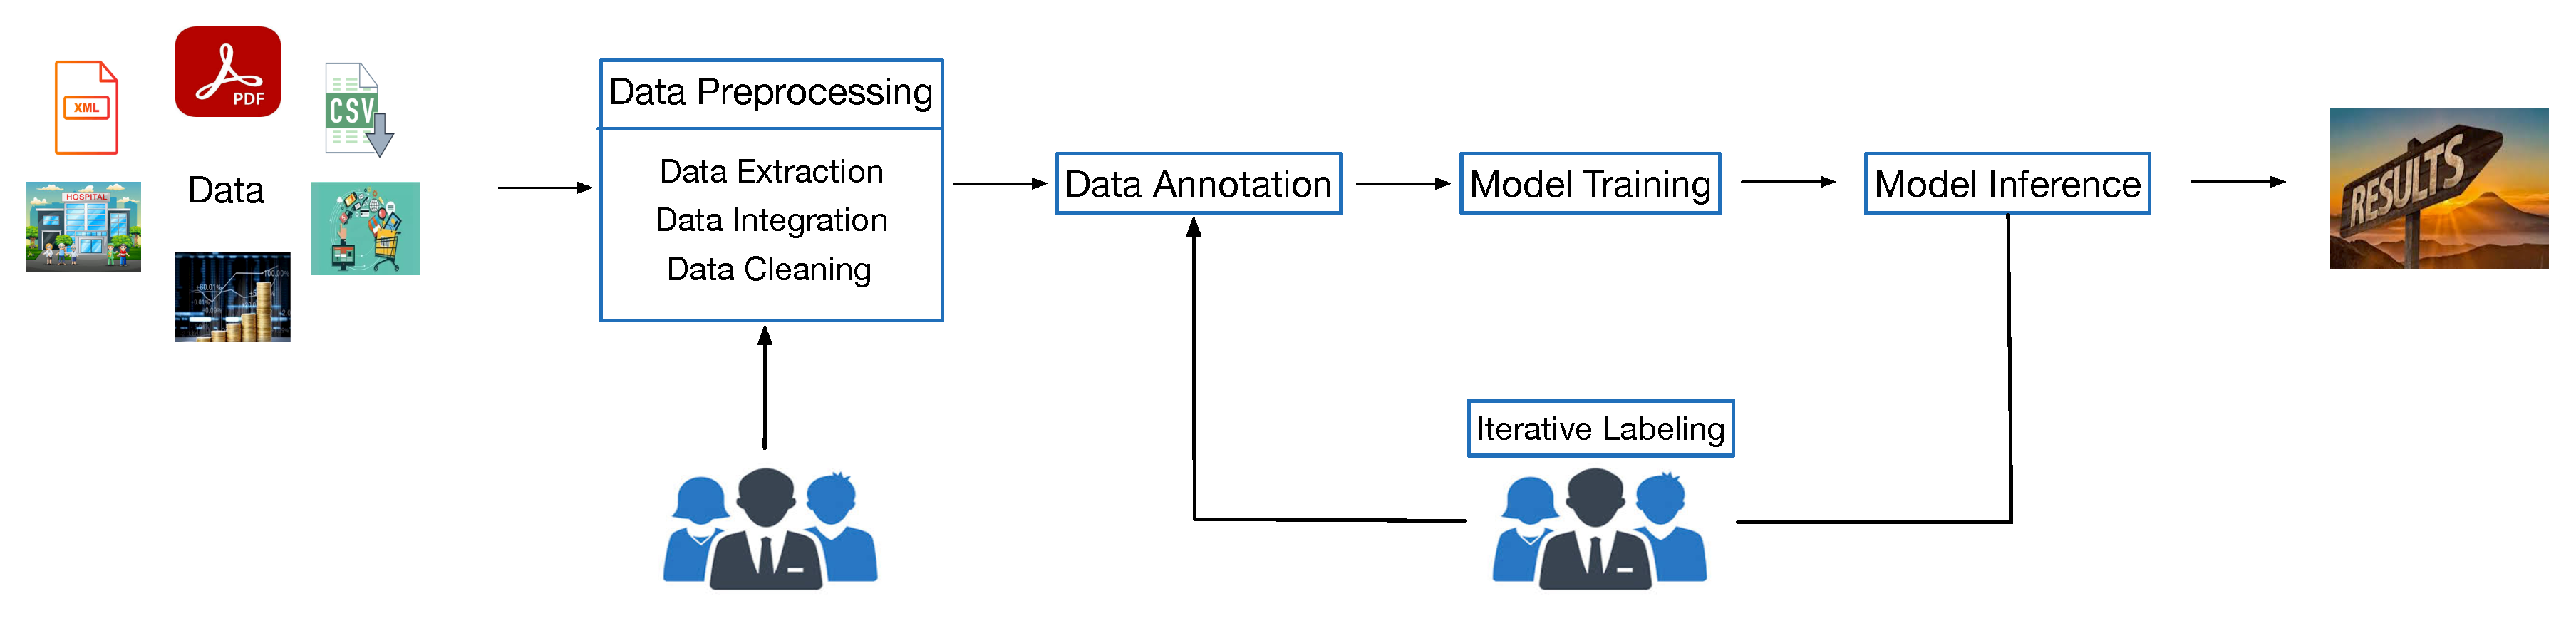
\includegraphics[width=0.65\textwidth]{
%NSFcore-2023/framework.pdf}
 %%\caption{Proposed Project}\label{project}
%\end{wrapfigure}



%We intend to propose complete, partial (either order or unordered), and various qualitative individual preference elicitation models.  An example of the first two would be having complete or only top-$k$ order of preferences over the candidates as inputs, whereas, an example of the last one  would be to bucketize candidates in different qualitative groups (recall the motivating example). For fairness, our effort would be to design group based fairness criteria designed over the protected attributes of the candidates that resemble group fairness criteria, such as, demographic parity, or statistical parity, studied in the context of classification~\cite{verma2018fairness}. To that end, we will adapt proportionate-fairness or p-fairness~\cite{pfair,chairman}  from resource allocation theory that ensures proportionate representation of every group based on a protected attribute in every position of the produced results, or its generalization~\cite{amer2009group} adapted from the social choice theory to promote affirmative action~\cite{fu2006theory} in the produced results.  
%Preference aggregation would be studied considering Kendall-Tau and Spearman's Footrule Distance functions~\cite{kemeny,diaconis1977spearman}, with the objective to minimize the sum of disagreement (Kemeny Optimization) or such, akin to existing {\em (fairness unaware) classical rank aggregation problem}~\cite{dwork2001rank,ailon2008aggregating, ailon2010aggregation}. Our goal would be to make these solutions fairness aware by investigating how to combine these two somewhat conflicting aspects in a systematic manner. For each of these proposed problem variants, we shall analyze the nature of the problem analytically and design scalable solutions with theoretical guarantees. Finally, we will perform both qualitative and quantitative study to develop actionable interventions by leveraging our proposed framework to promote fairness in two compelling applications: (i) Ranked Choice Voting (RCV)~\cite{rcv1,rcv2}, and (ii) Gender and diversity gap in the Oscars. We intend to fine-tune our proposed models based on these evaluations. 

\noindent {\bf Comparison with Existing Work.}
This contribution builds on our work recent works on fairness~\cite{islam2022satisfying, wei2022rank}, and prior works on preference aggregation~\cite{amer2009group, amer2015group, basu2015group}, studying robustness~\cite{roy2014exploiting}. We acknowledge that the existing popular group based fairness definition, such as, {\em statistical parity}~\cite{dwork2012fairness} is somewhat similar to one of our proposed fairness notion. However, the best adapted version of top-$k$ statistical parity studied in a recent paper~\cite{vldbrank} does not account for proportionate representation in every position of the top-$k$, limiting its applicability.  Studying computational challenges related to computing the margin of victory  has been a focus of recent research~\cite{stv1,stv2, stv3} in the context of electoral voting and related applications. But none of these existing works study the general version of the problem, which is, how to promote additional simple/complex constraints/criteria in the output, which is our primary focus. Other than these prior works, which are  much narrow in scope, we are unaware of any computational work that systematically studies different preference elicitation models, multiple output changing criteria, and preference aggregation combining these two.  

%Section~\ref{related} provides an in-depth comparison between our proposed work and existing work.  
%To the best of our knowledge, we are the first to investigate a generic framework that can minimally update original outcome of preference aggregation to satisfy complex constraints without any assumption on the relationship among the attributes.

%Using the aforementioned example, if $k=12$, existing work~\cite{vldbrank} only ensures p-fairness of the aggregated rank at position $12$, but not for the remaining positions (e.g., 1 to 11). {\em While p-fairness promotes stronger notion of fairness, and our proposed framework adapts to top-$k$ statistical parity, existing work does not adapt to our proposed optimization framework}.

%\smallskip \noindent {\bf Aim 1 - Fair Rank Aggregation.}
%We will begin our study in the context of ranking, which is a commonly used method to prioritize  desirable outcomes among a set of candidates and is an essential step in  many high impact applications. Here the members elicit a {\em complete preference order} over the candidates and the goal is to produce an aggregated ranked order over all candidates or produce top-$k$ results that minimize disagreements  among individual preferences. When fairness is studied, our goal would be to ensure fair representation of the candidates based on their one or more protected attributes (such as, gender, race, etc.) in the ranked order. 
%\smallskip \noindent {\bf Aim 2 - Fair Partial and Qualitative Preference Aggregation.}
%In this aim we shall consider scenarios where either qualitative preferences or partial rankings are elicited from the members. 
%We consider three such preferences: (1) top-$t$ ranking, where the input preference is a ranking of the top-$t$ items (candidates), (2) subset selection, where the input preference is an unordered subset of favorite elements, and (3) bucketing, where the input preference is a partition of the elements into three subsets: the ``yes'' set, ``ambivalent'' set, and the ``no'' set.  In our preliminary work, we consider the selection of council members or a committee of $k$ members from $n$ candidates considering the votes of $m$ judges (voters) ({\em ranked choice voting}~\cite{rank1} could be considered as a popular application of that).  The fairness criterion models affirmative action and includes a lower and upper bound on the number of elected candidates, for each value of the protected attributes(s). We intend to study the design choices of different preference elicitation models considering fairness, formalize the optimization problems and analyze them, and design principled solutions with guarantees.

%The mechanism we focus on to aggregate the top-$k$ rankings is {\em Ranked choice voting (RCV)}, and specifically RCV employing a single transferable vote (STV) system~\cite{rcvdesc}.
%We are going to follow the mechanism used in Cambridge MA to elect its city council. 

%\smallskip \noindent {\bf Aim 3 - Actionable Fair Preference Aggregation.}
%Although the proposed models and algorithms consider 
%fairness in its design, rather than an afterthought, the third aim will delve deeper into fairness considerations of compelling applications and develop actionable interventions. In particular, the third aim will provide a holistic large-scale study over two compelling applications and present actionable interventions to promote fairness. In the first application, we will study fairness in Ranked Choice Voting (RCV)\footnote{\small https://qz.com/1676718/the-pros-and-cons-of-ranked-choice-voting/} considering the data provided by the Cambridge, MA
%City Council Election 2019~\cite{RCV} to analytically answer important questions raised in recent research~\cite{rcv1,rcv2,rcv3, rcv4,rcv5}. 1. Does more choice lead to reduced racially polarized voting? 2. Does ranked choice voting enable minority representation?  Based on the analysis, {\em we will develop actionable interventions by leveraging our proposed framework to mitigate these risks}. We will perform both qualitative and quantitative analysis. For qualitative  analysis, we will recruit experienced workers from Amazon Mechanical Turk (the budget justification provided further details). A similar  study would be conducted to investigate the gender and diversity gap in the Academy of Motion Picture Arts and Sciences decisions by combining it with large scale Movielens~\cite{movielens} data and we will develop actionable recommendation to mitigate the gap. Further evaluation plan considering other datasets is described in Section~\ref{eval}.

%\section{Introduction}
\label{seC:intro}
% Interpretability and nutritional labels, generally

An essential ingredient of successful machine-assisted decision-making, particularly in high-stakes decisions, is interpretability --– allowing humans to understand, trust and, if necessary, contest, the computational process and its outcomes.   These decision-making processes are typically complex:  carried out in multiple steps, employing models with many hidden assumptions, and relying on datasets that are often repurposed --- used outside of the original context for which they were intended.\footnote{See Section 1.4 of Salganik's ``Bit by Bit''~\cite{salganik} for a discussion of data repurposing in the Digital Age, which he aptly describes as "mixing readymades with custommades.''}  In response, humans need to be able to determine the ``fitness for use'' of a given model or dataset, and to assess the methodology that was used to produce it.  

To address this need, we propose to develop interpretability and transparency tools based on the concept of a {\em nutritional label}, drawing an analogy to the food industry, where simple, standard labels convey information about the ingredients and production processes. Short of setting up a chemistry lab, the consumer would otherwise have no access to this information. Similarly, consumers of data products cannot be expected to reproduce the computational procedures just to understand fitness for their use.   Nutritional labels, in contrast, are designed to support specific decisions by the consumer rather than completeness of information.  A number of proposals for hand-designed nutritional labels for data, methods, or both have been suggested in the literature\cite{DBLP:journals/corr/abs-1803-09010,DBLP:journals/corr/abs-1805-03677,DBLP:conf/fat/MitchellWZBVHSR19}; we advocate deriving such labels automatically or semi-automatically as a side effect of the computational process itself, embodying the paradigm of {\em interpretability-by-design}. 

Interpretability means different things to different stakeholders, including individuals being affected by decisions, individuals making decisions with the help of machines, policy makers, regulators, auditors, vendors, data scientists who develop and deploy the systems, and members of the general public.  Designers of nutritional labels must therefore consider {\em what} they are explaining,  {\em to whom}, and {\em for what purpose}.  In the remainder of this section, we will briefly describe two regulatory frameworks that mandate interpretability of data collection and processing to members of the general public, auditors, and regulators,  where nutritional labels offer a compelling solution (Section~\ref{sec:intro:reg}).  We then discuss interpretability requirements in data sharing, particularly when data is altered to protect privacy or mitigate bias (Section~\ref{sec:intro:synth}).

\subsection{Regulatory Requirements for Interpretability}
\label{sec:intro:reg}

The European Union recently enacted a sweeping regulatory framework known as the General Data Protection Regulation, or the GDPR~\cite{gdpr}.  The regulation was adopted in April 2016, and became enforceable about two years later, on May 25, 2018.  The GDPR aims to protect the rights and freedoms of natural persons with regard to how their personal data is processed, moved, and exchanged (Article 1).  The GDPR is broad in scope, and applies to ``the processing of personal data wholly or partly by automated means'' (Article 2), both in the private sector and in the public sector.  Personal data is broadly construed, and refers to any information relating to an identified or identifiable natural person, called the {\em data subject} (Article 4).  

According to Article 4, lawful processing of data is predicated on the data subject's {\em informed consent}, stating whether their personal data can be used, and for what purpose (Articles 6, 7).
Further,  data subjects have {\em the right to be informed} about the collection and use of their data.~\footnote{\url{https://gdpr-info.eu/issues/right-to-be-informed/}}
Providing insight to data subjects about the collection and use of their data requires technical methods  that support interpretability.  

Regulatory frameworks that mandate interpretability are also starting to emerge in the US.  New York City was the first US municipality to pass a law (Local Law 49 of 2018)~\cite{Vacca}, requiring that a task force be put in place to survey the current use of ``automated decision systems'' (ADS) in city agencies. ADS are defined as ``computerized implementations of algorithms, including those derived from machine learning or other data processing or artificial intelligence techniques, which are used to make or assist in making decisions.''   The task force is developing recommendations for enacting algorithmic transparency by the agencies, and will propose procedures for: (i) requesting and receiving an explanation of an algorithmic decision affecting an individual (Section 3 (b) of Local Law 49); (ii) interrogating ADS for bias and discrimination against members of legally protected groups, and addressing instances in which a person is harmed based on membership in such groups (Sections 3 (c) and (d)); (iii) and assessing how ADS function and are used, and archiving the systems together with the data they use (Sections 3 (e) and (f)).

Other government entities in the US are following suit.  Vermont is convening an Artificial Intelligence Task Force to ``... make recommendations on the responsible growth of Vermont’s emerging technology markets, the use of artificial intelligence in State government, and State regulation of the artificial intelligence field.''~\cite{Vermont}.  Idaho’s legislature has passed a law that eliminates trade secret protections for algorithmic systems used in criminal justice~\cite{Idaho}.  In early April 2019, Senators Booker and Wyden introduced the Algorithmic Accountability Act of 2019 to the US Congress~\cite{BookerWydenClarke}. The Act, if passed, would use ``automated decision systems impact assessment'' to address and remedy harms caused by algorithmic systems to federally protected classes of people. The act empowers the Federal Trade Commission to issue regulations requiring larger companies to conduct impact assessments of their algorithmic systems.

The use of nutritional labels in response to these and similar regulatory requirements can benefit a variety of stakeholders.  The designer of a data-driven algorithmic method may use them to validate assumptions, check legal compliance, and tune parameters.  Government agencies may exchange labels to coordinate service delivery, for example when working to address the opioid epidemic, where  at least three sectors must coordinate: health care, criminal justice, and emergency housing, implying a global optimization problem to assign resources to patients effectively, fairly and transparently. The general public may review labels to hold agencies accountable to their commitment to equitable resource distribution. 


\subsection{Interpretability with Semi-synthetic Data}
\label{sec:intro:synth}

%Datasets are now increasingly used to train models to make decisions once made by humans.  In these automated systems, biases in the data are propagated and amplified with no human in the loop.  The bias, and the effect of the bias on the quality of decisions made, is not easily detectable due to the relative opacity of the system.  

A central issue in machine-assisted decision-making is its reliance on historical data, which often embeds results of historical discrimination, also known as {\em structural bias}.   As we have seen time and time again, models trained on data will appear to work well, but will silently and dangerously reinforce discrimination~\cite{propublicaJ,amazon_hiring,amazon_delivery}.  Worse yet, these models will legitimize the bias --- ``the computer said so.''  Nutritional labels for data and models are designed specifically to mitigate the harms implied by these scenarios, in contrast to the more general concept of ``data about data.''

Good datasets drive research: they inform new methods, focus attention on important problems, promote a culture of reproducibility, and facilitate communication across discipline boundaries.  But research-ready datasets are scarce due to the high potential for misuse. Researchers, analysts, and practitioners therefore too often find themselves compelled to use the data they have on hand rather than the data they would (or should) like to use.  For example, aggregate usage patterns of ride hailing services may overestimate demand in early-adopter (\ie wealthy) neighborhoods, creating a feedback loop that reduces service in poorer neighborhoods, which in turn reduces usage.  In this example, and in many others, there is a need to alter the input dataset to achieve specific properties in the output, while preserving all other relevant properties.  We refer to such altered datasets as \textit{semi-synthetic}.

Recent examples of methods that produce semi-synthetic data include database repair for causal fairness~\cite{DBLP:conf/sigmod/SalimiRHS19}, database augmentation for coverage enhancement~\cite{DBLP:conf/icde/AsudehJJ19}, and privacy-preserving and bias-correcting data release~\cite{DBLP:conf/ssdbm/PingSH17,DBLP:conf/vldb/RodriguezSPSH18}. A semi-synthetic datasets may be altered in different ways.  Noise may be added to it to protect privacy, or statistical bias may be removed or deliberately introduced.  When a dataset of this kind is released, its composition and the process by which it was derived must be made interpretable to a data scientist, helping determine fitness for use.  For example, datasets repaired for racial bias are unsuitable for studying discrimination mitigation methods, while datasets with bias deliberately introduced are less appropriate for research unrelated to fairness.   This gives another compelling use case for nutritional labels.

%To make our discussion more concrete, let us consider data scientists who must identify datasets appropriate for their task.  This is particularly important when semi-synthetic datasets are being released, to which noise is added to protect privacy, or statistical bias is removed or deliberately introduced.  For example, datasets repaired for racial bias are unsuitable for studying discrimination mitigation methods, while datasets with bias deliberately introduced are less appropriate for research unrelated to fairness.  



%\input{IEEE-data-engineering-IC1/preliminary}
\vspace{-0.2in}
\section{Formalism}\label{preliminary}
\vspace{-0.1in}
%The proposed work aims at developing an optimization guided computational framework that modifies an output obtained from a preference aggregation method applied on a preference elicitation model to produce a modified output that satisfies given criteria. The proposed work aims at developing this framework for a suite of preference elicitation models and preference aggregation methods.
%that satisfies with criteria that guides the need to change the original output minimally while producing a complete or top-$k$ (ordered or unordered) result aggregating individual preferences.

There are $4$ types of inputs that our proposed framework takes: (a)~a set $N$ of $n$ items, where each item has a set $\mathcal{A}$ of discrete attributes.  Each attribute $a\in \mathcal{A}$ has $\ell_a$ different values. (b)~a set of $m$ users, where the $i$-th user $u(i)$ provides her preference as $\sigma_i$. The users' preferences could be rank based, partial or full order, or non rank based. (c)~a distance function $\mathcal{F}$ (defined formally below) that measure the ``distance'' between a set of $m$ input preferences  $\sigma_1, \sigma_2,\ldots, \sigma_m$ and an output $\sigma$ with the required output form. The exact distance function depends on the underlying preference elicitation model and the required output form which may be either a complete ranking of the items or a subset of $k$ items, either ranked or not. (d)~a set $\mathcal{C}$ of output criteria/constraints. Some variants of our problem also include as input a budgetary constraint $B$.

%The proposed work aims at developing an optimization guided computational framework that suitably combines a suite of preference elicitation models with criteria that guides the need to change the original output minimally while producing a complete or top-$k$ (ordered or unordered) result aggregating individual preferences. %Next, we present some definitions that will be used throughout the proposal.  

\begin{definition}\label{def4}
\vspace{-0.1in}
{\bf Distance function $\mathcal{F}$.} Given $m$ input preferences  $\sigma_1, \sigma_2,\ldots, \sigma_m$ and an output $\sigma$ with the required output form, the function $\mathcal{F}(\sigma, \sigma_1, \sigma_2,\ldots, \sigma_m)$ is the distance of $\sigma$ from the input preferences  $\sigma_1, \sigma_2,\ldots, \sigma_m$.
In some cases the function $\mathcal{F}(\cdot)$ is an aggregation of a distance function between a single input preference and the output. Examples for such an aggregation are the sum of the pairwise distances and the maximum distance to any of the input preferences. In other cases $\mathcal{F}(\cdot)$ measures the minimum modification of the input preferences that would result in the preference aggregation method outputting the output $\sigma$. 
%$\mathcal{F}(\sigma, [\sigma_1, \sigma_2,\ldots, \sigma_m])$
\end{definition}

\vspace{-0.1in}
\begin{definition}\label{def1}
\vspace{-0.1in}
{\bf Output criteria/constraints.}  For an attribute $a\in \mathcal{A}$,  let $c(p_a)$ denote the cardinality constraints of items with value $p_a$ ($p_a$ is one of the $\ell_a$ possible values of attribute $a$). Given to the framework is a set $C$ of such cardinality constraints for each attribute value $p_a$, for every $a \in A$, $A \subset \mathcal{A}$. There are two explicit cases that we consider.
\begin{itemize}
    \item {\bf The output $\sigma$ is ordered and consists of $k\le n$ items.} 
    In this case the cardinality constraints are defined for every $\kappa \in [1..k]$ items, and for every  such $\kappa \in [1..k]$, the $\kappa$ top ranked items of output $\sigma$ have to satisfy these cardinality constraints.  
    %the $k$ top ranked items satisfy all cardinality constraints defined over $v$, i.e., it satisfies $c(p^v_{a_1}) \text{ AND } c(p^v_{a_2}) \text{ AND } \ldots \text{ AND } c(p^v_{a_A})$.  
     \item {\bf The output $\sigma$ is an unordered set of $k$ items.} In this case the cardinality constraints are defined for $k$ items and the items in the output set $\sigma$ have to satisfy these cardinality constraints. 
     \\ %$c(p_{a_1}) \text{ AND } c(p_{a_2}) \text{ AND }  \ldots \text{ AND } c(p_{a_A})$.  
\end{itemize}  
\end{definition}
\vspace{-0.1in}
\begin{definition}\label{def3}
\vspace{-0.1in}
{\bf A budgetary constraint.} A budgetary constraint $B$ is an upper bound on the distance of the output from the input preferences. 
%For a given distance function $\mathcal{F}(\cdot)$, 
The budgetary constraint implies that $\mathcal{F}(\sigma,\sigma_1,\sigma_2,\ldots,\sigma_m)\leq B$.  
\end{definition}

\vspace{-0.1in}
\begin{definition}\label{def2}
{\bf Preference Aggregation Considering Constraints.} 
We intend to study different types of problem definitions that require different algorithmic treatments.
Given either complete or partial preferences $\sigma_1,\sigma_2,\ldots,\sigma_m$ over the items in $N$, a preference aggregation method, a distance function $\mathcal{F}(\cdot)$, and a set of output criteria $\mathcal{C}$.
\vspace{-0.1in}
\begin{itemize}
    \item {\bf (Constrained optimization).} Produce an output $\sigma$ with the required form that minimizes $\mathcal{F}(\sigma,\sigma_1,\sigma_2,\ldots,\sigma_m)$ and satisfies $\mathcal{C}$.
    \vspace{-0.1in}
    \item {\bf (Optimization under budgetary constraints).} Produce an output $\sigma$ with the required form that optimizes $\mathcal{C}$,  while satisfying $\mathcal{F}(\sigma,\sigma_1,\sigma_2,\ldots,\sigma_m) \leq B$. (The objective function for optimizing $\mathcal{C}$ varies.)
    \vspace{-0.1in}
    \item {\bf (Bi-criteria optimization).} Given parameters $\alpha$ and $\beta$ produce an output $\sigma$ with the required form that satisfies both $\mathcal{F}(\sigma,\sigma_1,\ldots,\sigma_m) \le \alpha$ and $\mathcal{G}(\mathcal{C}) \le \beta$, where $\mathcal{G}$ is the objective function for optimizing $\mathcal{C}$.
\end{itemize}
\end{definition}
%The individual research aims will describe the various forms of preference elicitation from users and the details of the preference aggregation methods. We first delineate the need to change original output and the challenges that arise from there.
\vspace{-0.1in}
\subsection{Specifying Output Criteria}
We discuss orthogonal reasons where the original outputs coming out of the preference aggregation methods need to be ``massaged'' further. What unifies them is that these criteria are defined over one or more attributes of the items. Depending on how many attributes are involved in the definition and their relationship thereof gives rise to additional challenges.


%\vspace{-0.1in}
%\subsection{Important Concepts and Definitions}\label{pre}
%\vspace{-0.1in}
%\noindent \textbf{Database.} contains $n$ items or candidates. These two terms will be used interchangeably. The set of items will be denoted $V$, individual items will be denoted by $u$ and $v$. \\
%\noindent {\em \bf Individual preference Elicitation:} We consider the following individual preference elicitation models. \\
%\noindent (1) Complete preference: Each of the $4$ members (Judges) may provide a {\em complete order of preference} over the $12$ candidates (Refer to Table~\ref{tab:example_original_rank}). \\
%\noindent (2) Partial preference: 
%(2.1) Ordered. Member 1 (as well as other members) may provide a partial order over the first $5$ candidates and does not specify anything for the rest.\\
%(2.2) Unordered. Member 1 (as well as other members) may also specify that she likes the first $5$ candidates without specifying any order among them.\\
%\noindent (3) Qualitative Preference: Contrarily, Member 1 (as well as other members) may provide {\em qualitative preferences}: Molly and Amy are preferred, Abigail, Kim, Lee are acceptable, the remaining ones must not be considered. These are considered to be the inputs to the framework. Please note that 2.2 is a simplified variant of this last preference elicitation model.

%\noindent \textbf{Multiple Preferences.} The input consists $m$ different preference elicitation (based on the individual models described above). Using the motivating example, $m=4$.

\subsubsection{Fair Preference Aggregation}
We will study fairness in the context of group based protected attributes of the candidates. Output criteria/constraints for fairness (refer to Definition~\ref{def1}) are expressed over one or more {\em protected attributes}. Their protected attributes could be expressed over gender, ethnicity, race, or the state the candidates are living in. 

Formally speaking, each item/candidate $v\in N$ has one or more  {\em protected attributes}. When $\ell_a=2$, it is a binary protected attribute; when $\ell_a \geq 2$ it is a multi-valued protected attribute. As an example, race is (usually) a multi-valued protected attribute, and gender is sometimes a binary protected attribute.

%\begin{itemize}
%\item  {\bf p-fairness.} 
\smallskip \noindent \textbf{p-fairness.}
p-fairness has been studied in the context of resource allocation satisfying temporal fairness or proportionate progress~\cite{chairman, pfair}. It was introduced in the classical  {\em Chairman Assignment Problem}~\cite{baayen1964existence, chairman} that studies how to select a chairman of an union every year from a set of  $n$ states such that  that at any time the accumulated number of chairmen from each state is proportional to its weight. 

In the context of ranking, suppose that each of the $n$ ranked items has a {\em protected attribute} $a(\cdot)$ that can take any of $\ell_a$ different values. For $p_a\in [1..\ell_a]$, let $c'(p_a)$ denote the fraction of items with protected attribute value $p_a$, that is, $c'(p_a) = \frac 1n \sum_{i=1}^n \bbone_{a(i)=p_a}$. The goal is to ensure that $c'(p_a)$ fraction (rounded either up or down) of every top $\kappa$ items have protected attribute value $p_a$.
\iffalse
\vspace{-0.1in}
\item {\bf Generalization of p-fairness to promote affirmative action.} Instead of requiring $c'(p_a)$ fraction of every top $\kappa$ items to have protected attribute value $p_a$, we may want that certain values of the protected attribute get higher representation among the elements at the top, more than their overall proportion. Let $P$ be a non-negative doubly stochastic $n \cdot \ell_a$ matrix. The goal is to ensure that $P(\kappa,p_a)$ fractions (rounded either up or down) of the top $\kappa$ items to have value $p_a$, for every $\kappa \in [1..n]$ and $p_a\in [1..\ell_a]$ (if it is feasible).
It is not difficult to note that such a generalized notion can capture affirmative action.
%\end{itemize}
\fi


\subsubsection{Robust Preference Aggregation}
Output criteria/constraints for robustness on the other hand investigates the flip questions: Given either complete or partial preferences $\sigma_1,\sigma_2,\ldots,\sigma_m$ over $n$ items, let $\sigma$ be the output obtained by the preference aggregation method. Given a budget $B$, how to  make $B$ or less changes in the original preferences, such that the outcome is different from $\sigma$? This question is  related to finding the {\em margin} in electoral systems and quantifies how manipulable the underlying aggregation method is. We study this problem under different manipulation models -- addition only, deletion only, or substitution (addition + deletion).

\iffalse
\subsection{Challenges in Handling  Complex Output  Criteria}
In general, the output requirements/constraints are defined over a set $R$ of attributes. When $|R|=1$, as an example, the output requirement is defined on a single attribute (such as race). In a recent work, we demonstrated that for an aggregation method that models plurality voting, the problem of preference aggregation while satisfying output criteria defined by a single attribute is computationally easy. 
However, the nature of the problem changes when two or more attributes are involved in the output criteria. In Section~\ref{aim1} we discuss this more complicated case and refer to our recent work in which we showed evidence that in some cases it is computationally difficult even to find any output with the required form. 
\fi
%When there are two or more different attributes involved in outlining output criteria/constraints (such as certain representation from race and certain representation from gender), the PIs have proved in a recent work~\cite{islam2022satisfying} that the decision version of the preference aggregation problem under output constraint becomes (weakly) NP-hard by reducing the well known NP-hard Partition problem to our problem~\cite{garey1979computers}. We note that the existing practice of converting multiple attributes to a single multi-valued protected attribute by computing joint distribution over the attributes assumes independence among the attributes. When Independence among the attributes does not hold, this simplification leads to a heuristic process.  The PIs have also demonstrated that for three (or more) attributes (e.g., constraints defined over race, and gender, and ethnicity), even the question whether there exists a set of top-$k$ that satisfies the complex constraint is strongly NP-Hard where the reduction is fro 3 Dimensional Matching. On the positive side for the case of two  attributes, the PIs have designed an efficient algorithm a preference aggregation algorithm while satisfying fairness constraints defined over $2$ attributes and has designed a 2 approximation factor and runs in $O(n^2\ell \log m)$ time, by casting this problem as a min cost flow problem, where $\ell$ is the total number of possible attribute values. We intend to study these aspects in the proposal - as it turns out to be an intellectually demanding and independent  facet of the computational problem, irrespective of the specific reasons to change the output.


%\input{IEEE-data-engineering-IC1/aim1}
\vspace{-0.2in}
\section{Single Round Rank based Preference Aggregation}\label{aim1}
\vspace{-0.1in}
We outline two separate lines of algorithmic problems: (1) incorporating output criteria (e.g., p-fairness) in single round rank-based preference aggregation methods, and (2) satisfying complex constraints in single round rank-based preference aggregation methods.
\vspace{-0.1in}
\subsection{Incorporating output criteria in rank aggregation} 
\vspace{-0.1in}
The input to the classical {\em rank aggregation} problem consists of $m$ complete order of preferences over the $n$ items/candidates. Traditionally, producing the final ranking involves aggregating potentially conflicting preferences from multiple individuals, and is known as the rank aggregation problem~\cite{dwork2001rank,van2007deterministic, ailon2008aggregating}. Our goal is to  minimally change the aggregated output to enable fairness.
%p-fairness has been studied in the theory community to enable resource allocation satisfying temporal fairness or proportionate progress.
We will study p-fairness~\cite{chairman, pfair} that ensures proportionate representation of every group based on a protected attribute in every position of the aggregated ranked order.  The classical problem in this context is known as the {\em Chairman Assignment Problem}~\cite{baayen1964existence, chairman} which studies how to select a chairman of a union every year from a set of  $r$ states such that  that at any time the accumulated number of chairmen from each state is proportional to its weight. p-fairness generalizes other notions of fairness~\cite{islam2023equitable} that were considered in prior work, including the existing popular group based fairness definition {\em statistical parity}~\cite{dwork2012fairness}. 
%We start with some definitions and then describe both our preliminary research and the open problems we plan to investigate further.
\vspace{-0.1in}
\subsubsection{Research Directions}
\vspace{-0.1in}
%\noindent \textbf{Rank and Multiple Ranking.}  
Consider rankings of the items in a set $V$. Each such ranking can be viewed as a permutation. We will use the terms ranking and permutation interchangeably. 

\noindent \textbf{Kendall-Tau and Kemeny distances.}
	Given two rankings $\sigma,\eta: V \rightarrow [1..n]$, the
	Kendall-Tau distance between the two rankings is the sum of pairwise disagreements between $\sigma$ and $\eta$ (bubble-sort distance)
	\[
	\cK (\sigma,\eta) = \sum_{\{u,v\}\subseteq V} \bbone_{(\sigma(v)-\sigma(u))(\eta(v)-\eta(u))<0}.
	\]
	
	For a set of rankings
	$\{\eta_1,\eta_2,\ldots,\eta_m\}$ the {\em Kemeny distance} of the ranking
	$\sigma$ to this set as
	\[
	\kappa(\sigma,\eta_1,\eta_2,\ldots,\eta_m)= \sum_{i=1}^m \cK (\sigma,\eta_i).
	\]

 \noindent \textbf{Spearman's footrule distance.}
    Given two rankings $\sigma,\eta: V \rightarrow [1..n]$, the 	Spearman's footrule distance between the two rankings is the sum of the absolute values
  ($\ell_1$ distance) of the differences between rankings $\sigma$ and $\eta$.
	\[
	\cS (\sigma,\eta) = \sum_{u\in V} |(\sigma(u)-\eta(u)|
	\]
 
	For a set of rankings
	$\{\eta_1,\eta_2,\ldots,\eta_m\}$ the {\em Spearman's footrule distance} of the ranking
	$\sigma$ to this set is the sum of the pairwise distances.

    \noindent \textbf{Rank aggregation.} The aggregated ranking of a set of $m$ rankings $\{\rho_1,\rho_2,\ldots,\rho_m\}$ for a given distance function is a ranking that minimizes  the distance to this set.
    
    \noindent \textbf{p-fairness for a ranking.}
    For a permutation $\sigma, k\in [1..n], p\in [1..\ell]$, let $P(\sigma,k,p)$ denote
    the number of elements with protected attribute value $p$ among the $k$ top ranked elements
    in $\sigma$. A ranking $\sigma$ is {\em proportionate fair} or {\em p-fair} if
    \[
    \forall k\in [1..n]\, \forall p\in [1..\ell]:\  P(\sigma,k,p)\in \{\floor{f(p)\cdot k},\ceil{f(p)\cdot k}\}.
    \]

 
%We note that the best adapted version of top-$k$ statistical parity studied in a recent paper~\cite{vldbrank} does not account for proportionate representation in every position in the top-$k$ positions, but just to a small number of positions, thus limiting its applicability.
%As a matter of fact it can be shown that the algorithm Fair-ILP presented in~\cite{vldbrank} for the special case of a binary protected attribute in which the frequency of both values is the same may produce a very skewed output. This is because the algorithm Fair-ILP just considers the {\em total number of times} items with one value of protected attribute are ranked above items with the other value. p-fairness is  stronger because it ensures statistical parity for every position in the ranked order and considers, for every $k$, the number of times items in the top-$k$ with one value of protected attribute are ranked above items with the other value. This makes this notion of fairness significantly harder to implement and the existing solutions do not trivially adapt.


We formalized two optimization problems, individual p-fairness or {\bf IPF} and the rank aggregation problem subject to proportionate fairness ({\bf RAPF})  considering binary ($\ell=2$) and multi-valued ($\ell > 2$) protected attributes. These problems and associated algorithmic results could be found in~\cite{wei2022rank}.


\vspace{-0.1in}
\subsubsection{Open Problems}
\vspace{-0.1in}
We plan to investigate the following open problems.

\smallskip \noindent{\bf p-fairest aggregate ranking (PFAR).} 
The PFAR problem is defined as follows. Given a set of $m$ rankings %$\{\rho_1,\rho_2,\ldots,\rho_m\}$ 
choose the ``p-fairest'' ranking among all rankings that minimize the Kemeny distance to this set. 
We need to define ``p-fairest'' ranking or a distance measure to a p-fair ranking.
We propose the following distance measure (using the notations defined above).
For an integer $d \ge 0$, a ranking $\sigma$ is at distance $d$ from a {\em p-fair} ranking if
\[
\forall k\in [1..n]\, \forall p\in [1..\ell]:\  P(\sigma,k,p)\in \{\floor{f(p)\cdot k}-d,\ceil{f(p)\cdot k}+d\}.
\]

\iffalse
Another way to view the distance to a p-fair ranking is by considering the classical {\em p-processor cup game} defined by Liu~\cite{liu1969} that considered the notion of p-fairness in multi processor scheduling. The p-processor cup game (adapted to our case) is a multi-round game with two players, an {\em emptier} and a {\em filler}, that takes place on $\ell$ cups, each filled initially with a fixed amount of water, called {\em buffer}. At the beginning of each round,
the filler adds a total of 1 gallon of water to the cups. The distribution of this 1 gallon to the cups is determined by the filler.
The emptier then selects a single cup (that must have at least 1 gallon of water)
and removes 1 gallon from this cup. The emptier’s goal is to minimize the size of the buffer and the {\em backlog} which is the amount of water (on top of the initial amount) in the fullest cup.

It is easy to see the analogy to p-fairness. Consider a p-fair ranking of $n$ elements each with a protected attribute with $\ell$ possible values. Each cup represents a possible value of the protected attribute. The corresponding game has $n$ rounds. In each round $k\in [1..n]$ the filler
adds $f(p)$ gallons of water to cup $p$, for $p\in [1..\ell]$, and the emptier removes 1 gallon of water from the cup corresponding to the value of the protected attribute of the element ranked $k$.
The existence of a p-fair ranking implies that the emptier can always guarantee that the size of the buffer and the backlog is no more than 1 gallon.
For a ranking that is at distance $d$ from a p-fair ranking, the emptier can guarantee that the size of the buffer and the backlog is no more than $1+d$ gallons.
\fi

We observe that PFAR is also NP-Hard as directly follows from the fact that unconstrained rank aggregation is NP-hard when 
$m\ge 4$~\cite{ailon2008aggregating}. For some fixed $\alpha > 1$, We would like to find an algorithm that finds the p-fairest ranking among all rankings whose Kemeny distance from the set of input rankings is at most $\alpha$ times the minimum such distance. 
%Reasonable values of $\alpha$ to consider are 
%$\frac 85$ and $\frac 43$ since there are efficient $\frac 85$ and $\frac 43$ approximation algorithm for the rank aggregation problem~\cite{ailon2008aggregating}.

\smallskip \noindent {\bf Bi-criteria p-fair rank aggregation (BPFRA).} 
The most general problem that we plan to consider in this context is the bi-criteria optimization problem, that is, for a given pair $(\alpha>1 ,\beta>1)$ and a set of $m$ rankings %$\{\rho_1,\rho_2,\ldots,\rho_m\}$
find a ranking whose Kemeny distance to the set of rankings is at most $\alpha$ times the Kemeny distance of the aggregated rank from the set and its distance from a p-fair ranking is at most $\beta$, if such a ranking exists.

\smallskip \noindent{\bf p-fair rank aggregation with affirmative action.} 
We plan to consider a variant of p-fair rank aggregation that involves ``affirmative action''. This will be modeled by varying the proportion of the values of the protected attribute in the p-fair aggregated rank. For example, consider a binary protected attribute with values A and B each needs to appear the same number of times. Suppose that our goal is to promote the items with attribute value A. In this case we can vary the proportion of A making it higher in the top ranked elements and lower in the lower ranked elements so that overall items with attribute value A will appear the same number of times as items with attribute value B.

\smallskip \noindent{\bf The complexity of individual p-fair ranking (IPF).}  We plan to further investigate the IPF problem for multi valued protected attributes as it is open whether it can be solved accurately in polynomial time. We conjecture that this problem is NP-Hard. %and plan to look for a suitable reduction to prove this conjecture. 
We also plan to look for improved approximation algorithms for this problem.
%We note that the algorithm DetConstSort given in~\cite{kddrank} does not produce closest ranking to a given input ranking.

\smallskip \noindent {\bf Better approximation of rank aggregation subject to p-fairness (RAPF).}
We plan to develop more sophisticated RAPF algorithms with better approximation ratios,  %One approach for designing such algorithms is to apply the pivoting technique presented in~\cite{ailon2008aggregating} for rank aggregation. We also plan 
and to improve the computational aspects of the RAPF problem. This problem can be formulated as an Integer Programming (IP) problem. %and thus the RAPF problem of reasonable size can be solved in practice using an IP solver like Gurobi or CPLEX.
We plan to consider various IP formulations as well as various rounding techniques to accelerate the computation.

\smallskip \noindent{\bf Robust rank aggregation.} It is known that rank aggregation under Kemeny distance is NP-hard. We will explore other aggregation methods, such as Spearman's footrule and Borda, and study how manipulable these rank aggregation methods are -- that is, if only $x\%$ of the preferences are allowed to be changed, how easy it is to change the outcome.
\vspace{-0.1in}
\subsection{Complex Constraints} 
\vspace{-0.1in}
Our goal is to optimize preference substitution to satisfy complex top-$k$ fairness constraints, where the fairness requirement is defined over a set $R$ of protected attributes. One of the objectives we will consider is {\em minimizing the number of single ballot (ranking) substitutions that guarantee fairness in the top-$k$ results.} 
%In voting theory~\cite{cary2011estimating}, the concept of margin of victory (MOV) is designed to measure electoral competitiveness of the candidates. 
In a preliminary work we defined the problem of finding the smallest number of single ballot substitutions to promote a set of $k$ candidates that satisfy fairness requirements defined over a set $R$ of protected attributes to the top-$k$. 
\vspace{-0.1in}
\subsubsection{Research Directions}
\vspace{-0.1in}
We assume that there are $\ell$ protected attributes , denoted $A_1,\dots, A_\ell$. For $i\in [1..\ell]$, attribute $A_i$ has $\ell_i$ possible values, denoted $A[i,j]$, for $j\in [1..\ell_i]$. Each candidate is associated with a specific value from each attribute.
In addition, we are given target quantities $a[i,j]$, for $i\in [1..\ell]$, and  $j\in [1..\ell_i]$, with property that all row marginals sum to $k$. Namely, for every $i\in [1..\ell]$, $\sum_{j=1}^{\ell_i} a[i,j] = k$. A fair outcome should satisfy the fairness  condition that for $i\in [1..\ell]$, and  $j\in [1..\ell_i]$, exactly $a[i,j]$ candidates whose $A_i$ attribute value is $A[i,j]$ are elected. 

\noindent We note that one way to approach this problem is by converting the multiple protected attributes to a single multi-valued protected attribute by computing joint distribution over the attributes assuming their independence. For example, instead of considering two binary valued attributes $A_1$ and $A_2$ we consider a single attribute with 4 possible values and the requirement that the value $i*j$ should appear $a[1,i]\cdot a[2,j]/k$ times, for $i,j\in \{1,2\}$. The shortcomings of this approach are two-fold: First, this approach may yield that the problem is infeasible while there is still a solution without assuming independence. A solution that assumes independence may be inferior (require more substitutions) than a solution that does not assume independence.

\noindent In~\cite{islam2022satisfying}, we showed that the problem of finding the smallest number of single ballot substitutions (original preference) to promote a set of $k$ candidates that satisfy proportionate representation over a single protected attribute is computationally easy for any domain size of the protected attribute. On the other hand the same problem becomes computationally hard if we increase the number of protected attributes. When there are two different protected attributes involved in outlining the fairness requirement, we proved that the decision version of that problem is (weakly) NP-hard, %by reducing the well known NP-hard Partition problem to our problem~\cite{garey1979computers}. 
For three (or more) protected attribute, even the question whether there exists a set of top-$k$ that satisfies the complex fairness constraint is strongly NP-Hard by a reduction from 3 Dimensional Matching. On the positive side for the case of two protected attributes we designed an efficient algorithm that obtains a 2 approximation factor and runs in $O(n^2\ell \log m)$ time, 
%by casting this problem as a min cost flow problem, 
where $\ell$ is the number of possible attribute values. We also designed an exact algorithm with running time $n^c$, where $c$ is the size of the Cartesian product of all the attribute domains.

\vspace{-0.1in}
\subsubsection{Open Problems}
\vspace{-0.1in}
There propose two possible ways to extend these problems.

\smallskip \noindent {\bf Improved approximation ratio in the case of 2 protected attributes.} 
Since  the problem of minimizing the number of single ballot substitutions in the case of 2 attributes is currently proven to be weakly NP-Hard, it may admit a PTAS (Polynomial Time Approximation Scheme). We plan to investigate the existence of a better approximation algorithm. Alternatively, we will try to improve the hardness result and show that this problem is strongly NP-Hard or Max-SNP Complete. 

\smallskip \noindent {\bf Relaxed solutions in the case of 3 or more protected attributes.} 
Clearly, the hardness result of even checking the existence of a solution in case of 3 or more attributes precludes the existence of any approximation algorithm for this case. We plan to design an algorithm that will generate a relaxed set of items/candidates. The relaxation may be in two dimensions: (i) the generated set will be a top-$k$ set of candidates but the fairness requirements will not be fully satisfied for all protected attributes. (ii) the generated set will have size larger than $k$ but it will satisfy the (lower bounds of the) fairness constraints for top $k$. Clearly, the larger the generated set is the easier the problem. We will find the smallest such extended set that guarantees the fairness  constraints imposed by all protected attributes.


%\input{IEEE-data-engineering-IC1/Aim2}
\vspace{-0.1in}
\section{Multi Round Rank based Preference Aggregation}\label{aim2}
\vspace{-0.1in}
We study algorithmic challenges to satisfy  output constraints in multi-round rank based preference aggregation methods, popularly known as ranked choice voting or (RCV)~\cite{irv1}. 
\vspace{-0.1in}
\subsection{Research Directions}
\vspace{-0.1in}
We start by describing the STV (single transferable vote) method~\cite{stv-irv, stv1} that generalizes the IRV method, and selects a set of $k$ items/candidates as the winners. STV is gaining popularity as an electoral system. It is used to elect candidates to the Australian Senate, in all elections in Malta, in most elections in the Republic of Ireland, and in Cambridge, MA. There are also plans to use STV in other USA localities. As mentioned in Section~\ref{preliminary} this method of preference aggregation is also applicable in other settings.

The input to an STV preference aggregation method consists of $m$ either complete or partial rankings of the items/candidates. Suppose that the total number of items/candidates is $n$ out of which $k$ items need to be elected. The preference aggregation process requires a predefined {\em quota}. In most cases this quota is Droop quota~\cite{droop} defined as $\floor{\frac{n}{k+1}}+1$. The aggregation is done in rounds. In each round every item/candidate is associated a {\em tally}. Initially, the tally of every item is the number of rankings in which it is ranked highest. A round starts by considering the items whose tally is at least the quota. These items are elected in non-increasing order of their tally, as long as $k$ items/candidates have not been elected (which always holds for Droop quota). When an item is elected their ``surplus'' (the number by which their tally exceeds the quota) is distributed to the next preferred item in their ranking (that has not been eliminated yet). The exact way this ``surplus'' is allocated varies. In a most cases, this allocation is done either fractionally or by a random selection of the surplus rankings out of all the  rankings in which the elected item is top ranked. This is repeated as long as there are items whose tally is at least the quota (and $k$ items/candidates have not been elected). 
Then, if less than $k$ items/candidates are elected, the item/candidate with the smallest tally is eliminated from all the rankings, and the tallies are updated based on the new rankings. If the number of items/candidates remaining (not elected and not yet eliminated) equals the
number of items/candidates left to be elected, these candidates are elected and the STV process terminates, otherwise the process repeats.

There is evidence that IRV and thus also STV preference aggregation methods are computationally hard to manipulate. It is NP-Hard to decide whether an IRV method can be manipulated even by adding one complete ranking~\cite{stv2}. On the positive side, \cite{blom2016,blom2019,magrino2011} suggested branch and bound algorithms that use Integer Programming to compute the Margin of Victory (MOV) in IRV. 

\iffalse
In our preliminary work, 
we considered the selection of $k$ council members out of $n$ {\em candidates} by $m$ voters or {\em members} with no ranking among the $k$ selected candidates. The fairness criterion %for this scenario is quite straightforward: 
is to maintain the proportion of each value of the protected attributes(s) within the selected candidates as in the whole set of candidates, or its generalization that models affirmative action and includes a lower and upper bound on the number of elected candidates, for each value of the protected attributes(s). %Since sometimes affirmative action is required, we consider a generalization where for each value of the protected attributes(s) we are given a lower and upper bound on the number of candidates with this value who have to be elected to the committee.
The challenge is how to produce a fair (or close to fair) solution that accurately reflects the opinions of the voters.

One obvious way is to elicit preference from the members is to ask each member or voter to vote for (up to) a fixed number $t \in [1..k]$ candidates and choose the $k$ candidates who received the most votes, and satisfy the fairness constraints. A clear shortcoming of this simplistic approach is that some of the elected candidates may receive very little support by the voters. For example, in case each voter casts a vote for a single candidate and one of the candidates is endorsed by, say, $90\%$ of the voters, then the rest of the elected candidates would each be elected by less than $10\%$ of the voters. 

Another option is to ask the voters to rank the candidates and then use p-fair rank aggregation as discussed earlier to identify the top $k$ candidates. This option is also not desirable. First, it requires the voters to rank all candidates. Second, this method has some inherent shortcomings as per the celebrated Arrow's impossibility theorem~\cite{arrow,fishburn1970arrow}. These shortcomings are apparent in the specific rank aggregation method used earlier, as this method satisfies the {\em extended Condorcet criterion}, and thus may give total power to a slim majority, ignoring the opinion of a sizable minority. For example, consider the case of $100$ voters and $26$ candidates among whom 13 candidates need to be elected.
Denote the candidates by the letters $A,\ldots,Z$. Suppose that 51 of the voters rank the candidates in order from $A$ to $Z$ while 49 of the voters rank the candidates in reverse order from $Z$ to $A$. The aggregated rank will be $A,\ldots,Z$, implying that the 13 elected candidates will be $A,\ldots, M$, and none of the candidates preferred by 49 of the voters will be elected.

An alternative option that we explore and is regaining popularity recently is the {\em ranked choice voting (RCV)}~\cite{rank1}, and specifically RCV employing a {\em single transferable vote (STV)} system. An STV-RCV means an electoral system in which voters rank up to a fixed $t \in [1..k]$ candidates and ballots transfer to next‐ranked picks until all seats are filled. Broadly, such systems can facilitate majority winners in single‐seat elections, and majority rule with minority representation in multi‐seat elections. There are numerous mechanisms to determine the winners in an STV-RCV. We follow the mechanism used in Cambridge MA to elect its city council as described below (source~\cite{rcvdesc}).

Once ranked ballots have been collected, winners are determined in rounds that are repeated as long as there are still seats that need to be filled.
Each round is called a {\em count}. 
A {\em quota} is set to $q=\floor{n/(k+1)}+1$. %$q=\floor{\frac{n}{k+1}}+1$.
The process in each count is as follows. 
\begin{itemize}
    \item
    If the number of candidates remaining equals the number of seats left to be filled, then all remaining candidates are elected.
    \item 
    Else if the number of first-place votes for a specific candidate is at least the quota $q$, then this candidate is
    elected. The ``surplus'' first-place votes for this candidate, i.e., all votes over $q$ votes, are
    randomly\footnote{The selection is not actually random in the mechanism used in Cambridge MA}
    selected to be transferred to the next candidate(s), as explained below.
    This process is repeated for all candidates who got at least $q$ first-place votes.
    \item
    Otherwise, the candidate with the least first-place votes is eliminated. All the  of first-place votes for the eliminated candidate are transferred, as explained below.
\end{itemize}

The transfer of votes is done by simply erasing the first-place votes in all ballots in which votes need to be transferred,
and treating the second-place vote as the new first-place (if the second-place candidate has been elected or eliminated already, then the votes are transferred further).

This STV-RCV mechanism has the property that minority votes are reflected in the results. As a matter of fact it is shown in~\cite{rcv4} that if for some integer $k>0$ a coalition of at least $k\cdot q$ voters prefers $k$ candidates over the other candidates, then these candidates are guaranteed to be elected. 
\vspace{-0.1in}
\subsection{Open Problems}
\vspace{-0.1in}
\smallskip \noindent {\bf Fair STV-RCV.}
The goal is to develop a fairness aware STV-RCV, using the fairness criterion defined above that still maintains an adequate representation to coalitions. 

We note that the mechanism described above can be modified to satisfy fairness as follows. %First, define some notations.
For $p\in [1..\ell]$, let $\textsc{Cand}(p)$ be the set of all candidates whose protected attribute has value $p$, and let $Upper(p)$, and $Lower(p)$ be the upper and lower bounds on the number of elected candidates from $\textsc{Cand}(p)$ as dictated by the fairness requirement.
To achieve the fairness criterion each count needs to follow the following rules: 
(i) Whenever the number of currently elected candidates from $\textsc{Cand}(p)$ reaches $Upper(p)$, all the votes for other candidates in $\textsc{Cand}(p)$ are transferred. (ii) For any $p\in [1..\ell]$, if the number of currently elected and remaining candidates from $\textsc{Cand}(p)$ equals $Lower(p)$,
then all the remaining candidates from $\textsc{Cand}(p)$ are elected. 
(iii) Let $P\subseteq [1..\ell]$ be the set of all values $p\in [1..\ell]$ for which the number of currently elected candidates from $\textsc{Cand}(p)$ is strictly less than $Lower(p)$, and let $\bar{P}$ be the complement set. Define $S$ to be the sum the differences between $Lower(p)$ and the number of currently elected candidates from $\textsc{Cand}(p)$, for all values of $p\in P$. If $k$ minus the total number of currently elected candidates equals $S$, then the votes for all the remaining candidates in $\cup_{p\in \bar{P}} \textsc{Cand}(p)$ are transferred. 

Clearly, the coalition property of STV-RCV is not maintained in the fairness aware mechanism. We plan to investigate the trade-off between fairness and the power of coalitions and come up with bi-criteria optimized mechanisms.   

\smallskip \noindent {\bf Fair Unordered Partial Preference Aggregation.}
Next, we consider a scenario where partial rankings are elicited from the members (voters). Specifically, each voter specifies a subset of cardinality at most $t$ of elected candidates. Recall that the classical rank aggregation algorithms  are generalized to handle also ties (see, e.g.~\cite{fagin2004comparing}). 
We view each individual preference as a ranking with ties, where
all candidates in the selected subset are tied and above the candidates not in the subset which are also tied. 
We note that in this case the rank aggregation with ties algorithms will not give power to a slim majority as was the case for a complete order. Consider the scenario defined above of $100$ voters and $26$ candidates, $A,\ldots,Z$, among whom 13 candidates need to be elected.
Assume that 51 of the voters elect the subset $A,\ldots,M$ while 49 of the voters elect the complement subset $N,\ldots,Z$. The aggregated rank will be have 7 candidate from $A,\ldots,M$ and 6 from $N,\ldots,Z$. Thus, giving representation also to the minority.  

%\noindent {\bf Problem 2.2: Design a fairness aware mechanism for subset election.}
It can be shown that computing rank aggregation with ties subject to the fairness constraints defined above is NP-hard by reduction from MAX2SAT problem. Thus we plan to consider the problem of finding an efficient approximation algorithm for this problem. We also plan to consider the bi criteria version of this problem where we allow to relax the fairness constraints if it results in a better rank aggregation.

\smallskip \noindent {\bf Fair  Qualitative Preference Aggregation.}
The third scenario we consider is bucketing, in which each individual preference is a partition of the elements into three subsets: set $Y$ of the liked candidates,
set $A$ of the candidates for which there is no firm preference, and set $N$ of the disliked candidates. One obvious way to handle this case is again to consider it as an instance of rank aggregation with ties where we have all the candidates in $Y$ ranked above the candidates in $A\cup N$, and all the candidates in $A$ ranked above the candidates in $N$. The weakness of this approach is that it does not distinguish sometimes between the disliked candidates and the candidates with no firm preference. Specifically, the case of having $k$ candidates liked by a slim majority of the voters but disliked by the rest would be treated the same way as the case of having $k$ candidates liked by a slim majority of the voters and no firm preference by the rest.
Motivated by this example we propose to consider the {\em controversy} of a candidate $c$ and define it as the number of pairs of voters that have contradicting preference of $c$, i.e., the number of pairs of voters for which $c \in Y$ for one voter and $c\in N$ for the other. We intend to study this variant as an open problem.
\fi 

\smallskip \noindent {\bf Approximating the number of ranking substitutions in multi round methods.} 
We plan to develop approximation algorithms with proven performance for IRV and STV. The first step is to design such an algorithm for the simplest case which is approximating the minimum number of ranking substitutions required to change the outcome of an IRV preference aggregation method when every user is limited to input only two top items. From there we hope to be able to generalize to the IRV problem with no restriction on the ranking size, and eventually to the more general STV.

\smallskip \noindent {\bf Improved computational frameworks for minimizing number of ranking substitutions in multi round methods.} 
As mentioned above most of the existing computational frameworks are based on branch and bound algorithms. We plan to investigate other methods and possibly alternative formulation of the respective Integer Programming model that may result in more efficient computational frameworks.

\smallskip \noindent {\bf Heuristic algorithms for minimizing the number of ranking substitutions in multi round methods.} 
Another way to tackle the complex computational problem of minimizing number of ranking substitutions in multi round methods is designing heuristics for this task, analyzing and benchmarking these heuristics. One approach for designing such a heuristic for the problem of minimizing the number of ranking substitutions in STV to guarantee an elected set of $k$ items with a given requirement on their protected attribute is by first identifying the desired elected set and then computing the number of substitutions required to achieve this set. One way of fixing the desired set is as follows. Run the STV process, and whenever the number of the currently elected items/candidates with a given value of their protected attribute reaches its bound, eliminate all the items/candidates with this value of their protected attribute. A naive implementation of this rule may not even guarantee a feasible solution and thus we also need to add the option of reintroducing items/candidates that were already eliminated. Analyzing such an algorithm is a challenge.



%\input{IEEE-data-engineering-IC1/nonrank}
\vspace{-0.1in}
\section{Non-rank based Preference Aggregation}\label{nonrank}
\vspace{-0.1in}
Our goal is to study preference  models that allow users to elicit their choice not as a ranked order. When the input preferences are not ranked, the output produces a set of $k$ items that best reflects the users preferences. Akin to the previous two sections, our goal is to investigate which preference aggregation methods are suitable for such elicitation models, how to handle output constraints, and understand their computational implications. We identify the following research directions.
\vspace{-0.1in}
\subsection{Research Directions}
\vspace{-0.1in}
We begin by considering simple Boolean preference elicitation models, as``only likes'', ``likes and dislikes'' , or ``only dislikes''. Indeed, such preference elicitation models are realistic in a wide variety of applications, such as providing preferences over products, news articles, movies, songs, social media posts, to name a few.

The simplest form of preference elicitation comes in the following form - each user $u(i)$ provides $\sigma_i$ as preference, which is a Boolean vector of $1$'s and $0$'s over the set of $n$ items, and the underlying application \textit{only objective} is to find a set of $k$-items that are ``most liked'' by all the users. We propose to use Jaccard similarity or overlap similarity~\cite{roy2014exploiting} for measuring similarity (inverse of distance) between two vectors in such cases. Given two vectors $\sigma_i, \sigma_j$ their overlap similarity $S_{\sigma_i, \sigma_j} = \sum_{\forall \ell \in [n]} [\sigma_{i_\ell} \land \sigma_{j_\ell}]$, the number
of positive bits that are shared between $\sigma_i, \sigma_j$. When  the users provide both ``likes'' and ``dislikes'' and both have to be accounted for, we will use Hamming Distance  which measures the minimum number of substitutions required to change $\sigma_i$ to  $\sigma_j$. 

We have explored two alternative preference aggregation methods~\cite{amer2009group, roy2014exploiting} in the past that serve as the basis of this study.
\begin{itemize}
    \item \textbf{Aggregated Voting.} Produce $\sigma$, such that $\mathcal{F}(\sigma,\sigma_1) + \mathcal{F}(\sigma,\sigma_2) +\ldots \mathcal{F}(\sigma,\sigma_m)$ is minimized.
     \item \textbf{Least Misery.} Produce $\sigma$, such that $\mathbf{Maximum}\{\mathcal{F}(\sigma,\sigma_1), \mathcal{F}(\sigma,\sigma_2),\ldots \mathcal{F}(\sigma,\sigma_m)\}$ is minimized.
\end{itemize}
The goal is to produce $\sigma$, which is also a vector of length $n$ with exactly $k$ number of 1's and remaining $0's$ that minimizes the Inverse of overlap similarity/Hamming Distance, denoted $\mathcal{F}(\cdot,\cdot)$, between $\sigma$ and $\{\sigma_1,\sigma_2,....\ldots,\sigma_m\}$.

We realize that the overlap similarity function is monotone, as when a new item is considered in the mix, the overlap similarity can never decrease (or inverse overlap similarity can never increase). This is likely to make preference aggregation computationally tractable and give rise to polynomial time solution to produce optimal $\sigma$. Under Hamming distance, however, finding $\sigma$ considering either of the preference aggregation models is likely to be NP-hard, as a known NP-Complete problem Median String Problem could be reduced to a variant of this problem~\cite{de2000topology}. \\
{\bf Satisfying Output Constraints.}
The output constraints in this case are defined on the top-$k$ items/candidates and involve one or more protected attributes. When the output criteria is simple (designed on a single attribute),  the Preference Aggregation Problems Considering Constraints  defined in Section~\ref{preliminary} for aggregated voting under Overlap Similarity is likely to give rise to computationally tractable problem for all three variants - Constrained optimization, Optimization under budgetary constraints, and Bi-criteria optimization. On the other hand, these problems are likely to be computationally harder for least misery under Overlap Similarity. We will study how to exploit the monotonicity property of overlap similarity to see if it is possible to design greedy algorithms with provable approximation factors. Under Hamming Distance, irrespective of the underlying aggregation method, the Preference Aggregation Problems Considering Constraints are likely to be NP-hard, since the Preference Aggregation under Hamming Distance itself is NP-hard. We intend to study the possibility of designing approximation algorithms as well as efficient heuristics for these problems.
\subsection{Open Problems}
The applicability of the ordinal preference model is explored as one of the open problems - an ordinal value $g$ is defined on an $s$-point performance scale, that is totally ordered  ${g_1 \prec g_2 \prec \ldots \prec g_s}$. Given $m$ input ordinal preferences and an output criteria, goal is to produce $\sigma$ (an ordered list of $n$ items/ top-$k$ ordered/unordered set) that aggregates the preferences and satisfies the criteria. The input is studied as {\em ordered sorting} problem in decision aid literature~\cite{figueira2005choice}. Concretely speaking, each user's preference $\sigma_i$ corresponds to assignment of each item into a pre-defined ordered categories, such as {\em excellent, good, average, poor} and the aggregation problem intends to find the best set of $k$-items $\sigma$. When studied under output constraints, the general challenge is to minimally change the original outcome so as to satisfy the constraints. \\
{\bf Preference Aggregation Methods.}
One key challenge in ordinal preference elicitation model is to identify the appropriate aggregation method and/or distance functions. Per our initial investigation, we realize that an ordinal preference elicitation  could be expressed as a set of pairwise comparisons. As an example, if user $u(i)$ rates $i_1$ as excellent, $i_2$ as good, and $i_3$ as fair, this gives rise to the following $3$ pairwise comparisons: $i_1 \prec i_2, i_2 \prec i_3, i_1 \prec i_3$. 
Given two preferences $\sigma_i, \sigma_j$, one can compute Kendall-Tau distance between these two to quantify the {\em number of inversions} or {\em distance} between them. Given $m$ input preferences  $\sigma_1,\sigma_2,....\ldots,\sigma_m$, when the output is to produce an ordered outcome, the preference aggregation problem intends to produce a ranking $\sigma$ that optimizes (minimizes) the Kemeny Distance~\cite{wei2022rank} (sum of Kendall-Tau distance) between  $\sigma$ and $\{\sigma_1,\sigma_2,\ldots,\sigma_m\}$. 

Additionally, we will study partial net score~\cite{figueira2005choice} of an item $i$ ($PNS(i)$) that is proposed as an indicator of computing the overall ``worth'' of an item in decision aid literature. Based on the aforementioned pairwise representation, $PNS(i)$ can be expressed as 
%\begin{equation*}
    $PNS(i) =  \sum_{j \in [n]\setminus\{i\}} 
    \left(|u^{[i \prec j]}| - |u^{[j \prec i]}|\right)$.
%\end{equation*}
Basically, $PNS(i)$ is the number of times item $i$ is preferred over any other item $j$ by any user (represented as $u^{[i \prec j]}$) minus the number of times these other items are preferred over $i$ by any user (represented as $u^{[j \prec i]}$). By computing partial net score of each item one can design the outcome $\sigma$ easily and efficiently. If $\sigma$ needs to be ordered then the items will be ordered in decreasing order of partial net score; when the goal is to produce a top-$k$ set of items, this will contain the items with the top-$k$ highest partial net score.\\
{\bf Satisfying Output Constraints.}
We will study how to satisfy output constraints that are suitable to ordinal preference models. We will study both simple and complex output constraints, defined over single and multiple attributes, respectively. For the preference aggregation problem under output constraints, this is equivalent to producing a $\sigma$ that minimizes the partial net score or Kemeny Distance between  $\sigma$ and input preferences, while satisfying the output constraints. When studied as an optimization problem under budgetary constraints $B$ ($B$ is the upper bound of partial net score or Kemeny Distance), the goal will be to produce $\sigma$, such that partial net score or Kemeny Distance is at most $B$ and $\mathcal{C}$ is optimized. We anticipate most of these problems to be NP-hard. We will study how to design efficient approximation algorithms with provable guarantees, as well as effective heuristic algorithms.


\vspace{-0.1in}
\section{Conclusion}
\vspace{-0.1in}
The article lays a scientific foundation for systematically changing the outcome of a variety of preference aggregation methods to satisfy additional criteria related to fairness and robustness.  The article studies single-round rank based, multi-round rank based, and non rank based preference aggregation methods that are suitable to different preference elicitation models and investigates how to minimally modify them to promote fairness. It identifies underlying computational and algorithmic challenges, proposes research directions, and formalizes several open problems. 

\vspace{-0.1in}
\section{Acknowledgment}
\vspace{-0.1in}
The work is supported by the NSF CAREER Award \#1942913, IIS \#2007935,
IIS \#1814595, PPoSS:Planning \#2118458, and by the Office of Naval
Research Grants No: \#N000141812838, \#N000142112966.

\vspace{-0.2in}
\bibliographystyle{abbrv}
%\bibliography{BIB/mixed}
\bibliography{paperbib}



\end{document}



\end{article}

\makeatletter
\renewcommand{\AB@affillist}{}
\renewcommand{\AB@authlist}{}
\setcounter{authors}{0}
\makeatother

\begin{article}
{Extending the Publish/Subscribe Abstraction for High-Performance I/O and Data Management at Extreme Scale}
{Jeremy Logan, Mark Ainsworth, Chuck Atkins, Jieyang Chen, Jong Choi, Junmin Gu, James Kress, Greg Eisenhauer, Berk Geveci, William Godoy, Mark Kim, Tahsin Kurc, Qing Liu, Kshitij Mehta, George Ostrouchov, Norbert Podhorzski, David Pugmire, Eric Suchyta, Nicolas Thompson, Ozan Tugluk, Lipeng Wan, Ruonan Wang, Ben Whitney, Matthew Wolf, Kesheng Wu and Scott Klasky}
\graphicspath{{submissions/jeremy/}}
% link to instruction: https://tc.computer.org/tcde/tcde-bulletin-author-instructions/
% \documentclass[11pt,dvipdfm]{article}
\documentclass[11pt]{article}
\usepackage{tabularx}
\usepackage{ragged2e}  % for '\RaggedRight' macro (allows hyphenation)
\usepackage{booktabs}  % for \toprule, \midrule, and \bottomrule macros
\usepackage{textcomp}
\usepackage{amsfonts,amsmath}
\usepackage{deauthor,times}
\usepackage{graphicx} % 
\usepackage{hyperref}
\usepackage{comment}
\graphicspath{{asudeh/}}
\usepackage{soul}
\usepackage{subcaption}
\usepackage{ulem}
\usepackage{wrapfig}
\usepackage{color}
\usepackage{xspace}
\newtheorem{problem}{Problem}

%\DeclareMathOperator*{\argmax}{arg\,max}

%remove the following commands/package b4 submission
\newcommand{\hide}[1]{}
\newcommand{\eat}[1]{}
\newcommand{\resolved}[1]{\hide{#1}}
\newcommand{\abol}[1]{\textcolor{red}{Abol: #1}}
\newcommand{\mahdi}[1]{\textcolor{red}{Mahdi: #1}}
\newcommand{\nima}[1]{\textcolor{red}{Nima: #1}}

\newcommand{\dee}{\mathcal{D}}
\newcommand{\Gee}{\mathcal{G}}
\newcommand{\gee}{\mathbf{g}}
\newcommand{\ee}{\mathbf{e}}
\newcommand{\es}{\mathcal{S}}
\newcommand{\el}{\mathcal{L}}
\newcommand{\xx}{\mathcal{x}}
\newcommand{\dist}{\xi}
\newcommand{\alg}{\mathsf{A}}
\newcommand{\qu}{\mathbf{q}}
\newcommand{\ex}{\mathbf{x}}
\newcommand{\ti}{\mathbf{t}}
\newcommand{\sdt}{\mathsf{SDT}}
\newcommand{\wdt}{\mathsf{WDT}}
\newcommand{\Qu}{\mathbf{Q}}
\newcommand{\pe}{\mathbb{P}}
\newcommand{\megam}{\mathcal{M}}
\newcommand{\eps}{\varepsilon}
\newcommand{\enet}{{$\varepsilon$-{\bf net}}\xspace}
\newcommand{\net}{{\tt net}\xspace}
\newcommand{\vcd}{VC-dimension\xspace}
\newcommand{\at}[1]{{\tt \small #1}\xspace}
\newcommand{\pr}{Pr}

\newcommand{\sharpP}{\mbox{\#P}}
\newcommand{\NP}{\mathsf{NP}}
\newcommand{\LP}{\mathsf{LP}}
\newcommand{\IP}{\mathsf{IP}}
\newcommand{\ru}{{\sc {RU}}\xspace}
\newcommand{\sru}{{\sc {strongRU}}\xspace}
\newcommand{\wru}{{\sc {weakRU}}\xspace}

\newcommand{\fmsystem}{{\sc Chameleon}\xspace}
\newcommand{\fm}{$\mathcal{F}$\xspace}

\newtheorem{experiment}{Experiment}

\begin{document}

\title{Coverage-based Data-centric Approaches for \\Responsible and Trustworthy AI\thanks{This research was supported by the National Science Foundation under grant No. 2107290.}}

\author{
\begin{tabular}[t]{c@{\extracolsep{2.4em}}c@{\extracolsep{2.4em}}c@{\extracolsep{2.3em}}c} 
Nima Shahbazi & Mahdi Erfanian & Abolfazl Asudeh \\ 
University of Illinois Chicago & University of Illinois Chicago & University of Illinois Chicago\\
 nshahb3@uic.edu & merfan2@uic.edu & asudeh@uic.edu
\end{tabular}
}

\maketitle


\begin{abstract}
The grand goal of data-driven decision systems is to help make decisions easier, more accurate, at a higher scale, and also just. However, data-driven algorithms are only as good as the data they work with. Yet, data sets, especially those with social data, often do not represent minorities. The paucity of training data is a perpetual problem for AI, and the outcome of ML models for cases not represented in their training data is often not reliable. 
Hence, without properly addressing the lack of representation issues in data, we cannot expect AI-based societal solutions to have responsible and trustworthy outcomes. 

This paper focuses on data coverage as a data-centric approach for identifying and resolving misrepresentation of minorities in data.
To achieve this goal, we propose novel algorithms that (a) {\it identify} and {\it resolve} insufficient data coverage across data with different modalities and (b) use lack of representation information to generate data-centric {\it reliability warnings}.
 \end{abstract}
 
 %%%%%%%%%%%%%%%%%%%%%%%%%%%%%%%% INTRO  %%%%%%%%%%%%%%%%%%%%%%%%%%%%%%%%
\section{Introduction}\label{sec:intro} % Abstract+Intro: up to 2.5 pages 
Data-driven decision-making has shaped every corner of human life, spanning from autonomous vehicles to healthcare and even predictive policing and criminal justice. A pivotal concern, especially in applications that affect individuals, revolves around the reliability of the decisions rendered by the system.
It is easy to see that the accuracy of a data-driven decision depends, first and foremost, on the data used to make it. Essentially, the system learns the phenomena that data represent. While we may desire that the data should represent the underlying data distribution from which the production data is drawn, this alone may be insufficient, as it merely enables the model to perform well for the average case.
As a result, a model with a high accuracy could fail for specific regions in the data with insufficient representation. These regions may matter because they frequently represent some minority population in society. They could also represent cases that may not happen very often but have a relevant impact on the correctness of a critical decision.
In short, if the data fails to sufficiently represent a specific population, the outcome of the decision system for that population may not be trustworthy.

The phenomenon known as \textit{Representation Bias} can arise from how the data was originally collected, or it could be the result of biases introduced post-collection—whether historically, cognitively, or statistically.

Representation bias is essentially inevitable without a systematic approach to data collection. 
For example, in the context of survey data collection, vital steps involve identifying all populations within the underlying distribution based on desired demographic information and ensuring comprehensive coverage with sufficient samples from each group. 
Even then, only an (uncontrolled) subset of the invitees will opt-in to respond to the survey.
Another challenge lies in the fact that data scientists often lack control over the data collection process, leading to the reliance on ``found data'' in the majority of data-driven systems. Therefore, with no guarantee on the aforementioned steps in the data collection process, the found data is most likely a biased sample.
Acknowledging the potential harms of representation bias, the notion of \textit{Data Coverage}~\cite{asudeh2019assessing,shahbazi2023representation} has been proposed to ensure the adequate representation of minority groups in data sets employed for decision-making and developing sophisticated data science tools. 

Addressing representation issues in data poses various challenges depending on the modality of the data. In this paper, we focus on identifying and resolving lack of coverage issues in data with different modalities.
We start by proposing a variety of techniques (spanning from geometric and combinatorial optimization to crowd-souring) aimed at efficiently detecting insufficient coverage on structured data sets with non-ordinal categorical and continuous attributes, as well as image data sets. Next, we propose a range of approaches grounded in data integration and generative data augmentation to address the lack of coverage by enriching the data sets with more data. However, with limited control over the data collection processes, it could be difficult and expensive to resolve all misrepresentations. 
Since adding more data is not always possible, we proceed to introduce data-centric preventive solutions that warn the user about the reliability of their predictions regarding representation bias issues. These warnings assist users in determining whether they trust the outcomes of the models or exercise caution. 

 %%%%%%%%%%%%%%%%%%%%%%%%%%%%%%%% IDENTIFICATION  %%%%%%%%%%%%%%%%%%%%%%%%%%%%%%%%
\section{Detecting Insufficient Representation of Minorities}\label{sec:identification} %up to 3.5 pages
Representation bias happens when the development (training data) population under-represents 
and subsequently fails to generalize well 
for some parts of the target population, due to historical bias, sampling bias, etc.
The notion of {\it data coverage} has been studied across different settings in \cite{shahbazi2023representation} as a metric to measure representation bias. At a high level, coverage is referred to as having enough similar entries for each object in a data set. 
For a better understanding, let us go over the definition of the generalized notion of coverage:

\begin{definition}[Data Coverage]\label{def:coverage}
Consider a data set $\dee$ with $n$ tuples, each consisting of $d$ attributes of interest $\mathbf{x}=\{x_1, x_2, \cdots,x_d\}$, such as {\tt gender}, {\tt race}, {\tt salary}, {\tt age}, etc, that are used for coverage identification.
The data set also contains target attributes $\mathbf{y} = \{ y_1,\cdots,y_{d'}\}$ that may or may not be considered for the coverage problem.
A query point $q$ is not covered by the data set $\dee$, if there are not ``enough'' data points in $\dee$ that are representative of $q$.
To generalize the notion of coverage, let us define $\gee(q)$ as the universe of tuples that would represent $q$ and let $\gee_\dee(q) = \gee(q)\cap \dee$. In other words, $\gee_\dee(q)$ are the set of tuples in $\dee$ that represent $q$.
Using this notation, we define the coverage of $q$ as the size of $\gee_\dee(q)$. That is,
$cov(q,\dee) = | \gee_\dee(q)|$.
Given a value $\tau$, $q$ is covered if $cov(q,\dee)>\tau$.
Similarly, a group $\gee$ is not covered if $\gee\cap \dee<\tau$.
The {\it uncovered region} in a data set is the collection of groups that are not covered by it.
\end{definition}

\subsection{Structured Data}
In this section, we focus on identifying representation bias in structured data.
Depending on the type of the attributes of interest, we categorize the techniques into two classes based on whether they target the problem for non-ordinal {\it categorical} (e.g. {\tt race}, {\tt gender}) or ordinal {\it continuous} (e.g. {\tt age}) attributes. The attributes of interest considered for representation bias often include sensitive attributes such as {\tt race} and {\tt gender} but are not necessarily limited to them.

\subsubsection{Categorical Attributes}

For cases where attributes of interest are non-ordinal categorical,
the cartesian product of values on a subset of attributes $\mathbf{x}'\subseteq \mathbf{x}$, form a set of (sub-)groups.
For example, $\{$ {\tt white male}, {\tt white female}, {\tt black male} $,\cdots\}$ are the subgroups defined on the attributes {\tt (race,gender)}.
We refer to the number of attributes used to specify a subgroup as the {\it level} of that subgroup.
For example, the level of the subgroup {\tt white male} is 2, while the level of the subgroup {\tt male} is 1.
We use $\ell(\gee)$, to refer to the level of a subgroup $\gee$.
Similarly, we say a subgroup $\gee'$ is a subset of $\gee$, if the groups specifying $\gee'$ are a superset of the ones for $\gee$. For example {\tt (married white male)} a subset of the more general group {\tt (white male)}. That is, the set of individuals in group {\tt (married white male)} are a subset of {\tt (white male)}.
Moreover, we say a subgroup $\gee$ is a {\it parent} of the subgroup $\gee'$, if $\gee'\subset \gee$ and $\ell(\gee)=\ell(\gee')+1$. For example, the subgroup {\tt (white male)} is a parent of the subgroup {\tt (married white male)}.
We use \textit{patterns} to refer to uncovered subgroups.
A pattern $P$ is a string of $d$ values, where $P[i]$ is either a value from the domain of $x_i$, or it is ``unspecified'', specified with $X$. 
For example, consider a data set with three binary attributes of interest $\mathbf{x}=\{x_1, x_2, x_3\}$. The pattern $P=X01$ specifies all the tuples for which $x_2=0$ and $x_3=1$ ($x_1$ can have any value).
The set of patterns that identify most general uncovered subgroups are called {\it Maximal Uncovered Patterns} (MUPs).

No polynomial time algorithm can guarantee the enumeration of the entire MUPs, however, several algorithms inspired by set enumeration and the Apriori algorithm for association rule mining are proposed to efficiently address this problem~\cite{asudeh2019assessing}.
In this regard, we introduce \textit{Pattern Graph} data structure that exploits the relationship between patterns to do less work than computing all uncovered patterns by removing the non-maximal ones. 
The parent-child relationship between the patterns is represented in a graph that can be used to find better algorithms. 
\textit{Pattern-Breaker} starts from the top of the graph where the general patterns are and moves down by breaking each pattern into more specific ones. If a pattern is uncovered, then all of its descendants are also uncovered and they can not be an MUP, even if they have a parent that is covered. Therefore, this subgraph of the pattern graph can be pruned. 
The issue with \textit{Pattern-Breaker} is that it explores the covered regions of the pattern graph and for the cases where there are a few uncovered patterns, it has to explore a large portion of the exponential-size graph. 
To tackle this, \textit{Pattern-Combiner} algorithm is proposed that performs a bottom-up traversal of the pattern graph. It uses an observation that the coverage of a node at the level of the pattern graph can be computed as the sum of the coverage values of its children. 
The problem with \textit{Pattern-Combiner} is that it traverses over the uncovered nodes first and therefore, it will not perform well for the cases in which most of the nodes in the graph are uncovered. 
In fact, for the cases where most of the MUPs are placed in the middle of the graph, both \textit{Pattern-Breaker} and \textit{Pattern-Combiner} will not be as efficient as they should traverse half of the graph. Therefore, we propose \textit{Deep-Diver}, a search algorithm based on Depth-First-Search that quickly finds the MUPs, and uses them to limit the search space by pruning the nodes both dominating and dominated by the discovered MUPs.

\begin{figure*}[!tb]
    \begin{minipage}[t]{0.31\linewidth}
        \centering
        \includegraphics[width=\textwidth]{submissions/submission1/shahbazi/covcube1.jpg}
        \caption{\small Categorical attributes: the uncovered region of a toy example, as the collection of three MUPs.}
        \label{fig:covcube1}
    \end{minipage}
    \hfill
    \begin{minipage}[t]{0.31\linewidth}
        \centering
        \includegraphics[width=\textwidth]{submissions/submission1/shahbazi/cvrg_2_1.jpg}
        \caption{\small Continuous attributes, 2D: identifying the covered region in the gray Voronoi cell.}
        \label{fig:cvrg_2_1}
    \end{minipage}
    \hfill
    \begin{minipage}[t]{0.31\linewidth}
        \centering
        \includegraphics[width=\textwidth]{submissions/submission1/shahbazi/cvrg_2_2.jpg}
        \caption{ \small Continuous attributes, 2D: Uncovered region marked in red.}
        \label{fig:cvrg_2_2}
    \end{minipage}
\vspace{-5mm}
\end{figure*}

\subsubsection{Continuous Attributes}
Data in the real world often consists of a combination of continuous and discrete values. While simple solutions like binning {\tt age} into {\tt young} and {\tt old} can transform the continuous space into discrete. However, they may lead to coarse groupings that are sensitive to the thresholds chosen. It may be inappropriate to treat a 35-yo as {\tt young} but a 36-yo as {\tt old}. 
Therefore, we extend the notion of coverage to continuous space. Particularly, given data set $\dee$ with $n$ tuples over $d$ attributes, and vicinity radius $\rho$ and coverage threshold $k$, we want to identify the uncovered region -- the universe of uncovered query points.
A query point in continuous data space is covered if there are enough (at least $k$) data points in its $\rho$-vicinity neighborhood. $\rho$-vicinity neighborhood is the circle centered at the query point with radius $\rho$.

Depending on the number of attributes in a data set, we propose two algorithms for identifying uncovered regions in data~\cite{asudeh2021coverage}. 
The first algorithm known as \textit{Uncovered-2D} studies coverage over two-dimensional data sets where $\mathbf{x}=\{x_1,x_2\}$. To find the number of circles that a query point falls into and consequently discover the uncovered region, \textit{Uncovered-2D} makes a connection to $k$-th order Voronoi diagrams.
Consider a data set $\mathcal{D}$ and its corresponding $k$-th order Voronoi diagram. For every tuple $t\in \mathcal{D}$, let $\circ_t$ be the $d$-dimensional sphere ($d$-sphere) with radius $\rho$ centered at $t$.
Consider a $k$-voronoi cell $\mathcal{V}(S)$ in the $k$-th order Voronoi diagram $V_k(\mathcal{D})$.
Any point $q$ inside the intersections of the $d$-spheres of tuples in $S$, i.e. $q\in \underset{\forall t\in S}{\cap ~\circ_t}$, is covered, while all other points in the region are uncovered.
 The algorithm starts by constructing the $k$-th order Voronoi diagram of the data set and then for each Voronoi cell $\mathcal{V}(S)$ in the diagram, it computes the intersection of the circles of the tuples in $S$ and marks the portion of $\mathcal{V}(S)$ that falls outside it as uncovered.
After identifying the uncovered region, a 2D map of $\{x_1,x_2\}$ value combinations is used to report the region to the user.
The algorithm for the 2D case can be extended to the general case by relaxing the assumption on the number of attributes to discover the exact uncovered region, however, due to the curse of dimensionality, the search size space explodes as the number of dimensions increases and as a result, the algorithm will not be practical. Therefore, we propose a randomized approximation algorithm based on the geometric notion of \enet. 
Let $\mathcal{X}$ be a set and $\mathcal{R}$ be a set of subsets of $\mathcal{X}$. A set $\mathcal{N}\subset \mathcal{X}$ is an \enet for $\mathcal{X}$ if for any range $r\in\mathcal{R}$, if  $|r\cap \chi|>\eps|\chi|$, then $r$ contains at least one point of $N$.
The idea, at a high level, is to draw enough random samples from the space of potential query points to form an \enet. 
We then label the sampled query points as $\{-1,+1\}$ depending on whether those are covered or not, and learn the uncovered regions using the samples.

\subsection{Image Data}
Many known incidents of machine failures due to the lack of representation were on image data.
We consider an image data set with a fixed number of low-cardinality sensitive attributes such as {\tt\small race} and {\tt\small gender}. 
It is common that image data sets {\it lack explicit values} for sensitive attributes, which are crucial for coverage identification. An image data set is often a collection of images from different domains with little to no information about their domain and which groups they belong to. As a result, even studying coverage over low-cardinality and categorical attributes of interests is challenging in these cases.

\begin{wrapfigure}{R}{0.42\textwidth}
\centering
\vspace{-3mm}
\scriptsize
\begin{tabular}{|@{}c|@{}c@{}|@{}c@{}|@{}c@{}|} 
 \hline
{\bf data set} & {\bf classifier} & {\bf accuracy} & {\bf precision} \\ 
 &  &  & {\bf on female} \\ \hline
UTKFace:~& DeepFace (opencv) & 93.56 & {52.02}\\\cline{2-4}
({\tt females}=200,& DeepFace (retinaface) & 94.16 & {56.15}\\\cline{2-4}
{\tt males}=2800) & BaseCNN & 97.6 & 74.8\\
\hline
UTKFace:~& DeepFace (opencv) & 96.53 & {\bf 8.0}\\\cline{2-4}
({\tt females}=20,& DeepFace (retinaface) & 96.43 & {\bf 10.09}\\\cline{2-4}
{\tt males}=2980)& BaseCNN & 97.6 & {\bf 21.59}\\
\hline
\end{tabular}
\vspace{-3mm}
\caption{\small ML models' low performance for females in the presence of representation bias.~\cite{mousavi2024data}}\label{fig:mlfails}
\vspace{-3mm}
\end{wrapfigure}

In Figure~\ref{fig:mlfails}, we show that due to the issues such {\it machine bias} and {\it lack of distribution generalizability},
solely relying on state-of-the-art machine learning (ML) techniques fail to effectively identify lack of coverage in image data sets. Therefore, we propose an approach based on combining crowdsouring with ML~\cite{mousavi2024data}. 
Crowdsourcing is particularly promising for image data, for tasks such as image labeling, which, while challenging for the machine, are "easy" for human beings to conduct with minimal error. 

A key observation that enables a cost-effective crowdsourcing approach is that, while studying coverage, we would only like to find out if there are {\it enough tuples from each subgroup}.
Suppose a subgroup is covered if there are $\tau=100$ instances of it in the data set. Assume the (majority) group $\gee_1$ contains $n_1 \gg 100$ objects in the data set. 
To verify that $\gee_1$ is covered, it is enough for the crowd to discover 100 of those objects, not the entire $n_1$. 
Following this, $O(\tau)$ provides a lower bound on the number of crowd tasks required to verify a given group is covered. 
Still, this lower bound only holds for the groups that are covered, i.e., there is at least $\tau$ of those in the data set.
Surprisingly, verifying that a minority group is indeed uncovered is cumbersome, unlike the majority group.
This is because even though discovering $\tau$ objects from a group is enough for verifying that it is covered, one cannot {\it verify} a group is uncovered until there is a chance that the data set might still have enough objects from that group. Thus, assuming a non-zero probability for each unlabeled object to belong to each group, {one might need to ask the crowd to label the entire data set before they can confirm that a specific group is uncovered}.

Our idea for addressing this challenge is to
design {\it a divide and conquer algorithm} that, instead of {point queries}, uses {\it set queries} to iteratively eliminate subsets of data that {does not include any object from the given group}.
At a high level, our idea is to ask a set query from the crowd, inquiring whether the selected set contains at least one object from the given group $\gee$.
The user may provide two responses (yes/no). 
Interestingly, {in either case}, the user response provides valuable information that helps efficiently identify the coverage.
If the answer is ``No'', the set does not include any object from the given group $\gee$. As a result, the algorithm can safely prune the set, asking no further questions about it. In particular, for a group that is not covered, one can expect to see no answers on large set queries helping to prune a significant portion of the data set quickly.
On the other hand, if the answer is ``yes'', the set contains {at least} one object from the group $\gee$. As a result, the algorithm cannot prune the subset since it can have any number (larger than one) of the objects in $\gee$.
At first glance, the queries with yes answers do not provide helpful information as the algorithm cannot prune the subset (hence it needs to divide it into smaller subsets).
However, a key observation is that {the algorithm will only observe a limited number of yes answers} before it stops.
The reason is that the number of set queries with yes answers provides a {lower-bound} on the number of objects from $\gee$ in the data set. As a result, the algorithm can stop as soon as the lower bound reaches $\tau$, knowing that $\gee$ is covered.
The D\&C approach verifies the data coverage for a given group, while our goal is to identify the uncovered regions for a given set of sensitive attributes. The next question is how to utilize this algorithm for efficient coverage identification on different scenarios of sensitive attributes, forming intersectional or non-intersectional groups.
In particular, how can we find maximal uncovered patterns?
Our idea is to apply sampling and aggregate estimation techniques to find the groups that even if merged are likely to still be uncovered. This will help reduce the coverage identification cost by running the D\&C approach for the merged groups once.
 %%%%%%%%%%%%%%%%%%%%%%%%%%%%%%%% RESOLUTION  %%%%%%%%%%%%%%%%%%%%%%%%%%%%%%%%
\section{Resolving Insufficient Representation}\label{sec:resolution}

Data integration~\cite{nargesian2021tailoring,nargesian2022responsible} and data augmentation~\cite{sharma2020data,DBLP:journals/jair/ChawlaBHK02,iosifidis2018dealing,celis2020data} are considered as the primary solutions for reducing data coverage issues in a data set. 
Data integration is promising when external sources of data are available. On the other hand, recent advancements in generative AI and foundation models have enabled efficient and effective augmentation of data sets with synthetic data. 
Therefore, in the following, we review two approaches, one from each category, in the context of lack of coverage resolution.

\subsection{Data Integration}\label{sec:resolution:integration}

Data integration is to consolidate data from different sources into a single, unified view. 
Although it is an effective solution to acquire additional data from different distributions,
there are sampling policy and cost-efficiency concerns that need to be examined.  
Therefore, {\it Data Distribution Tailoring ({\sc DT})} introduces data integration techniques for resolving insufficient representation of subgroups in a data set in the most cost-effective manner~\cite{nargesian2021tailoring}.
A query to {\sc DT} 
consists of a target schema, and a set of group distribution requirements in the form of the minimum counts (e.g., ``{\tt\small 1,000 breast cancer monitoring data in Chicago with at least 30\% label=positive, and at least 20\% black patients}''). 
Collecting a fresh sample from a data view is costly (monetary, human resources, and/or computation cost)~\cite{asudeh2022towards}.
Therefore, {\sc DT} focuses on satisfying the count requirements with minimum cost. 
Given an input query and a lake of available data sources, the first step is to discover a collection of candidate data views that satisfy the target schema.
Each data view $v_i$ is a projection-join $v_i = \Pi\big(D_{i1}\bowtie\cdots\bowtie D_{ik_i} \big)$, where $D_{ij}$ is a data set in a given data lake.
Let us suppose the data views are already discovered.
At a high level, {\sc DT} follows an iterative approach that at each iteration a data view is selected to be queried.
Each query to a data view has a fixed cost and returns a sample that may or may not satisfy the query constraints.
The samples that are either not fresh, or do not satisfy the query are discarded.
Hence, the essential question towards a cost-effective data integration is {\it what data view to query next}.
Depending on the available information about the data sources, various techniques may be employed. 

For the cases when the group distributions are known, the process of collecting the target data set is a sequence of iterative steps, where at every step, the algorithm chooses a data view, queries it, and if the obtained tuple contributes to one of the groups for which the count requirement is not yet fulfilled, it is kept, otherwise discarded. To do so, a {Dynamic Programming (DP)} algorithm is proposed. An optimal source at each iteration minimizes the sum of its sampling cost plus the expected cost of collecting the remaining required groups, based on its sampling outcome.
The DP algorithm, however, has a pseudo-polynomial time complexity. Hence, it quickly becomes intractable for cases where the minimum count requirements for the groups are not small. 
For cases where the (sensitive) attribute of interest is binary, such as (biological) {\tt sex}={\tt \{male, female\}}, and the cost to query data is similar from all sources, it turns out that the optimal strategy is to query the data source with {maximum probability of obtaining a sample from the minority group}.
Expanding the binary-attributes algorithm for non-binary cases, the problem can be modeled as an extension of the ``{\it coupon collector's}'' problem~\cite{motwani1995randomized}, where the goal is to collect $m_i$ instances from each coupon (group) $\gee_i$.
At each iteration, the coupon collector's algorithm identifies a data view as most promising and queries it. In simple terms, a data view with a smaller query cost and a higher chance of obtaining minority groups is more promising.


For the cases where the group distributions are unknown, we model DT as a {\it multi-armed bandit} problem, where every data view is modeled as an arm. 
Every arm has an unknown distribution of different groups while pulling an arm (i.e., querying the corresponding data view) has a cost.
During various iterations, the algorithms pull the arms in an order that its expected total {\it reward} is maximized.
Arguing that the reward of obtaining a tuple from a group is proportional to how rare this group is across different data views, 
we design the reward function based on the expected cost one needs to pay in order to collect a tuple from a specific group.  
As the bandit strategy, we adopt {\it Upper Confidence Bound (UCB)} to balance exploration and exploitation. At every iteration, for every arm, UCB computes confidence intervals for the expected reward and selects the arm with the maximum upper bound of reward to be explored next.

\subsection{Data Augmentation using Foundation Models}

While data integration provides a promising approach for resolving coverage issues in a data set, its effectiveness is limited to the availability of external data sources that are rich enough to find sufficient fresh samples from minority groups. This, however, is not always possible, especially since the minority samples are rare and not easy to obtain.
Fortunately, recent advancements in Generative AI and Foundation Models have enabled synthesizing samples that are otherwise challenging to obtain from the real world.

Therefore, as an alternative approach to data integration, we turn our attention to the Foundation Models and Generative AI for resolving the lack of coverage. 
Particularly, models such as {\sc DALL.E}\footnote{\url{https://openai.com/dall-e-2}} have emerged as powerful tools for generating multi-modal data such as image, audio, and video.
 
We formalize the foundation model \fm as a black-box function with the following inputs, that once queried synthesize an output tuple.
\begin{itemize}
    \item {\bf Prompt}: A natural language description providing instructions on the details of the tuple to be generated. For instance, a prompt for image generation might be ``A realistic photo of a white cat running in a backyard.''
    \item {\bf Guide}: In cases where only a prompt is provided, the foundation model uses its imagination to generate the requested tuple. For the previous example, the prompt of a cat image, the breed, size, background, and other details are generated based on the model's imagination. Alternatively, a guide can be provided to influence the generation process. The guide is formalized as a pair $(t,m)$ where $t$ is a tuple and $m$ is a mask specifying which parts of the guide tuple should be changed. Using the cat example, $t$ can be a cat image and $m$ can specify the foreground to be regenerated.
\end{itemize}

There are multiple challenges towards effective data set augmentations using foundation models. 
First, we have to determine the minimal set of synthetic tuples that once added to the original data set, under-representation issues are resolved.
Second, the generated images should follow the underlying distribution represented in the input data set. Third, the generated tuples should have high quality and look realistic to a human evaluator. Last but not least, given the (often monetary) cost associated with the queries to the foundation model, we should ensure the cost-effectiveness of the data set repair process.

\begin{wrapfigure}{L}{0.45\textwidth}
\centering
\vspace{-3mm}
\scriptsize
    \includegraphics[width=.45\textwidth]{submissions/submission1/shahbazi/enhanced_pipeline.png}
\vspace{-3mm}
\caption{\small Architecture of \fmsystem for image data augmentation for coverage enhancement.}\label{fig:chameleon}
% \vspace{-3mm}
\end{wrapfigure}

\noindent Figure~\ref{fig:chameleon} shows the architecture of our system \fmsystem \cite{chameleon} for coverage enhancement using DALL-E image generator.
To address the first challenge, we define the combinations-selection problem, which minimizes the total number of synthetic tuples for resolving lack of coverage of minorities at the most general level. We show the problem is {\sc NP}-hard, and propose a greedy approximation algorithm for it.
To address the second and third challenges, \fmsystem follows a {\it rejection sampling} strategy.
It views each tuple in the data set $\dee$ as an iid sample from the underlying distribution $\xi$ it represents. It uses the vector representations (embeddings) space to describe the distribution. Then, given a newly generated tuple, it employs the one-class support vector machine (OCSVM) approach proposed by Scholkopf et al.~\cite{scholkopf1999support} to reject the tuple if it does not follow $\xi$.
Moreover, it models the quality evaluation as hypothesis testing and rejects the samples that have a higher chance of being labeled as ``unrealistic'' by a random human evaluator.
Finally, to minimize the number of queries to the foundation model, we provide a guide tuple (and a mask), in addition to the prompt, to the foundation model. We model the guide-selection problem as {\it contextual multi-armed bandit} and propose a solution based on the contextual UCB for it.

Before concluding this section, let us provide some experiment results to demonstrate the effectiveness of data augmentation with \fmsystem. We use FERET DB \cite{phillips1998feret} for this experiment, which comprises 1199 individual images and serves as a standardized facial image database for researchers to develop algorithms and report results. All images in FERET DB share the same dimensions, pose, and facial expression.
First, we identified the (level-1) uncovered ethnicity groups, using the threshold 80. We then used \fmsystem and resolved the lack of coverage issues.
To evaluate the effectiveness of the system, we trained a CNN model to predict the race of each image within this dataset. We then retrained the identical CNN on the repaired training data. Importantly, our test dataset for both experiments remains consistent and is derived from real images.
Table~\ref{tab:lackofcoverage} presents the improvements in precision, recall, and F1 score metrics for under-represented groups after repairing the dataset. The results indicate an enhancement in performance metrics for all under-represented groups following the repair process.

\begin{table}[t]
    \centering
    \caption{Illustrating the effect of lack of coverage repair using \fmsystem on \texttt{FERTDB}}
    \label{tab:lackofcoverage}
    \vspace{-3mm}
    \begin{tabular}{lcccccccc}
        \toprule
         & \multicolumn{4}{c}{\textbf{Classifier Performance on \texttt{FERTDB}}} & \multicolumn{4}{c}{\textbf{Classifier Performance on Repaired}} \\
        \cmidrule(lr){2-5} \cmidrule(lr){6-9}
        \textbf{Ethnicity Groups}& \#Images & Precision & Recall & F1-Score & \#Images & Precision & Recall & F1-Score \\
        \midrule
        Overall          & 756 & 0.81 & 0.75 & 0.78 & 987 & 0.70 & 0.75 & 0.72 \\ \hline
        Black            & 40  & 0.19 & 0.22 & 0.16 & 100 & 0.48 & 0.56 & 0.52 \\
        Hispanic         & 19  & 0.50 & 0.17 & 0.25 & 100 & 0.62 & 0.36 & 0.45 \\
        Middle Eastern   & 10  & 0.00 & 0.00 & 0.00 & 100 & 0.20 & 0.41 & 0.27 \\
        \bottomrule
    \end{tabular}
\end{table}

 %%%%%%%%%%%%%%%%%%%%%%%%%%%%%%%% RELIABILITY  %%%%%%%%%%%%%%%%%%%%%%%%%%%%%%%%
\section{Generating Reliability Warnings}\label{sec:reliability}
% up to 2.5 pages
Interpretability is a necessity for data scientists who develop predictive models for critical decision-making.
In such settings, it is important to provide additional means to support the following question:
{\it is an individual prediction of the model reliable for decision-making?} Our goal is to use the lack of representation to help decision-makers find insights about this critical question.
To further motivate this, let us use the following example:

\vspace{1mm}
\begin{example}\label{ex-0}
{\bf(Part1):} Consider a judge who needs to decide whether to accept or deny a bail request. Using data-driven predictive models is prevalent in such cases for predicting recidivism~\cite{dressel2018accuracy}.
Indeed, such models can be beneficial to help the judge make wise decisions.
Suppose the model predicts the queried individual as high risk (or low risk).
The judge is aware and concerned about the critics surrounding such models.
A major question the judge faces is whether or not they should rely on the prediction outcome to take action for this case.
Furthermore, if, for instance, they decide to ignore the outcome and hence they need to provide a statement supporting their action, what evidence can they provide? 
\end{example}

In line with the recent trend on data-centric AI~\cite{ng2021mlops}, we design {novel approaches}, {complimentary} to the existing work on trustworthy AI~\cite{wing2021trustworthy,kentour2021analysis,liu2021trustworthy,singh2021trustworthy}, to address the aforementioned trust question through the lens of {\it data}.
In particular, unlike existing works that generate trust information from a {\it given \underline{model}}, we associate {\it \underline{data sets} with proper measurements} that specify their {\it the scope of use for predicting future cases}.
We note that a predictive model provides only probabilistic guarantees on the \underline{average} loss over the distribution represented by the data set used for training it.
As a result, these predictions may not be distribution generalizable~\cite{kulynych2022you}.
Consequently, if the query point is {\it not represented} by the data, the guarantees may not hold, hence one cannot rely on the prediction outcome.
Besides, an essential requirement for a learning algorithm is that its training data $\dee$ should represent the underlying distribution $\dist$.
Even if so, the trained model $h$ only provides a probabilistic guarantee on the {expected} loss on random samples from $\dist$.  
A model that performs well on {\it majority} of samples drawn from $\dist$ will have a high performance on average. Still, as we observed in Figure~\ref{fig:mlfails},
its performance for {\it minorities} and points that are not represented is questionable. Let us consider the following toy example:

\begin{figure*}[!b] 
    \begin{minipage}[t]{0.32\linewidth}
        	\centering
        	\includegraphics[width=\textwidth]{submissions/submission1/shahbazi/example_1.png} 
        	\vspace{-9mm}\caption{\small Data set $\dee$ generated using a Gaussian distribution; $x_1$ and $x_2$ are positively correlated}
            \label{fig:ex1:1}
    \end{minipage}
    \hfill
    \begin{minipage}[t]{0.32\linewidth}
        \centering
        	\includegraphics[width =\textwidth]{submissions/submission1/shahbazi/example_2.png} 
        	\vspace{-9mm}\caption{\small The decision boundary of learned model $h$ and query points $\qu^1$ to $\qu^4$}
            \label{fig:ex1:2}
    \end{minipage}
    \hfill
    \begin{minipage}[t]{0.32\linewidth}
        	\centering
        	\includegraphics[width =\textwidth]{submissions/submission1/shahbazi/example_3.png}
        	\vspace{-9mm}\caption{\small Ground-truth boundary, overlaid on the model decision boundary and query points}
            \label{fig:ex1:3}
    \end{minipage}
    \vspace{-5mm}
\end{figure*} 

\vspace{1mm}
\begin{example}\label{ex-1}
Consider a binary classification task where the input space is $\ex=\langle x_1, x_2\rangle$ and the output space is the binary label $y$ with values $\{-1$ (red) $,+1$ (blue)$\}$.
Suppose the underlying data distribution $\dist$ follows a 2D Gaussian, where $x_1$ and $x_2$ 
are positively correlated as shown in Figure~\ref{fig:ex1:1}.
The figure shows the data set $\dee$ drawn independently from the distribution $\dist$, along with their labels as their colors.
Using $\dee$, the prediction model $h$ is constructed as shown in Figure~\ref{fig:ex1:2}. 
The decision boundary is specified in the picture; while any point above the line is predicted as +1, a query point below it is labeled as -1.
The classifier has been evaluated using a test set that is an iid sample set drawn from the underlying data set $\dist$. The accuracy on the test set is high (above 90\%), and hence, the model gets deployed.
We cherry-picked four query points, $\qu^1$ to $\qu^4$, that are also included in Figure~\ref{fig:ex1:2}. Using $h$ for prediction, $h(\qu^1)=-1$, $h(\qu^2)=+1$,  $h(\qu^3)=+1$, and $h(\qu^4)=-1$.
Figure~\ref{fig:ex1:3} adds the ground-truth boundary to the search space, revealing the true label of the query points: every point inside the red circle has the true label $-1$ while any point outside of it is $+1$.
Looking at the figure, $y^1=+1$ while the model predicted it as $h(\qu^1)=-1$.  \hfill$\square$
\end{example}
\vspace{2mm}

Let us take a closer look at the four query points in this example and their placement with regard to the tuples in $\dee$ used for training $h$. 
$\qu^2$ belongs to a {\it dense region} with many training tuples in $\dee$ surrounding it. Besides, all of the tuples in its vicinity have the same label $y=+1$. As a result, one can expect that the model's outcome $h(\qu^2)=+1$ should be a reliable prediction.
Similar to $\qu^2$, $\qu^4$ also belongs to a dense region in $\dee$; however, $\qu^4$ belongs to an {\it uncertain region}, where some of the tuples in its vicinity have a label $y=+1$, and some others have the label $y=-1$. Considering the uncertainty in the vicinity of $\qu^4$, one cannot confidently rely on the outcome of the model $h$. 
On the other hand, the neighbors of $\qu^1$ (resp. $\qu^3$) are not uncertain, all having the label $y=-1$ (resp. $y=+1$).
However, the query points $\qu^1$ and $\qu^3$ are not well represented by $\dee$. In other words, $\qu^1$ and $\qu^3$ are unlikely to be generated according to the underlying distribution $\dist$, represented by $\dee$. As a result, following the no-free-lunch theorem~\cite{kakade2003sample}, one cannot expect the outcome of model $h$ to be reliable for these points.
Looking at the ground-truth boundary in Figure~\ref{fig:ex1:3}, $h$ luckily predicted the outcome for $\qu^3$ correctly, but it was not fortunate to predict the $y^1$ correctly.
Nevertheless, 
since the model is not reliably trained for these points, 
its outcome for these query points is not trustworthy.

From Example~\ref{ex-1}, we observe that the outcome of a model $h$, trained using a data set $\dee$ is not reliable for a query point $\qu$, if:
\begin{itemize}
    \item {\bf Lack of representation:} $\qu$ is not well-represented by $\dee$.
    In such cases, the model has not seen ``enough'' samples similar to $\qu$ to reliably learn and predict the outcome of $\qu$.
    \item {\bf Lack of certainty:} $\qu$ belongs to an uncertain region, where different tuples of $\dee$ in the vicinity of $\qu$ have different target values. $\qu$ belongs to a high-fluctuating area, where tuples in the vicinity of $\qu$ have a wide range of values.
\end{itemize} \vspace{2mm}

\noindent
Based on these two observations, we propose Representation-and-Uncertainty ({\bf RU}) measures.
To identify if a query suffers from uncertainty or lack of representation, one could use a deterministic approach using a fixed threshold. Then if the number of similar samples to (resp. label fluctuation in vicinity of) $\qu$ is larger than the threshold it is considered as unrepresented (resp. uncertain).
This approach, however, would be misleading since two numbers close to the threshold could be treated very differently. Also, all points on each side of the threshold would be considered equally represented (resp., certain). Instead, we consider {\it a randomized approach}, widely popular in the literature, including~\cite{dwork2012fairness}.
That is, instead of using fixed thresholds, a Bernoulli variable (a biased coin) is used that 
assigns $\qu$ as unrepresented (resp., uncertain) based on the number of samples similar to it (resp., its neighborhood uncertainty).
Given a query point $\qu$, let $\pe_o$ be the probability indicating if $\qu$ is not represented and let $\pe_u$ be the probability indicating if $\qu$ belongs to an uncertain region. 
We represent the probability of the Bernoulli variables for lack of representation or uncertainty components as $\pe_o$ and $\pe_u$, respectively. Note that the two Bernoulli variables $\pe_o$ and $\pe_u$ are independent from each other. That simply follows the argument that after specifying the number of similar samples to $\qu$ whether or not it should be considered as unrepresented does not depend on the uncertainty in the neighborhood of $\qu$.

\begin{definition}[\sru]\label{def:sdt}
The \sru is a probabilistic measure that considers the outcome of a model for a query point $\qu$ untrustworthy if $\qu$ is not represented by $\dee$ {\it and} it belongs to an uncertain region.
Formally, the \sru measure is:
\begin{align} 
    \nonumber
    SRU(\qu) &= \pe\big((\qu \mbox{ is outlier}) \wedge (\qu \mbox{ belongs to uncertain region})\big) 
\end{align}
Since $\pe_o$ and $\pe_u$ are independent:

\vspace{-13mm}
\begin{align} \label{eq:strong}
    SRU(\qu) &= \pe_o(\qu) \times \pe_u(\qu)
\end{align}
\end{definition}

\sru raises the warning signal only when the query point fails on {\it both} conditions of being represented by $\dee$ and not belonging to an uncertain region. 
For instance, in Example~\ref{ex-1} none of the query points fail both on representation and on uncertainty; hence neither has a high \sru score.
On the other hand, 
a high \sru score for a query point $\qu$ {\it provides a strong warning signal} that one should perhaps reject the model outcome and not consider it for decision-making.

\sru is a strong signal that raises warnings only for the fearfully concerning cases that fail both on representation and uncertainty.
However, as observed in Example~\ref{ex-1} a query points failing {\it at least} one of these conditions may also not be reliable, at least for critical decision making.
We define the \wru measure to raise a warning for such cases.

\begin{definition}[\wru]\label{def:wdt}
The \wru measure is a probabilistic measure that considers the outcome of a model for a query point $\qu$ untrustworthy if $\qu$ is not represented by $\dee$ {\bf or} it belongs to an uncertain region.
Formally, the \wru is computed as:
\begin{align} \label{eq:weak}
    WRU(\qu) = \pe\big((\qu \mbox{ is outlier}) \vee (\qu \mbox{ belongs to uncertain region})\big) 
    = \pe_o(\qu) + \pe_u(\qu) - \pe_o(\qu) \times \pe_u(\qu)
\end{align}
\end{definition}

Proposing quantitative probabilistic outcomes, \ru measures are interpretable for the users, since beyond the scores, the uncertainty and lack of representation components provide an explanation to justify them. 
Please refer to \cite{techrep} for more details on how to efficiently and effectively compute the representation ($\pe_o$) and uncertainty ($\pe_u$) probabilities, using only $\dee$.
In Example~\ref{ex-0}, let us see how the \ru measures can be helpful.

\noindent{\bf Example 1. (part 2):}
{\it RU measures \underline{raise warning} when
the fitness of the data set used for drawing a prediction is questionable, helping the judge to be cautious when taking action.
Besides, these measures provide \underline{quantitative evidence} to support the judge's action when they decide to ignore a prediction outcome that is not trustworthy.
The judge, for example, can argue to ignore a model outcome for a specific case, based on the insight that 
the model has been built using a
data set that fails to represent the given case.}
\hfill$\square$

Finally, let us demonstrate the efficacy of \ru measures through a series of experiments. Since the \ru measures are {\it data-centric},
those are applicable for both classification and regression tasks, irrespective of the model used.
We use {\it Adult} dataset~\cite{adult} for classification and {\it House Sales in King County} dataset for the validation of regression tasks. From each dataset, we uniformly sample two sets from the underlying distribution. The first set serves as the training set to compute the \ru values, and the second one is used as the test set from which the queries are drawn. We validate our proposal by providing the correlation between the \ru values and the performance of an ML model's prediction on the same data. 

We start by computing the \ru values for all the query points in the test set. Next, we bucketize the query points based on their \ru values in equi-width buckets of width 0.1. We repeat this for both \sru and \wru measures. Next, we train a model on the training data set and predict the target variable for the points in each range of \ru measure. The validation results for the classification task on the {\it Adult} dataset are presented in Figures \ref{fig:exp-adult-sdt} and \ref{fig:exp-adult-wdt}. Each figure corresponds to the accuracy/error measures of the classifier over each bucket of \ru values for \sru and \wru. As the \ru values increase, the accuracy of the model drops while the FPR rises, and therefore, the model fails to capture the ground truth for the points that fall into untrustworthy regions in the data set. By repeating the aforementioned steps for the regression task on the {\it House Sales in King County} dataset, we observe similar results presented in Figures \ref{fig:exp-hs-sdt} and \ref{fig:exp-hs-wdt}. 
As the \ru value increases, the RSS of the regression model follows the same trend denoting that the model fails to perform for tuples with a high \ru value.

\begin{figure}[!tb]
    \begin{minipage}[t]{0.24\linewidth}
        \centering
        \includegraphics[width=\textwidth]{submissions/submission1/shahbazi/sdt_adult.pdf}
        \vspace{-6mm}\caption{\small{\it Adult}, efficacy of \sru  on classification}
        \label{fig:exp-adult-sdt}
    \end{minipage}\hfill
    \begin{minipage}[t]{0.24\linewidth}
        \centering
        \includegraphics[width=\textwidth]{submissions/submission1/shahbazi/wdt_adult.pdf}
        \vspace{-6mm}\caption{\small{\it Adult}, efficacy of \wru  on classification}
        \label{fig:exp-adult-wdt}
    \end{minipage}\hfill
    \begin{minipage}[t]{0.24\linewidth}
        \centering
        \includegraphics[width=\textwidth]{submissions/submission1/shahbazi/sdt_regression_house.pdf}
        \vspace{-6mm}\caption{\small{\it House Sales in King County}, efficacy of \sru on regression}
        \label{fig:exp-hs-sdt}
    \end{minipage}\hfill
    \begin{minipage}[t]{0.24\linewidth}
        \centering
        \includegraphics[width=\textwidth]{submissions/submission1/shahbazi/wdt_regression_house.pdf}
        \vspace{-6mm}\caption{\small{\it House Sales in King County}, efficacy \wru on regression}
        \label{fig:exp-hs-wdt}
    \end{minipage}
\vspace{-5mm}
\end{figure}
 %%%%%%%%%%%%%%%%%%%%%%%%%%%%%%%% RELATED WORK  %%%%%%%%%%%%%%%%%%%%%%%%%%%%%%%%
\section{Related Work}\label{related} 

Bias in data has been looked at for a long time in statistical community~\cite{neyman1936contributions} but social data presents different challenges~\cite{olteanu2019social,fairmlbook,barocas2016big,jk2019bias,drosou2017diversity}.
The diversity and representativeness of data have been widely studied~\cite{drosou2017diversity}, in fields such as social science~\cite{berrey2015enigma, dobbin2016diversity,simpson1949measurement}, political science~\cite{surowiecki2005wisdom}, and information retrieval~\cite{agrawal2009diversifying}. 
Tracing back machine bias to its source, there have been major efforts to identify different types~\cite{mehrabi2021survey, olteanu2019social,friedman1996bias} and sources~\cite{torralba2011unbiased,crawford2013hidden,diakopoulos2015algorithmic} of biases in data. Efforts to satisfy {\it responsible data} requirements~\cite{nargesian2022responsible} extend to various stages of the data analysis pipeline, including data annotation~\cite{li2020towards,lazier2023fairness}, data cleaning and repair~\cite{SalimiRHS19,tae2019data,salimi2020database}, data imputation~\cite{martinez2019fairness}, entity resolution~\cite{shahbazi2023through,fanourakis2023fairer}, data integration~\cite{nargesian2022responsible,nargesian2021tailoring}, etc. 

\paragraph{Data Coverage:}The notion of data coverage has received extensive attention from different angles. Detecting lack of coverage has been studied for datasets with discrete~\cite{asudeh2019assessing} and continuous~\cite{asudeh2021coverage} attributes populated in single or multiple \cite{lin2020identifying} relations.
To resolve insufficient coverage, \cite{accinelli2020coverage, accinelli2021impact,shetiya2022fairness}
consider resolving representation bias in preprocessing pipelines by rewriting queries into the closest operation so that certain subgroups are sufficiently represented in the downstream tasks. Alternatively, ~\cite{asudeh2019assessing,tae2021slice} propose a data collection strategy to acquire as little additional data as possible (to minimize the associated costs) to meet the representation constraints. ~\cite{sharma2020data,iosifidis2018dealing,celis2020data} opt for a data augmentation approach by adding partially altered duplicates of already existing tuples or generating new synthetic entries from existing data. Consequently, the new data set has an equal number of elements for different groups, resulting in potentially resolving the under-representation issues. Finally,  \cite{nargesian2021tailoring} utilizes data integration techniques to consolidate data from different sources into a single dataset to resolve representation bias.
Related works also include ~\cite{chung2019slice,sagadeeva2021sliceline,tae2021slice} that seek to understand if the overall performance of the model fails to reflect and performs poorly on certain slices in the data.
As alternative approaches to measure representation bias, the notion of representation rate~\cite{celis2020data} (a.k.a. equal base rate~\cite{kleinberg2016inherent}) is introduced which compared with coverage, it is more restrictive as it requires almost equal ratios from different groups.
Please refer to \cite{shahbazi2023representation} for a comprehensive survey about representation bias in data. 

\paragraph{ML Reliability:} Model-centric works for uncertainty quantification such as 
probabilistic classifiers~\cite{zadrozny2001obtaining,zadrozny2002transforming,platt1999probabilistic,niculescu2005predicting},
prediction intervals (PIs) \cite{chatfield93predictionintervals,pearce2018high,khosravi2010lower} and conformal predictions (CP)~\cite{angelopoulos2021gentle,shafer2008tutorial} that are used for measuring prediction uncertainty, are built
by maximizing the {\it expected performance} on {\it random} sample from the underlying distribution.
As a result, while providing accurate estimations for the dense regions of data (e.g. majority groups), their estimation accuracy is questionable for the poorly represented regions.
In particular, \cite{angelopoulos2021gentle} recognizes the lack of guarantees in the performance of CP for such regions.
Besides, the bulk of work on trustworthy AI provides information that {\it supports} the outcome of an ML model. For example, existing work on explainable AI, including~\cite{harradon2018causal,ribeiro2016should,gunning2019darpa}, aims to find simple explanations and rules that justify the outcome of a model.
Conversely, we aim to {\it raise warning signals} when the outcome of a model is {\it not} trustworthy. That is, to provide reasons that {\it cast doubt} on the reliability of the model outcome {for a given query point}.

 %%%%%%%%%%%%%%%%%%%%%%%%%%%%%%%% FUTURE  %%%%%%%%%%%%%%%%%%%%%%%%%%%%%%%%
% \vspace{-3mm}
\section{Final Remarks}\label{sec:conclusion}
As Data-centric AI and Responsible AI emerge as focal points in data science research, the development of Data-centric methodologies for ensuring Responsible and Trustworthy AI attracts increasing attention.
While there is some excellent work on responsible data management to achieve this goal, there remain many challenges yet to be addressed.

In this paper, we focused on a crucial aspect of responsible data -- detecting and addressing the under-representation of minorities within a data set.
We formally defined the notion of data coverage and discussed various techniques for (a) identifying lack of representation issues across different data modalities, (b) ensuring proper representation of minorities in data, and (c) limiting the scope-of-use of data sets based on their representation issues by generating proper ({\sc RU}) warning signals.
Even though the research on detecting lack of coverage issues is relatively mature, resolution techniques are still understudied.
Considering the recent advancements in Generative AI, utilizing Foundation Models and Large Language Models, and studying their limitations, for data augmentation to improve the representation of minorities at the data level seems interesting to further explore.

 %%%%%%%%%%%%%%%%%%%%%%%%%%%%%%%% BIB  %%%%%%%%%%%%%%%%%%%%%%%%%%%%%%%%
\bibliographystyle{unsrt}
\small
% \bibliography{ref}
\begin{thebibliography}{10}

\bibitem{asudeh2019assessing}
A.~Asudeh, Z.~Jin, and H.~Jagadish.
\newblock Assessing and remedying coverage for a given dataset.
\newblock In {\em ICDE}, pages 554--565. IEEE, 2019.

\bibitem{shahbazi2023representation}
N.~Shahbazi, Y.~Lin, A.~Asudeh, and H.~Jagadish.
\newblock Representation bias in data: A survey on identification and resolution techniques.
\newblock {\em ACM Computing Surveys}, 2023.

\bibitem{asudeh2021coverage}
A.~Asudeh, N.~Shahbazi, Z.~Jin, and H.~V. Jagadish.
\newblock Identifying insufficient data coverage for ordinal continuous-valued attributes.
\newblock In {\em SIGMOD}. ACM, 2021.

\bibitem{mousavi2024data}
M.~Mousavi, N.~Shahbazi, and A.~Asudeh.
\newblock Data coverage for detecting representation bias in image datasets: {A} crowdsourcing approach.
\newblock In {\em {EDBT}}, pages 47--60, 2024.

\bibitem{nargesian2021tailoring}
F.~Nargesian, A.~Asudeh, and H.~Jagadish.
\newblock Tailoring data source distributions for fairness-aware data integration.
\newblock {\em Proceedings of the VLDB Endowment}, 14(11):2519--2532, 2021.

\bibitem{nargesian2022responsible}
F.~Nargesian, A.~Asudeh, and H.~V. Jagadish.
\newblock Responsible data integration: Next-generation challenges.
\newblock {\em SIGMOD}, 2022.

\bibitem{sharma2020data}
S.~Sharma, Y.~Zhang, J.~M. R{\'\i}os~Aliaga, D.~Bouneffouf, V.~Muthusamy, and K.~R. Varshney.
\newblock Data augmentation for discrimination prevention and bias disambiguation.
\newblock In {\em AIES}, pages 358--364, 2020.

\bibitem{DBLP:journals/jair/ChawlaBHK02}
N.~V. Chawla, K.~W. Bowyer, L.~O. Hall, and W.~P. Kegelmeyer.
\newblock {SMOTE:} synthetic minority over-sampling technique.
\newblock {\em J. Artif. Intell. Res.}, 16:321--357, 2002.

\bibitem{iosifidis2018dealing}
V.~Iosifidis and E.~Ntoutsi.
\newblock Dealing with bias via data augmentation in supervised learning scenarios.
\newblock {\em Jo Bates Paul D. Clough Robert J{\"a}schke}, 24, 2018.

\bibitem{celis2020data}
L.~E. Celis, V.~Keswani, and N.~Vishnoi.
\newblock Data preprocessing to mitigate bias: A maximum entropy based approach.
\newblock In {\em ICML}, pages 1349--1359. PMLR, 2020.

\bibitem{asudeh2022towards}
A.~Asudeh and F.~Nargesian.
\newblock Towards distribution-aware query answering in data markets.
\newblock {\em Proceedings of the VLDB Endowment}, 15(11):3137--3144, 2022.

\bibitem{motwani1995randomized}
R.~Motwani and P.~Raghavan.
\newblock {\em Randomized algorithms}.
\newblock Cambridge university press, 1995.

\bibitem{chameleon}
M.~Erfanian, H.~V. Jagadish, and A.~Asudeh.
\newblock Chameleon: Foundation models for fairness-aware multi-modal data augmentation to enhance coverage of minorities.
\newblock {\em arXiv preprint arXiv:2402.01071}, 2024.

\bibitem{scholkopf1999support}
B.~Sch{\"o}lkopf, R.~C. Williamson, A.~Smola, J.~Shawe-Taylor, and J.~Platt.
\newblock Support vector method for novelty detection.
\newblock {\em NeurIPS}, 12, 1999.

\bibitem{phillips1998feret}
P.~J. Phillips, H.~Wechsler, J.~Huang, and P.~J. Rauss.
\newblock The feret database and evaluation procedure for face-recognition algorithms.
\newblock {\em Image and vision computing}, 16(5):295--306, 1998.

\bibitem{dressel2018accuracy}
J.~Dressel and H.~Farid.
\newblock The accuracy, fairness, and limits of predicting recidivism.
\newblock {\em Science advances}, 4(1):eaao5580, 2018.

\bibitem{ng2021mlops}
A.~Ng.
\newblock Mlops: From model-centric to data-centric {AI}.
\newblock 2021.

\bibitem{wing2021trustworthy}
J.~M. Wing.
\newblock Trustworthy {AI}.
\newblock {\em CACM}, 64(10):64--71, 2021.

\bibitem{kentour2021analysis}
M.~Kentour and J.~Lu.
\newblock Analysis of trustworthiness in machine learning and deep learning.
\newblock {\em InfoComp}, 2021.

\bibitem{liu2021trustworthy}
H.~Liu, Y.~Wang, W.~Fan, X.~Liu, Y.~Li, S.~Jain, A.~K. Jain, and J.~Tang.
\newblock Trustworthy {AI}: A computational perspective.
\newblock {\em arXiv preprint arXiv:2107.06641}, 2021.

\bibitem{singh2021trustworthy}
R.~Singh, M.~Vatsa, and N.~Ratha.
\newblock Trustworthy {AI}.
\newblock In {\em 8th ACM IKDD CODS and 26th COMAD}, pages 449--453. 2021.

\bibitem{kulynych2022you}
B.~Kulynych, Y.-Y. Yang, Y.~Yu, J.~B{\l}asiok, and P.~Nakkiran.
\newblock What you see is what you get: Distributional generalization for algorithm design in deep learning.
\newblock {\em arXiv preprint arXiv:2204.03230}, 2022.

\bibitem{kakade2003sample}
S.~M. Kakade.
\newblock {\em On the sample complexity of reinforcement learning}.
\newblock University of London, University College London (United Kingdom), 2003.

\bibitem{dwork2012fairness}
C.~Dwork, M.~Hardt, T.~Pitassi, O.~Reingold, and R.~Zemel.
\newblock Fairness through awareness.
\newblock In {\em ITCS}, pages 214--226, 2012.

\bibitem{techrep}
N.~Shahbazi and A.~Asudeh.
\newblock Data-centric reliability evaluation of individual predictions.
\newblock {\em CoRR, abs/2204.07682}, 2022.

\bibitem{adult}
M.~Lichman.
\newblock Adult income dataset, {UCI} machine learning repository.
\newblock \url{https://archive.ics.uci.edu/ml/datasets/adult}, 2013.

\bibitem{neyman1936contributions}
J.~Neyman and E.~S. Pearson.
\newblock Contributions to the theory of testing statistical hypotheses.
\newblock {\em Statistical Research Memoirs}, 1936.

\bibitem{olteanu2019social}
A.~Olteanu, C.~Castillo, F.~Diaz, and E.~Kiciman.
\newblock Social data: Biases, methodological pitfalls, and ethical boundaries.
\newblock {\em Frontiers in Big Data}, 2:13, 2019.

\bibitem{fairmlbook}
S.~Barocas, M.~Hardt, and A.~Narayanan.
\newblock Fairness and machine learning: Limitations and opportunities.
\newblock \url{fairmlbook.org}, 2019.

\bibitem{barocas2016big}
S.~Barocas and A.~D. Selbst.
\newblock Big data's disparate impact.
\newblock {\em Calif. L. Rev.}, 104:671, 2016.

\bibitem{jk2019bias}
J.~Kleinberg.
\newblock Fairness, rankings, and behavioral biases.
\newblock FAT*, 2019.

\bibitem{drosou2017diversity}
M.~Drosou, H.~Jagadish, E.~Pitoura, and J.~Stoyanovich.
\newblock Diversity in big data: A review.
\newblock {\em Big data}, 5(2):73--84, 2017.

\bibitem{berrey2015enigma}
E.~Berrey.
\newblock {\em The enigma of diversity: The language of race and the limits of racial justice}.
\newblock University of Chicago Press, 2015.

\bibitem{dobbin2016diversity}
F.~Dobbin and A.~Kalev.
\newblock Why diversity programs fail and what works better.
\newblock {\em Harvard Business Review}, 94(7-8):52--60, 2016.

\bibitem{simpson1949measurement}
E.~H. Simpson.
\newblock Measurement of diversity.
\newblock {\em Nature}, 163(4148), 1949.

\bibitem{surowiecki2005wisdom}
J.~Surowiecki.
\newblock {\em The wisdom of crowds}.
\newblock Anchor, 2005.

\bibitem{agrawal2009diversifying}
R.~Agrawal, S.~Gollapudi, A.~Halverson, and S.~Ieong.
\newblock Diversifying search results.
\newblock In {\em WSDM}, pages 5--14. ACM, 2009.

\bibitem{mehrabi2021survey}
N.~Mehrabi, F.~Morstatter, N.~Saxena, K.~Lerman, and A.~Galstyan.
\newblock A survey on bias and fairness in machine learning.
\newblock {\em ACM Computing Surveys (CSUR)}, 54(6):1--35, 2021.

\bibitem{friedman1996bias}
B.~Friedman and H.~Nissenbaum.
\newblock Bias in computer systems.
\newblock {\em TOIS}, 14(3):330--347, 1996.

\bibitem{torralba2011unbiased}
A.~Torralba and A.~A. Efros.
\newblock Unbiased look at dataset bias.
\newblock In {\em CVPR 2011}, pages 1521--1528. IEEE, 2011.

\bibitem{crawford2013hidden}
K.~Crawford.
\newblock The hidden biases in big data.
\newblock {\em Harvard business review}, 1(4), 2013.

\bibitem{diakopoulos2015algorithmic}
N.~Diakopoulos.
\newblock Algorithmic accountability: Journalistic investigation of computational power structures.
\newblock {\em Digital journalism}, 3(3):398--415, 2015.

\bibitem{li2020towards}
Y.~Li, H.~Sun, and W.~H. Wang.
\newblock Towards fair truth discovery from biased crowdsourced answers.
\newblock In {\em SIGKDD}, pages 599--607, 2020.

\bibitem{lazier2023fairness}
S.~Lazier, S.~Thirumuruganathan, and H.~Anahideh.
\newblock Fairness and bias in truth discovery algorithms: An experimental analysis.
\newblock {\em arXiv preprint arXiv:2304.12573}, 2023.

\bibitem{SalimiRHS19}
B.~Salimi, L.~Rodriguez, B.~Howe, and D.~Suciu.
\newblock Interventional fairness: Causal database repair for algorithmic fairness.
\newblock In {\em {SIGMOD}}, pages 793--810. {ACM}, 2019.

\bibitem{tae2019data}
K.~H. Tae, Y.~Roh, Y.~H. Oh, H.~Kim, and S.~E. Whang.
\newblock Data cleaning for accurate, fair, and robust models: A big data-{AI} integration approach.
\newblock In {\em DEEM workshop}, pages 1--4, 2019.

\bibitem{salimi2020database}
B.~Salimi, B.~Howe, and D.~Suciu.
\newblock Database repair meets algorithmic fairness.
\newblock {\em ACM SIGMOD Record}, 49(1):34--41, 2020.

\bibitem{martinez2019fairness}
F.~Mart{\'\i}nez-Plumed, C.~Ferri, D.~Nieves, and J.~Hern{\'a}ndez-Orallo.
\newblock Fairness and missing values.
\newblock {\em arXiv preprint arXiv:1905.12728}, 2019.

\bibitem{shahbazi2023through}
N.~Shahbazi, N.~Danevski, F.~Nargesian, A.~Asudeh, and D.~Srivastava.
\newblock Through the fairness lens: Experimental analysis and evaluation of entity matching.
\newblock {\em Proceedings of the VLDB Endowment}, 16(11):3279--3292, 2023.

\bibitem{fanourakis2023fairer}
N.~Fanourakis, C.~Kontousias, V.~Efthymiou, V.~Christophides, and D.~Plexousakis.
\newblock Fairer demo: Fairness-aware and explainable entity resolution.
\newblock 2023.

\bibitem{lin2020identifying}
Y.~Lin, Y.~Guan, A.~Asudeh, and H.~Jagadish.
\newblock Identifying insufficient data coverage in databases with multiple relations.
\newblock {\em Proceedings of the VLDB Endowment}, 13(12):2229--2242, 2020.

\bibitem{accinelli2020coverage}
C.~Accinelli, S.~Minisi, and B.~Catania.
\newblock Coverage-based rewriting for data preparation.
\newblock In {\em EDBT Workshops}, 2020.

\bibitem{accinelli2021impact}
C.~Accinelli, B.~Catania, G.~Guerrini, and S.~Minisi.
\newblock The impact of rewriting on coverage constraint satisfaction.
\newblock In {\em EDBT Workshops}, 2021.

\bibitem{shetiya2022fairness}
S.~Shetiya, I.~P. Swift, A.~Asudeh, and G.~Das.
\newblock Fairness-aware range queries for selecting unbiased data.
\newblock In {\em ICDE}. IEEE, 2022.

\bibitem{tae2021slice}
K.~H. Tae and S.~E. Whang.
\newblock Slice tuner: A selective data acquisition framework for accurate and fair machine learning models.
\newblock In {\em SIGMOD}, pages 1771--1783, 2021.

\bibitem{chung2019slice}
Y.~Chung, T.~Kraska, N.~Polyzotis, K.~H. Tae, and S.~E. Whang.
\newblock Slice finder: Automated data slicing for model validation.
\newblock In {\em ICDE}, pages 1550--1553. IEEE, 2019.

\bibitem{sagadeeva2021sliceline}
S.~Sagadeeva and M.~Boehm.
\newblock Sliceline: Fast, linear-algebra-based slice finding for ml model debugging.
\newblock In {\em SIGMOD}, pages 2290--2299, 2021.

\bibitem{kleinberg2016inherent}
J.~Kleinberg, S.~Mullainathan, and M.~Raghavan.
\newblock Inherent trade-offs in the fair determination of risk scores.
\newblock {\em arXiv preprint arXiv:1609.05807}, 2016.

\bibitem{zadrozny2001obtaining}
B.~Zadrozny and C.~Elkan.
\newblock Obtaining calibrated probability estimates from decision trees and naive bayesian classifiers.
\newblock In {\em ICML}, volume~1, pages 609--616. Citeseer, 2001.

\bibitem{zadrozny2002transforming}
B.~Zadrozny and C.~Elkan.
\newblock Transforming classifier scores into accurate multiclass probability estimates.
\newblock In {\em SIGKDD}, pages 694--699, 2002.

\bibitem{platt1999probabilistic}
J.~Platt et~al.
\newblock Probabilistic outputs for support vector machines and comparisons to regularized likelihood methods.
\newblock {\em Advances in large margin classifiers}, 10(3):61--74, 1999.

\bibitem{niculescu2005predicting}
A.~Niculescu-Mizil and R.~Caruana.
\newblock Predicting good probabilities with supervised learning.
\newblock In {\em Proceedings of the 22nd international conference on Machine learning}, pages 625--632, 2005.

\bibitem{chatfield93predictionintervals}
C.~Chatfield.
\newblock Prediction intervals.
\newblock {\em Journal of Business and Economic Statistics}, 11:121--135, 1993.

\bibitem{pearce2018high}
T.~Pearce, A.~Brintrup, M.~Zaki, and A.~Neely.
\newblock High-quality prediction intervals for deep learning: A distribution-free, ensembled approach.
\newblock In {\em International conference on machine learning}, pages 4075--4084. PMLR, 2018.

\bibitem{khosravi2010lower}
A.~Khosravi, S.~Nahavandi, D.~Creighton, and A.~F. Atiya.
\newblock Lower upper bound estimation method for construction of neural network-based prediction intervals.
\newblock {\em IEEE transactions on neural networks}, 22(3):337--346, 2010.

\bibitem{angelopoulos2021gentle}
A.~N. Angelopoulos and S.~Bates.
\newblock A gentle introduction to conformal prediction and distribution-free uncertainty quantification.
\newblock {\em arXiv preprint arXiv:2107.07511}, 2021.

\bibitem{shafer2008tutorial}
G.~Shafer and V.~Vovk.
\newblock A tutorial on conformal prediction.
\newblock {\em Journal of Machine Learning Research}, 9(3), 2008.

\bibitem{harradon2018causal}
M.~Harradon, J.~Druce, and B.~Ruttenberg.
\newblock Causal learning and explanation of deep neural networks via autoencoded activations.
\newblock {\em arXiv preprint arXiv:1802.00541}, 2018.

\bibitem{ribeiro2016should}
M.~T. Ribeiro, S.~Singh, and C.~Guestrin.
\newblock " why should i trust you?" explaining the predictions of any classifier.
\newblock In {\em SIGKDD}, pages 1135--1144, 2016.

\bibitem{gunning2019darpa}
D.~Gunning and D.~Aha.
\newblock Darpa’s explainable artificial intelligence ({XAI}) program.
\newblock {\em AI Magazine}, 40(2):44--58, 2019.

\end{thebibliography}

\end{document}

\end{article}

\makeatletter
\renewcommand{\AB@affillist}{}
\renewcommand{\AB@authlist}{}
\setcounter{authors}{0}
\makeatother

\begin{article}
{$SUQ^{2}$: Uncertainty Quantification Queries over Large Spatio-temporal Simulations}
{Noel Moreno Lemus, Fabio Porto, Yania M. Souto, Rafael S. Pereira, Ji Liu, Esther Pacciti, and Patrick Valduriez}
\graphicspath{{submissions/fabio/}}
%% 
%% Copyright 2007, 2008, 2009 Elsevier Ltd
%% 
%% This file is part of the 'Elsarticle Bundle'.
%% ---------------------------------------------
%% 
%% It may be distributed under the conditions of the LaTeX Project Public
%% License, either version 1.2 of this license or (at your option) any
%% later version.  The latest version of this license is in
%%    http://www.latex-project.org/lppl.txt
%% and version 1.2 or later is part of all distributions of LaTeX
%% version 1999/12/01 or later.
%% 
%% The list of all files belonging to the 'Elsarticle Bundle' is
%% given in the file `manifest.txt'.
%% 
%% Template article for Elsevier's document class `elsarticle'
%% with harvard style bibliographic references
%% SP 2008/03/01

%\documentclass[preprint,12pt,oneside,onecloumn]{elsarticle}
\documentclass[11pt]{article}
%% Use the option review to obtain double line spacing
%% \documentclass[authoryear,preprint,review,12pt]{elsarticle}

%% Use the options 1p,twocolumn; 3p; 3p,twocolumn; 5p; or 5p,twocolumn
%% for a journal layout:
%% \documentclass[final,1p,times,authoryear]{elsarticle}
%% \documentclass[final,1p,times,twocolumn,authoryear]{elsarticle}
%% \documentclass[final,3p,times,authoryear]{elsarticle}
%% \documentclass[final,3p,times,twocolumn,authoryear]{elsarticle}
%% \documentclass[final,5p,times,authoryear]{elsarticle}
%% \documentclass[final,5p,times,twocolumn]{elsarticle}

%% For including figures, graphicx.sty has been loaded in
%% elsarticle.cls. If you prefer to use the old commands
%% please give \usepackage{epsfig}

%% The amssymb package provides various useful mathematical symbols
%\usepackage{deauthor,times,graphicx}
%\usepackage{times,graphicx}

%\usepackage{amssymb, mathtools, bm}
%\usepackage{float}
%\usepackage{algorithm}
%\usepackage{multirow}
%\usepackage[noend]{algpseudocode}
%\usepackage{graphicx}
%\usepackage{multicol}
%\usepackage{hyperref}
%\usepackage{biblatex}
%\usepackage{authblk}
%\graphicspath{{./figs/}}
%\usepackage{subfig}

%\usepackage[belowskip=-15pt,aboveskip=0pt]{caption}
%\setlength{\intextsep}{10pt plus 2pt minus 2pt}

\begin{document}


\title{\textit{SUQ}$^2$: Uncertainty Quantification Queries over Large Spatio-temporal Simulations}

\author[a]{Noel Moreno Lemus  }
\author[a]{Fabio Porto }
\author[a]{Yania M. Souto  }
\author[a] {Rafael S. Pereira }
\author[c]{Ji Liu}
\author[b]{Esther Pacciti}
\author[b]{Patrick Valduriez }
\affil[a]{LNCC, DEXL, Petropolis, Brazil}
\affil[b]{Inria and LIRMM, University of Montpellier, France}
\affil[c] {Big Data Laboratory, Baidu Research, Beijing, China}


\maketitle

\begin{abstract}
The combination of high-performance computing
towards Exascale power 
and numerical techniques enables exploring complex physical phenomena using large-scale spatio-temporal modeling and simulation. The improvements on the fidelity of phenomena simulation require more sophisticated uncertainty quantification analysis, leaving behind measurements restricted to low order statistical moments and moving towards more expressive probability density functions models of uncertainty. In this paper, we consider the problem of answering uncertainty quantification queries over large spatio-temporal simulation results. We propose the $SUQ^2$ method based on the Generalized Lambda Distribution (GLD) function. GLD fitting is an embarrassingly parallel process that scales linearly to the number of available cores on the number of simulation points. Furthermore, the answer of queries is entirely based on computed GLDs and the corresponding clusters, which enables trading the huge amount of simulation output data by 4 values in the GLD parametrization per simulation point.
The methodology presented in this paper becomes an important ingredient in converging simulations improvements to the Exascale computational power. 


\end{abstract}



%% main text
\section{Introduction}
\label{introduction}
The rapid growth of high-performance computing combined with recent advances in  numerical techniques increases the accuracy of numerical simulations.
This leads to practical applicability in models for predicting the behavior of weather, hurricane forecasts \cite{Tobergte2013} and  subsurface hydrology \cite{Baroni2014a}, just to name a few, positioning simulations as increasingly important tools for high-impact predictions and decision-making applications.

In order to reach higher simulation accuracy
of reproduced phenomena, the scientific community is leaving behind the traditional deterministic approach, which  offers  point predictions with no associated uncertainty \cite{Johnstone2015},  to move towards Uncertainty Quantification (\textit{UQ}) as a common practice over simulation results analysis. Arguing for improvements in simulation accuracy, by the assessment of uncertainty quantification of simulation results consider the extra knowledge a scientist acquires whenever the simulation behaviours become more evident over different scenarios. The increase in simulation scenarios call for more computing power.
In a subsurface seismic domain, for example, a simulation computes the wave velocity at each point of an area. A scientist is interested in a particular region of the space where a salt dome is located. She may issue a query filtering only that spatial region and checking how precise is the velocity field in that area. In order to achieve that, she could quantify the uncertainty involved in the region of interest. This type of simulation that evaluates the uncertainty by analyzing its output is referred to as \emph{forward propagation}.
In this paper, we focus on answering uncertainty quantification queries over large spatio-temporal simulations $(UQ^2STS)$.  
The $UQ^2STS$ problem is challenging as: (1) it requires analyzing large amounts of simulation output data; (2) the uncertainty at each point may exhibit patterns too complex to be captured  by low order statistical moments (such as mean and standard deviation); (3) the uncertainty behavior may vary along a simulation spatio-temporal region leading to a complex data pattern to be modelled and an uncertainty expression of difficult interpretation. Thus, the problem involves conceiving a method to accurately and efficiently solve the $UQ^2STS$.

We propose the SUQ$^2$ method to solve this problem. SUQ$^2$ is based on the adoption of the generalized lambda distribution (\textit{GLD}) PDF type as a model of the uncertainty at each simulation computation point, which solves issue (2). Its uniform representation reduces significantly the computation of the necessary fitting function. Furthermore, by adopting a single function type, we could run clustering algorithms on the GLD parametrization, electing a representative data distribution for a large set of simulation points. This represents a huge saving in data storage, which solves issue (1). Finally, the cluster representatives are used to composed a mixture of GLDs  and to measure the information entropy of the $UQ^2STS$, which solves issue (3).  We illustrate the adoption of the SUQ$^2$ method with a case study in seismology. 

In our previous work \cite{Liu2019}, we designed a system to efficiently compute PDFs in large saptial datasets. The system implements a Spark dataflow to streamline the huge amount of PDF fitting computation. Our work extends the results of this work by adopting the GLDs as a generic model for data distribution, avoiding testing for different distribution types and uniformizing the computation of mixed PDFs in spatial-temporal regions. 

To the best of our knowledge, the first effort to use the \textit{GLD} to model uncertainty in data is the work of Lampasi et. al. \cite{Lampasi2006}, followed by Movahedi et. al. \cite{Movahedi2013} for a  task involving the computation of results reliability. The adoption of mixture of \textit{GLDs} is motivated by the work of Ning et. al. \cite{Ning2008}. Algorithms to use the mixture of \textit{GLDs} to model datasets have been deployed with the \textbf{GLDEX} R package.
Wellmann et al. \cite{Wellmann2012} propose to use information entropy as an objective measure to compare and evaluate model and observational results. Our SUQ$^2$ method combines these techniques.

The rest of the paper is organized as follows: Section \ref{UQBackground} gives the problem formalization and introduces the \textit{GLD} function.  Section \ref{Approach} presents the SUQ$^2$ method and the workflow to solve the $UQ^2STS$ problem. Section \ref{Experiments} gives an experimental evaluation
with a use case in seismology.
Section \ref{Conclusions} concludes.


\section{Preliminaries}
\label{UQBackground}
In this section we define some basic concepts needed for the rest of the paper. We first formalize the problem. Next, we present the Generalized Lambda Distribution function, including a discussion on its shape and the mixture of GLDs.

A simulation is a combination of a numerical method implementing a mathematical model and a discretization that enables to approximate the solution in points of space-time. A simulation can be used for two different types of problems: \textit{forward} or \textit{inverse}. \textit{Forward problems} study how uncertainty propagates through a mathematical model. In a simulation, a spatio-temporal domain is represented by a grid of positions $(s_{i},t_{j}) \in \mathcal{S} \times \mathcal{T}\subseteq\mathbb{R}^{3}\times\mathbb{R}$, where values of a quantity of interest \textit(QoI), such as velocity, are computed. In a parameter sweep application, a simulation is executed multiple times, each with a different initial configuration, leading to multiple occurrences for a given domain position, in order to explore the simulation behavior under different scenarios.

A simulation can be formally expressed as $\bm{q}=\mathcal{M}(\bm{\theta})$ where:  $\bm{\theta} \in \mathbf{R^{n}} $ is a vector of  input parameters of the model; $\mathcal{M}$ is a computational model, and $\bm{q} \in \mathbf{R^{k}}$ is a vector that represents  quantities of interest (\textit{QoI}). In a \textit{forward problem}, the parameters $\bm{\theta}$ are given and the quantities of interest $\bm{q}$  need to be computed. In stochastic models, at least one parameter is assigned to a probability density function (\textit{PDF}) or it is related to the parameterization of a random variable (\textit{RV}) or field, causing $\bm{q}$  to become a random variable as well.


In order to estimate a stochastic behavior of the output solution $\bm{q}$  in terms of input uncertainties $\bm{\theta}$, sampling methods analyze the values of $\mathcal{M}(\bm{\theta})$ at multiple sampled conditions in the $\Theta$ space (called stochastic space) directly from numerical simulations. Methods like Monte Carlo \textit{(MC)} are used to randomly sample in the stochastic space, and hence many sample calculations are required to achieve a convergence of stochastic estimations. As a result, the method returns multiple realizations of $\bm{q}$. Then, other methods to measure the uncertainty need to be applied.

In a more general case, the computational model $\bm{q}=\mathcal{M}(\bm{\theta})$ represents the spatio-temporal evolution of a complex systems, and the \textit{QoI} $\bm{q}$ can be represented as
$ \mathbf{Q} = (\mathbf{q}(s_{1},t_{1}),\mathbf{q}(s_{2},t_{2}),...,\mathbf{q}(s_{n},t_{n}))  
$, where: $(s_{1},t_{1}),(s_{2},t_{2}),....,(s_{n},t_{n}) \in \mathcal{S} \times \mathcal{T}\subseteq\mathbb{R}^{3}\times\mathbb{R}$ represents a set of distinct spatio-temporal locations, and
$\mathbf{q}(s_{i},t_{j})$ represents a value of the \textit{QoI} at the spatio-temporal location $(s_{i},t_{j})$.


In a stochastic problem, on each spatio-temporal location $(s_{i},t_{j})$ we have many realizations of $q(s_{i},t_{j})$ that can be represented as a vector $<q(s_{i},t_{j})>$. In this context, it is frequent that more than $10^4$ simulations are performed while exploring the model parameter space, which leads the output dataset to have a size of order  $N_{s}\times N_{t}\times N_{sim}$, where $N_{s}$ is the number of spatial locations, $N_{t}$ is the number of time steps, and $N_{sim}$ is the number of simulations.  An example of the volume of data generated by these simulations is given in the experimental evaluation (see Section \ref{Experiments}), where the output dataset is about 2.4 TB.

A simple approach to solve a spatio-temporal UQ query is to consider a simple aggregation query, computing the mean and standard deviation on the selected spatio-temporal region. This approach, albeit being simple and fast, is unable to capture  patterns exhibited by the data distribution of complex phenomena. The solution we propose in \cite{Liu2019} adopts probability density function (PDF) as a more accurate modeling data distribution at each point. However, the adoption of PDFs brings its own challenges. First, as the uncertainty may vary in different regions of the simulation, one needs to try multiple function types, such as Gaussian, Logarithm, Exponential, $etc$, at each spatial position to find the one closest to its data distribution. This leads to a huge computation cost for each simulation spatial position. Moreover, as a region may be defined by different PDF types, answering solving a
$(UQ^2STS)$ requires dealing with heterogeneous function types, making it more costly and harder to interpret the results. Thus, at the basis of the $SUQ^2$ method is the adoption of the GLD PDF type, which is presented in the next section. 

\subsection{Generalized Lambda Distribution}
\label{materials_methods}

The Generalized Lambda Distribution (GLD) has been applied to fitting phenomena in many fields with very good results. It was proposed by Ramberg and Schmeiser in 1974 \cite{Ramberg1974} as an extention of the Tukey's distribution, and it is tuned to represent different data distributions through the specification of $\lambda$ parameter, where $\lambda_{1}$ and $\lambda_{2}$ determine location and scale parameters, while $\lambda_{3}$  and $\lambda_{4}$ determine the skewness and kurtosis of the $GLD(\lambda_{1},\lambda_{2},\lambda_{3},\lambda_{4})$. The Ramberg and Schmeiser proposal is known as \textit{RS} parameterization.
The \textit{RS} parametrization has some constraints with respect to the values of  $(\lambda_{3}, \lambda_{4})$, see \cite{Karian2011}. To circumvent those constraints, Freimer et al. \cite{Freimer1988} introduced a new parameterization called \textit{FKML}: $Q_{FMKL}(y|\lambda_{1}, \lambda_{2}, \lambda_{3}, \lambda_{4})=\lambda_{1}+\frac{1}{\lambda_{2}}\left[\frac{y^{\lambda_{3}}-1}{\lambda_{3}} - \frac{(1-y)^{\lambda_{4}}-1}{\lambda_{4}} \right] $. As in the previous parameterization, $\lambda_{1}$ and $\lambda_{2}$ are the location and scale parameters, but in this one $\lambda_{3}$ and $\lambda_{4}$ are the tail index parameters. The advantage over the previous parameterization is that there is only one constraint on the parameters, i.e. $\lambda_{2}$ must be positive. 

Both representations (i.e. \textit{RS} and \textit{FMKL}) can present a wide variety of shapes and therefore are utilized in practice; however, generally the \textit{FMKL GLD} is preferred due to the ease in its use \cite{Corlu2016}. In this paper, we opt for using the \textit{FMKL GLD} representation.


\subsubsection{Shapes of GLD}
\label{gldShape}
A \textit{GLD} can describe a variety of shapes, such as U-shaped, bell shaped, triangular, and exponentially \cite{Su2007}. At the same time it provides good fits to many well know distributions. 

These \textit{GLD} properties are important to the  $SUQ^2$ method for two reasons. First, no previous knowledge is needed to fit the \textit{GLD} to a dataset. Second, \textit{GLDs} can be comparatively assessed; grouped based on their shapes, which enables running clustering algorithms, electing a representative distribution, and synthesizing the data in a cluster.

The shape of a \textit{GLD} depends on its $\lambda$ values. In the case of the \textit{FMKL GLD} parameterization, Freimer et al. \cite{Freimer1988} classify the shapes into five categories depending on the variety of distributions, which can be represented by several combinations of the shape parameters $\lambda_{3}$ and $\lambda_{4}$. 

The ability to model different shapes is critical to the $SUQ^2$ approach as it is the basis for the clustering algorithms (see Section \ref{Clusterizing the GLD based in its lambda values}).

\subsubsection{GLD mixture}
\label{GLDMixture}
In general, a \textit{mixture distribution} is the probability distribution of a random variable that is derived from a collection of other random variables. Given a finite set of \textit{PDFs} $\{p_{1}(x),p_{2}(x),\ldots,p_{n}(x)\}$, and weights $\{w_{1},w_{2},\ldots,w_{n}\}$ such that $w_{i} \geq 0$ and $\sum w_{i}=1$, the mixture distribution can be represented by writing the density $f(x)$ as a sum (which is a convex combination): $f(x)=\sum_{i}^n w_{i}p_{i}(x)$. Extending this concept to \textit{GLD}, the mixture distribution can be represented as:
$f(x)=\sum_{i}^n w_{i}GLD_{i}(\lambda_{1},\lambda_{2},\lambda_{3},\lambda_{4})$. This model is used in Section \ref{sub:gldMixtureWorkflow} to characterize the uncertainty in a spatio-temporal region.


\section{Simulation Uncertainty Quantification Querying (SUQ$^2$)}
\label{Approach}

In a stochastic problem, on each spatio-temporal location $(s_{i},t_{j})$ we have many realizations of $q(s_{i},t_{j})$. A schema to store this information in a relational database can be:
\begin{equation}\label{eq:data_base_structure}
S(s_{i},t_{j},simId,q(s_{i},t_{j}))
\end{equation}
where $simId$ represents the \textit{id} of one simulation (realization).

In this section, we first show how to fit a GLD to a spatio-temporal dataset. Next, we present the clustering of GLDs using the lambda parameters. Then, we present how to compute the uncertainty in a region using a mixture of GLDs and information entropy.
Figure \ref{fig:workflow} shows the $SUQ^2$ method represented by a workflow and divided into three main steps: fitting process, clustering and UQ analysis.

\subsection{Fitting a GLD to a spatio-temporal dataset}
\label{gldFitProcess}
Given a random sample $q_{1}, q_{2}, q_{3},...,q_{n}$, the basic problem in fitting a statistical distribution to these data is the distribution from which the sample was obtained. In our approach we divide this process into three steps: (1) fiting the \textit{GLD} to the data; (2) validating the resulting \textit{GLD}; (3) evaluating the quality of the fit.

Algorithm \ref{alg:fitGLD} realizes Step 1. Before starting the fitting process, we need to group all the simulation values that correspond to the same spatio-temporal location $(s_{i},t_{j})$.  As a result, we get a new dataset $S^*(s_{i},t_{j},<q_1,q_2,..,q_n>)$, where $q_i, 1 \le i \le n$, represents a vector of all the values of $q$ at point $(s_{i},t_{j})$. This process is efficiently computed according to the approach developed in \cite{Liu2019}.

For each spatio-temporal location $(s_{i},t_{j}) \in \mathcal{S} \times \mathcal{T}$, we use a function of the GLDEX R package \cite{Su2007}, to fit the \textit{GLD} to a vector $<q_1,q_2,..,q_n>$, line 2. This is an embarrassingly parallel computation method, which we adopt in \cite{Liu2019}.

Once the fitting process in Step 1 has been applied, a fitted GLD is associated to each simulation spatio-temporal position. The schema in Equation \ref{eq:data_base_structure} is modified to accommodate the GLD parameters in place of the list of simulation values: $S(s_{i},t_{j},GLD_i,j(\lambda_1,\lambda_2,\lambda_3,\lambda_4))$.

Finally, we need to evaluate the fit quality, which assesses whether the
\textit{GLD} probability density function (PDF) correctly describes the dataset. We use here the Kolmogorov-Smirnov test (KS-test), that determines if two datasets differ significantly. In this case, the datasets are the original dataset and a second one generated using the fitted GLD. As a result, this test returns the p-value, line 5.
%of Algorithm \ref{alg:fitGLD}. 
If the p-value is bigger than 0.05, lines 6-7, 
%of Algorithm \ref{alg:fitGLD},
we store the lambda values of those \textit{GLDs}.


\begin{algorithm} 
%\vspace{-2cm}
\caption{Fitting the GLD to a spatio-temporal dataset}\label{alg:fitGLD}
\begin{algorithmic}[1] 
\Function{gldFit}{$S(s_{i},t_{j},<q_1,q_2,...,q_n>)$} 
\State $<\lambda_{1},\lambda_{2},\lambda_{3},\lambda_{4}> \gets \Call {fit.gld.lm}{<q_1,q_2,...,q_n>}$

\State $isValid_{(s_{i},t_{j})} \gets \Call {validityCheck}{<\lambda_{3},\lambda_{4}>}$
\If{$isValid_{(s_{i},t_{j})}$}
\State $[pvalue,D]_{(s_{i},t_{j})} \gets \Call{ks}{<\lambda_{1},\lambda_{2},\lambda_{3},\lambda_{4}>_{(s_{i},t_{j})}}$
\EndIf
\If{$pvalue_{(s_{i},t_{j})} > 0.05$}
\State $\Call{storeLambdas}{<\lambda_{1},\lambda_{2},\lambda_{3},\lambda_{4}>,s_{i},t_{j}}$
\EndIf
\EndFunction 
\end{algorithmic} 
\end{algorithm} 

\subsection{Clustering the GLD based on its lambda values}
\label{Clusterizing the GLD based in its lambda values}
In Section \ref{gldShape}, we discussed the two most important parameterizations of the \textit{GLD} and selected \textit{FMKL} to be used for the rest of the  paper. In this parametrization, $\lambda_{1}$ represents the location of the \textit{GLD} and is directly related to the mean of the distribution. $\lambda_{2}$ is the scale, directly related to the standard deviation, and $\lambda_{3}$ and $\lambda_{4}$ represent the left and right tails of the distribution. Combinations of $\lambda_{3}$ and $\lambda_{4}$ can be used to estimate the skewness and kurtosis of the distribution.

As $\lambda_{2}$ defines the dispersion, and $\lambda_{3}$ and $\lambda_{4}$ the shape of a \textit{GLD}, the combination of these parameters determine the quantification of the uncertainty, from the \textit{GLD} point of view.


According to Lampasi et al. \cite{Lampasi2006}, a particular $GLD(\lambda_{1},\lambda_{2},\lambda_{3},\lambda_{4})$ can be rewritten as: 

\begin{equation}\label{eq:rewrite_gld}
GLD(\lambda_{1},\lambda_{2},\lambda_{3},\lambda_{4}) = \lambda_{1} + \frac{1}{\lambda_{2}}GLD(0,1,\lambda_{3},\lambda_{4}) 
\end{equation}

In Equation \ref{eq:rewrite_gld}, the first term applies $\lambda_1$ while the second involves the remaining parameters.
Then, we can apply clustering algorithms only considering parameters in the second term: $\lambda_{2}$, $\lambda_{3}$ and $\lambda_{4}$. The clustering algorithm would be applied in two steps \ref{alg:fitGLD}. The first clusters based on the $\lambda_2$ values, according to the curve dispersion. Next, for each cluster obtained in the first step, we cluster again according to parameters $\lambda_{3}$ and $\lambda_{4}$, which are the parameters that define the shape of the distribution.


\begin{algorithm} 
%\vspace{-2cm}
\caption{Clustering the GLD based on its $\lambda_{(2,3,4)}$ values.}\label{alg:clusterGLD}
\begin{algorithmic}[1] 
\Function{gldClustering}{$S(s_{i},t_{j}, <0,\lambda_{2},\lambda_{3},\lambda_{4}>)$} 
\State $S(s_{i},t_{j}, clusterID_{I}) \gets \Call {firstStep}{S(s_{i},t_{j},\lambda_{2})}$
\For{\textbf{each} $clusterID_{I}$}
\State $S(s_{i},t_{j}, clusterID_{II}) \gets \Call {secondStep}{S(s_{i},t_{j},<\lambda_{3},\lambda_{4}>), S(s_{i},t_{j}, clusterID_{I})}$
\EndFor
\EndFunction 
\end{algorithmic} 
\end{algorithm} 

Then, in this step of our workflow, we cluster the \textit{GLDs} using $\lambda_{2}$, $\lambda_{3}$ and $\lambda_{4}$ values. The final result of this step is:
\begin{equation}
S_{\mathcal{C}}(s_{i},t_{j},GLD_{k},clusterID)
\end{equation}
where
$clusterID$ represents the ID of the cluster to which the \textit{GLD} at the spatio-temporal location $(s_{i},t_{j})$ belongs. With the domain modeled by clustered \textit{GLDs}, we can use this result to characterize the uncertainty in a particular spatio-temporal region or to measure numerically the corresponding uncertainty. In Sections \ref{sub:gldMixtureWorkflow} and \ref{sub:InfomationEntropyRegionWorkflow}, we describe how these approaches are implemented (see Figure \ref{fig:workflow}).

\subsection{Use of GLD mixture to characterize uncertainty in a spatio-temporal region}
\label{sub:gldMixtureWorkflow}
One of the main advantages of assessing the complete probability distribution of the outputs is that we can use the \textit{PDFs} to answer queries. If we consider that the clustering of GLD has good quality, we can pick the GLD at the centroid of each cluster as a representative of all its members. In this context, in a particular spatio-temporal region, each cluster may be qualified with a weight given by:$ w_{k}=\frac{1}{N}\sum_{i=1}^S \sum_{j=1}^T w(s_{i},t_{j})$, where: $w(s_{i},t_{j}) =
  \begin{cases}
    1 & \text{if $clusterID(s_{i},t_{j}) = k$} \\
    0 & \text{otherwise}
  \end{cases}$ and  \textit{N} is the number of points in the region $(\mathcal{S}_{i} \times \mathcal{T}_{j})$.

The weight $w_k$ is the frequentist probability of occurrence of the cluster \textit{k} in the region, and complies with the conditions defined in Section \ref{GLDMixture} that $w_{k} \geq 0$ and $\sum w_{k}=1$.

Remember that the mixture of the GLDs can be written as $f(x)=\sum_{k=1}^K w_{k}GLD(\lambda_{1},\lambda_{2},\lambda_{3},\lambda_{4})$. So, if we have the weights and a representative GLD for each cluster, we have the mixture of GLD that characterizes the uncertainty in the spatio-temporal region $(\mathcal{S}_{i} \times \mathcal{T}_{j})$. The GLD mixture process is summarized in 
Algorithm 3, which receives  a spatio-temporal region and a \textit{clusterId}  associated to each spatio-temporal point. In the main loop, lines 3 to 5, the algorithm increments the number of occurrences for each clusterId and the total number of points. At line 7, the mixture expression is returned.


%Algorithm \ref{alg:mixGLD}.
\begin{figure}
\vspace{-2cm}
    \centering
    \includegraphics{figs/Algorithms_3_4.png}
\end{figure}

\subsection{Information entropy as a measure of uncertainty in a spatio-temporal region}
\label{sub:InfomationEntropyRegionWorkflow}
Now, what happens if we want to measure the uncertainty quantitatively? The information entropy is useful in this context. We use the different clusters we got in Section \ref{Clusterizing the GLD based in its lambda values} as the different outcomes of the system. The information entropy is computed as follows $H(s,t)=-\sum_{c=1}^C p_{c}(s,t)\log p_{c}(s,t)$, where $c$ represent a particular cluster in the set of clusters $C$, and $p_{c}(s,t)$ represents the probability of occurrence of the cluster $c$ in the spatio-temporal region $(s,t)$.

Algorithm 4 computes the information entropy in a region $C_{(\mathcal{S}_{i} \times \mathcal{T}_{j})}$. In lines 2 to 7, we assess the probability of each cluster in the region. Using this result, we can evaluate the information entropy $H(s, t)$, line 8, and finally, return the result in line 9.


\begin{figure}[!ht]
\vspace{-1cm}
    \centering
    \includegraphics{figs/Diagram.png}
    \caption{SUQ$^2$ workflow divided into three steps, (a) fitting process, (b) clustering of the GLDs and, (c) queries over the results of the clustering process.}
    \label{fig:workflow}
\end{figure}

\section{Experimental Evaluation}
\label{Experiments}
In this section, we first introduce the data used in our experiments. Next, we discuss how we apply the fitting and clustering techniques over the experiment dataset. Then, we present the queries used in the performance evaluation and discuss the results expressed as a mixture of GLDs and values computed using information entropy.

As a case study, we use the HPC4e seismic benchmark, a collection of four 3D models and sixteen associated tests  \footnote{The benchmark can be freely downloaded from https://hpc4e.eu/downloads/} to generate the data of a cube. The models include simple cases that can be used in the development stage of any geophysical imaging practitioner as well as extremely large cases that can only be solved in a reasonable time using supercomputers. The models are generated based on the required size by means of a Matlab/Octave script. The tests can be used to benchmark and compare the capabilities of different and innovative seismic modelling approaches, thus simplifying the task of assessing the algorithmic and computational advantages.



\subsection{Dataset}
In the HPC4e benchmark, the models are designed as sets of 16 layers with constant physical properties. The top layer delineates the topography and the other 15 delineate different layer interface surfaces or horizons. To generate a single cube with dimensions $250\times501\times501$ we can use the values provided in the benchmark. For example, to generate a cube in the $v_{p}(m/s)$ variable we can use the fixed values of Table \ref{tab:valuesOfVp}. The first slice of this cube is shown in Figure \ref{fig:slice1}.

\begin{table}[ht]
\parbox{.45\linewidth}{
\begin{center}
    \begin{tabular}{|l|l|l|l|l|}
    \hline
    \textbf{Layer} & $v_{p}(m/s)$ &   \textbf{Layer} & $v_{p}(m/s)$ \\ \hline
    1     & 1618.92 &  9 & 2712.06\\ \hline
    2     & 1684.08 &  10 & 2532.2\\ \hline
    3     & 1994.35 &  11 & 2841.03\\ \hline
    4     & 2209.71 &   12 & 3169.31\\ \hline
    5     & 2305.55 &   13 & 3169.31\\ \hline
    6     & 2360.95 &  14 & 3642.28\\ \hline
    7     & 2381.95 &   15 & 3659.22\\ \hline
    8     & 2223.41 &   16 & 4000.00\\ \hline
    \end{tabular}
    \caption {Values of $v_{p}$ used in the generation of a single velocity field cube.}
    \label{tab:valuesOfVp}
    \end{center}
%\quad
}
%\end{table}
\parbox{.45\linewidth}{
%\begin{table}[ht]
\begin{center}
\resizebox{0.6\columnwidth}{!}{
    \begin{tabular}{|l|l|l|l|l|l|}
    \hline
    \textbf{Layer} & \textbf{PDF Family} & \textbf{Parameters} & \textbf{Layer} & \textbf{PDF Family}& \textbf{Parameters} \\\hline
    1     & Gaussian & [1619, 711.2] & 9     & Exponential & [3949, 394.9]             \\ \hline 
    2     & Gaussian & [3368, 711.2] & 10   & Exponential & [5983, 711.2]               \\ \hline
    3     & Gaussian & [8839, 711.2] & 11   & Exponential & [3520, 352.0]              \\ \hline
    4     & Gaussian & [7698, 301.5] & 12   & Exponential & [3155, 315.5]              \\ \hline
    5     & Lognormal   & [7723, 294.7] &  13   & Uniform     & [2541, 396.4]              \\ \hline
    6     & Lognormal   & [7733, 292.2] & 14   & Uniform     & [2931, 435.3]              \\ \hline
    7     & Lognormal   & [7658, 312.1] & 15   & Uniform     & [2948, 437.0]             \\ \hline
    8     & Lognormal   & [3687, 368.7] & 16   & Uniform     & [3289, 471.1]              \\ \hline
   \end{tabular}
}
    \caption {PDFs and the parameters used to sample the $v_{p}$ attribute, to generate n velocity models.}
    \label{tab:PDFsOfVp}
    \end{center}
}
\end{table}

As our purpose is to study the uncertainty in the simulation output, we need the input $v_{p}(m/s)$ to present a stochastic behavior. We model the input according to the distributions depicted in Table \ref{tab:PDFsOfVp}. Next, using a Monte Carlo method, we generate a sampling of 1000 realizations of the $v_{p}(m/s)$ variable and use a Matlab script provided by the HPC4e benchmark to generate the cube data. We perform the simulations
1000 times, one for each  realization, and generate 1000 cubes (230 GB) as output. The generated cubes are $250\times501\times501$  multi-dimensional arrays. In order to simplify the computational process and visualize the results, we select the slice 200
to be used in our experiments.
Then, we have 1000 realizations of a slice with size of $250\times501$. The data schema in Equation \ref{eq:data_base_structure} can be simplified as we only have two spatial dimensions and no time domain. Thus, the dataset can be represented as $S(x_{i},y_{j},simId,v_{p}(x_{i},y_{j}))$. In this new representation, $(x_{i},y_{j})$ is the 2D coordinates and $v_{p}(x_{i},y_{j})$ is the velocity value at point $(x_{i},y_{j})$. \textit{simId} represents the Id of the simulation, ranging from 1 to 1000.


\subsection{Fitting the GLD}\label{ft_gld}
The first step is to find the \textit{GLD} that best fits the dataset at each spatial location. Running Algorithm \ref{alg:fitGLD}, we get a new 2D array:
\begin{equation}\label{eq:gld_fit_2D}
S'(x_{i},y_{j},GLD(\lambda_{1}, \lambda_{2}, \lambda_{3}, \lambda_{4}))
\end{equation}
The raw data is significantly reduced and the new dataset is characterized by four lambda values at each spatial location. 

To check how good is the fit, we use the \textit{ks.test} algorithm included in the R-package \textit{stats} \cite{Lopes2011}, which return the \textit{p-value} at each spatial location. Our results show that the fit of the GLD is acceptable in most cases (\textit{p-value} $>0.05$),
%to be more exact, 
in 82 \% of the spatial locations (see Figure \ref{fig:p_values_greater_05}). In the 18\% regions where the GLD modeling was not acceptable, some \textit{GLD} extensions proposed in \cite{Karian2011} could be used. Since the main purpose of this paper is to demonstrate the usefulness of the \textit{GLD} in \textit{UQ}, this particular problem is beyond our scope.

\begin{figure*}[!ht]
\begin{multicols}{2}
    \centering
    \includegraphics{figs/clusters_slice.png}
    \caption{One slice of the $250\times501\times501$ cube. In the slice, we can distinguish between the different layers.}
    \label{fig:slice1}
    \centering
    \includegraphics{figs/p_value_greater_05.png}
    \caption{The red color shows where the p-value is greater than 0.05.}
    \label{fig:p_values_greater_05}
\end{multicols}
\end{figure*}

\subsection{Clustering}\label{useCaseClustering}
Up to now, the dataset is characterized by the schema depicted by Equation \ref{eq:gld_fit_2D}. Then, using a clustering algorithm, such as k-means, we group the GLDs based on its $(\lambda_{2}, \lambda_{3}, \lambda_{4})$ values, as discussed in Section \ref{Clusterizing the GLD based in its lambda values}.
In this paper, we use the k-means algorithm with $k=10$. The choice of the clustering algorithm and the parameterization is subject for further investigation and is beyond the scope of this paper.

Once the clustering algorithm is applied, a new dataset is produced. In the new dataset,  for each spatial location, a label indicates the cluster the \textit{GLD} belongs to, as shown (see the schema at Equation \ref{eq:clustersresult}) in Figure \ref{fig:clusters}. Note that in Figure \ref{fig:clusters}, the blue region corresponding to cluster 11 is not a cluster itself. It is rather the region where the \textit{GLD} is not valid (see Section \ref{ft_gld}).

\begin{equation}\label{eq:clustersresult}
S_{\mathcal{C}}(x_{i},y_{j},clusterID, GLD_{x_{i},y_{j}})
\end{equation}

\begin{figure*}[!ht]
\vspace{-2cm}
\begin{multicols}{2}
    \centering
        \includegraphics{figs/clusters_image.png}
    \caption{Result of the clustering using k-means with
    $k=10$.}
    \label{fig:clusters}
    \centering
    \includegraphics{figs/clusters_l3_l4.png}
    \caption{Distribution of the clusters in the $(\lambda_{3}, \lambda_{4})$ space. The points that belongs to a same cluster are one near the others, as was expected.}
    \label{fig:clusters_lambda3_lambda4_space}
\end{multicols}
\end{figure*}


If we visually compare Figure \ref{fig:slice1} with Figure \ref{fig:clusters}, we observe a close similarity. 

Another interesting result is shown in Figure \ref{fig:clusters_lambda3_lambda4_space}, where we plot the clusters in $(\lambda_{3}, \lambda_{4})$ space. As we mentioned in Section \ref{gldShape}, the shape of the \textit{GLD} depends on the values of $\lambda_{3}$ and $\lambda_{4}$. In this scenario, the expected result is that the members of the same cluster share similar values of $\lambda_{3}$ and $\lambda_{4}$. This is exactly the result we can observe in Figure \ref{fig:clusters_lambda3_lambda4_space}. 

To further corroborate this fact, Figure \ref{fig:cluster1} shows the \textit{PDFs} of 60 members of the 10 clusters. Visually assessing the figures gives an idea of how similar are the shapes of the members of a same cluster and how dissimilar are the shapes of the  members of different clusters. This suggests that our approach is valid. A product of these observations is that we can pick one member of each cluster (the centroid) as a representative of all the members of this cluster, Table \ref{tab:center_of_the_clusters}. The selected member is going to be used to answer the queries in the next Sections.
\begin{table}[ht]
\begin{center}
    \begin{tabular}{|l|l|l|l|l|l|l||l|}
    \hline
    \textbf{Cluster} & $\lambda_{2}$ & $\lambda_{3}$ & $\lambda_{4}$ & \textbf{Cluster} & $\lambda_{2}$ & $\lambda_{3}$ & $\lambda_{4}$  \\ \hline
    1     & 0.0013937313 & 0.9585829 & 1.04696461   &   6 & 0.0003894541 & 1.4076354 & -0.01925743 \\ \hline
    2     & 0.0005291388 & 1.1633978 & -0.07162550  &  7 & 0.0021972784 & 0.3253562 & 0.01493809 \\ \hline
    3     & 0.0020630696 & 0.1349486 & 0.17305941   &  8 & 0.0015421749 & 0.9491101 & 0.86699555 \\ \hline
    4     &  0.0016238358 & 0.8653824 & 0.83857646  &  9  & 0.0018672401 & 0.2176002 & 0.17862024  \\ \hline
    5     & 0.0027346929 & 0.5084664 & 0.39199164  &  10   & 0.4856397733 & 0.1404140 & 0.14011298  \\ \hline
    \end{tabular}
 \caption {Clusters centroids.}
 \label{tab:center_of_the_clusters}
 \end{center}
\end{table}

%\vspace{-5cm}
\begin{figure}[!ht]
\vspace{-2cm}
    \centering
    %\includegraphics[scale=0.3]{figs/clusters2_s.png}
    \includegraphics{figs/clusters2.png}
    \caption{\textit{PDFs} of 60 members of the 10 clusters obtained using k-means over the $(\lambda_{2}, \lambda_{3}, \lambda_{4})$ values.}
    \label{fig:cluster1}
%\end{figure}
\vspace{0.5cm}

%\begin{figure*}
\begin{multicols}{2}
    \centering
    \includegraphics[scale=0.5]{figs/Clusters_histogram.png}
    %\includegraphics[bb 0 0 794 515]{figs/Clusters_histogram.png}
    \caption{Distribution of the 125250 points by clusters.}
    %\label{fig:clusters}
    \centering
    \includegraphics{figs/regions_queries.png}
    \caption{Analysis Regions. The four regions where selected intentionally in this way to warranty different distributions of the clusters inside it.}
\end{multicols}
\end{figure}

The 125250 points of the slice are distributed through the clusters following the histogram of Figure 7.

\subsection{Spatio-temporal queries}
Up to this point, the initial dataset is summarized as depicted by the schema in Equation \ref{eq:clustersresult}. It can be used to answer queries and validate our approach, by comparing the results with the raw data.

First of all, we select four spatio-temporal regions of the dataset where the clusters suggest us different behaviors. The regions are shown in Figure 8. 
With these four regions, we assess the adoption of the \textit{GLD} mixture to obtain the \textit{PDF} that characterizes the uncertainty in a specific  region (see Sections \ref{GLDmixtureresults} and \ref{informationEntropyresults}). We use the information entropy to assign a value that measures the uncertainty at each region. In Section \ref{GLDmixtureresults}, we expect the GLD mixture to characterize well the raw data, and in Section \ref{informationEntropyresults}, we hope that the information entropy is zero in region 1 and increases between regions 2, 3 and 4.

\subsubsection{GLD mixture}\label{GLDmixtureresults}
In this experiment, we use the representative \textit{GLDs} at each cluster and the weight associated to it in the region. Using these parameters, we can build a \textit{GLD mixture} that characterizes the uncertainty on that region. We use
Algorithm 3 described in Section \ref{GLDMixture}. First, we query the region to find  the clusters represented inside it, and how they are distributed. The retrieved results are shown in Table \ref{tab:distribution_of_the_clusters_by_regions}. If we divide the columns of Table \ref{tab:distribution_of_the_clusters_by_regions} by the sum of the elements of each column, we get the weight needed to formulate the \textit{mixed GLDs}. It is clear that the \textit{GLD} in region 1 is represented by the \textit{GLD} of cluster 4. In the other three cases, we get what is shown in the set of 
equations \ref{eq:gld_mix}.


\begin{table}[!ht]
%\vspace{-0.5cm}
\begin{center}
\scalebox{0.6}{
    \begin{tabular}{|l|l|l|l|l|}
    \hline
    \textbf{Cluster} & \textbf{Region 1} &  \textbf{Region 2} &  \textbf{Region 3} &   \textbf{Region 4}  \\ \hline
    1     & 0   		& 2250 & 0 & 979            \\ \hline
    2     & 0   		& 0 & 0 & 268           \\ \hline
    3     & 0      	& 0 & 2596 & 1468       \\ \hline
    4     & 1640	& 4467 & 0 & 5173         \\ \hline
    5     & 0       & 149 & 0 & 269          \\ \hline
    6     & 0     & 0 & 0 & 416           \\ \hline
    7     & 0       & 0 & 1967 & 3920           \\ \hline
    8     & 0     & 3335 & 0 & 3432             \\ \hline
    9     & 0      & 0 & 1918 & 3280       \\ \hline
    10   & 0      & 0 & 901 & 583         \\ \hline
    \end{tabular}}
    \caption {Distribution of the clusters by regions. The four regions are selected intentionally this way to warrant different distributions of the clusters inside it.}
    \label{tab:distribution_of_the_clusters_by_regions}
    \end{center}
\end{table}


\begin{align}
\vspace{-0.2cm}
\begin{split}
\label{eq:gld_mix}
GLD_{region2} = 0.22GLD_{c1} + 0.44GLD_{c4} + 0.014GLD_{c5} + 0.33GLD_{c8} \\
 GLD_{region3} = 0.34GLD_{c3} + 0.26GLD_{c7} + 0.25GLD_{c9} + 0.12GLD_{c10} \\
 GLD_{region4} = 0.22GLD_{c1} + 0.44GLD_{c4} + 0.014GLD_{c5}  + 0.33GLD_{c8}
\end{split}
\end{align}


Now, we need to evaluate whether the \textit{mixture of GLDs} correctly models the uncertainty in a region. We perform the same \textit{ks-test} used to evaluate the
good quality of the fit, described in Section \ref{gldFitProcess}. Based on the \textit{p-value}, Table \ref{tab:p_values_by_regions}, we can conclude that in all 4 regions the \textit{mixture of GLDs} is a good fit to the raw data.

\begin{table}[ht]
\begin{center}
    \begin{tabular}{|l|l|l|l|l|}
    \hline
    \textbf{Metrics} & \textbf{Region 1} &  \textbf{Region 2} &  \textbf{Region 3} &   \textbf{Region 4}  \\ \hline
    p-value     & 0.73   		& 0.56 & 0.34 & 0.08            \\ \hline
    \end{tabular}
    \caption {p-values by regions.}
    \label{tab:p_values_by_regions}
    \end{center}
\end{table}



\subsubsection{Information Entropy}\label{informationEntropyresults}

Based on the distribution of clusters inside the regions (see Table \ref{tab:distribution_of_the_clusters_by_regions}), we can compute the entropy. 

\begin{table}[ht]
\begin{center}
    \begin{tabular}{|l|l|l|l|l|}
    \hline
    \textbf{entropy} & \textbf{Region 1} &  \textbf{Region 2} &  \textbf{Region 3} &   \textbf{Region 4}  \\ \hline
    value     & 0   		& 1.122243 & 1.41166 & 2.024246            \\ \hline
    \end{tabular}
    \caption {Information Entropy by regions.}
    \label{tab:entropy_by_regions}
    \end{center}
\end{table}

As we expect (see Table \ref{tab:entropy_by_regions}), the entropy in region 1 is zero, because the region contains only members of the cluster 4. On the other regions the entropy increases from region 2 to region 4, as expected. The information entropy is a very good and simple measure of the uncertainty, and here it is demonstrated its usefulness combined with the \textit{GLD}.

 

\section{Conclusion}
\label{Conclusions}

In this paper, we proposed SUQ$^2$, a method to answer uncertainty quantification (UQ) queries over large spatio-temporal simulations. SUQ$^2$ trades large simulation data by probability density functions (PDFs), thus saving huge amount of storage space and computational cost. It enables complex data distribution representation at each simulation point, as much as a  spatio-temporal view  of simulation uncertainty computed by mixing spatial point PDFs.
We evaluated SUQ$^2$ using a seismology use case, considering the computation of uncertainty in regions of a slice of the seismic cube. The results show that SUQ$^2$ method produces an accurate view of the uncertainty in regions of space-time while considerably saving storage space and reducing the cost associated with the PDF modeling of the dataset. To the best of our knowledge, this is the first work to use GLD as the basis for answering UQ queries in spatio-temporal regions and to compile a series of techniques to produce a query answering workflow.



\subsection*{Acknowledgments}
This work has been funded by CNPq, CAPES, FAPERJ, the Inria HPDaSc
and SciDISC Associated Teams and the European Commission (HPC4E H2020) project.


\itemsep=1pt
\begin{thebibliography}{10}
\begin{small}


\bibitem{Tobergte2013}
D. R. Tobergte and S. Curtis.
\newblock {Workshop on Quantification, Communication, and Interpretation of
  Uncertainty in Simulation and Data Science}.
\newblock in {\em Journal of Chemical Information and Modeling}, 53(9):1689--1699,
  2013.


\bibitem{Baroni2014a}
G. Baroni and S. Tarantola.
\newblock {A General Probabilistic Framework for uncertainty and global
  sensitivity analysis of deterministic models: A hydrological case study}.
\newblock in {\em Environmental Modelling and Software}, 51:26--34, 2014.

\bibitem{Johnstone2015}
R. H. Johnstone, E. T. Y. Chang, R. Bardenet, T. P. de~Boer,
  D. J. Gavaghan, P. Pathmanathan, R. H. Clayton, and G. R. Mirams.
\newblock {Uncertainty and variability in models of the cardiac action
  potential: Can we build trustworthy models?}
\newblock in {\em Journal of Molecular and Cellular Cardiology}, 96:49--62, 2016.
  


\bibitem{Karian2011}
Z. A. Karian and E. J. Dudewicz.
\newblock {\em {Handbook of fitting statistical distributions with R}}.
\newblock 2011.


\bibitem{Freimer1988}
M. Freimer, C. T. Lin, and G. S. Mudholkar.
\newblock {A Study Of The Generalized Tukey Lambda Family}.
\newblock in {\em Communications in Statistics - Theory and Methods},
  17(10):3547--3567, 1988.
  
\bibitem{Corlu2016}
C. G. Corlu and M. Meterelliyoz.
\newblock {Estimating the Parameters of the Generalized Lambda Distribution:
  Which Method Performs Best?}
\newblock in {\em Communications in Statistics: Simulation and Computation},
  45(7):2276--2296, 2016.
  

\bibitem{Su2007}
S. Su.
\newblock {Fitting Single and Mixture of Generalized Lambda Distributions to
  Data via Discretized and Maximum Likelihood Methods: GLDEX in R}.
\newblock {\em Journal of Statistical Software}, 21(9), 2007.

\bibitem{Lampasi2006}
D. A. Lampasi, F. Di Nicola, and L. Podesta.
\newblock {Generalized lambda distribution for the expression of measurement
  uncertainty}.
\newblock {\em IEEE Transactions on Instrumentation and Measurement},
  55(4):1281--1287, 2006.
  
\bibitem{Movahedi2013}
M. M. Movahedi, M. R. Lotfi, and M. Nayyeri.
\newblock {A solution to determining the reliability of products Using
  Generalized Lambda Distribution}.
\newblock {\em Research Journal of Recent Sciences Res.J.Recent Sci},
  2(10):41--47, 2013.
  
 \bibitem{Ning2008}
W. Ning, Y. Gao, and E. J. Dudewicz.
\newblock {Fitting mixture distributions using generalized lambda distributions
  and comparison with normal mixtures}.
\newblock {\em American Journal of Mathematical and Management Sciences},
  28(1-2):81--99, 2008.
  
\bibitem{Wellmann2012}
J. F. Wellmann and K. R. Lieb.
\newblock {Uncertainties have a meaning: Information entropy as a quality
  measure for 3-D geological models}.
\newblock {\em Tectonophysics}, 526-529:207--216, 2012.

\bibitem{Liu2019}
J. Liu,N. Lemus, E. Pacitti, F. Porto, P.  Valduriez. \newblock {Parallel computation of PDFs on big spatial data using spark}. \newblock in {em Distributed and Parallel Databases}, pp. 1-28. In press, 10.1007/s10619-019-07260-3, 2019.

\bibitem{Lopes2011}
R. H. C. Lopes  \newblock {Kolmogorov-Smirnov Test.} \newblock in {Lovric M. (eds) International Encyclopedia of Statistical Science. Springer, Berlin, Heidelberg}, 2011.

\bibitem{Ramberg1974} J. S. Ramberg, and B. W. Schmeiser.\newblock {An approximate
method for generating asymmetric random
variables}. \newblock in {em Communications of the ACM}, 17(2), 78–82.
doi:10.1145/360827.360840, 1974.


\end{small}
 \end{thebibliography}
\end{document}

\endinput
%%
%% End of file `elsarticle-template-harv.tex'.

\end{article}

\makeatletter
\renewcommand{\AB@affillist}{}
\renewcommand{\AB@authlist}{}
\setcounter{authors}{0}
\makeatother

\begin{article}
{Networking and Storage: The Next Computing Elements in Exascale Systems?}
{Alberto Lerner, Rana Hussein, Andre Ryser, Sangjin Lee, Philippe Cudre-Mauroux}
\graphicspath{{submissions/alberto/figs/}}
\documentclass[11pt,dvipdfmx]{article}

%\usepackage{deauthor}
%\usepackage{times}
%\usepackage{graphicx}

\newcommand{\softsubsec}[1]{\vspace{0.6em}\noindent\textbf{#1}}
\newcommand{\softsec}[1]{\vspace{1em}\noindent\textbf{#1}}

%\graphicspath{{./submissions/alberto/figs/}}

\begin{document}

\title{Networking and Storage: The Next Computing Elements in Exascale Systems?}

\author{Alberto Lerner$^1$~~~~Rana Hussein$^1$~~~~Andr\'{e} Ryser$^1$~~~~Sangjin Lee$^2$\thanks{Work done while visiting the University of Fribourg.}~~~~Philippe Cudr\'{e}-Mauroux$^1$  \vspace{0.4em} \\$^1$\emph{University of Fribourg~~~~~~~~~~~~$^2$Hanyang University} \\ \emph{Switzerland~~~~~~~~~~~~~~~~~~~~~~~~~~~~~South Korea}}

\maketitle

\begin{abstract}
Many large computer clusters offer alternative computing elements in addition to
general-purpose CPUs.
GPU and FPGAs are very common choices.
Two emerging technologies can further widen the options in that context: in-network
computing (INC) and near-storage processing (NSP).
These technologies support computing over data that is in transit between nodes
or inside the storage stack, respectively.
There are several advantages to moving computations to INC and NSP platforms.
Notably, the original computation path does not need to be altered to
route data through these subsystems; the network and the storage are naturally
present in most computations.


In this paper, we describe the evolutionary steps that led to INC and NSP platforms
and discuss how they can improve critical computing paths in large-scale
database systems.
In the process, we comment on the constraints that the current generation of
these platforms present as well as expose why we believe them to be relevant
to the next generation of exascale platforms.
\end{abstract}


\section{Motivation}
\label{sec:motivation}

\begin{figure}[t]
    \centering
    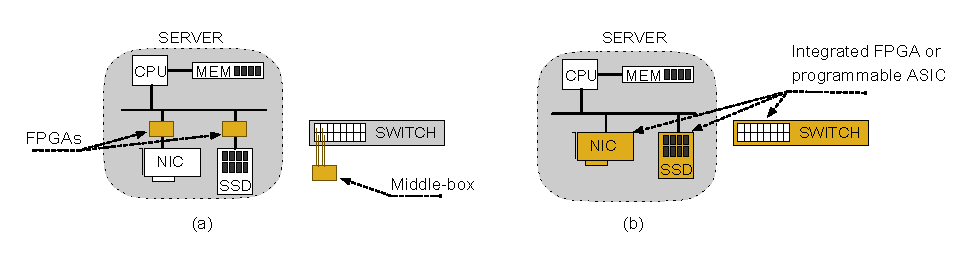
\includegraphics[bb=0 0 451 108]{fig_bump_internal.eps} %% 0.75
    \caption{Alternative in-network computing and near-storage processing
      platforms.
      (a) Using ``bump-in-the-wire'' FPGAs or network ``middle-boxes'' to create
      early application logic sites.
      (b) Leveraging programmability within the device for application logic.}
    \label{fig:bump_internal}
\end{figure}


The networking and storage stacks have always carried some computing power.
Network switches can triage billions of packets per second.
Solid-state drives (SSDs) can scramble and encode gigabytes of data per second
(for error correction purposes~\cite{cai17}).
Despite such computing power, applications have no access to how the
devices process the data, other than by issuing IO requests.
The functionality of these devices has been closed to changes.  Opening them
would require supporting a certain level of \emph{programmability}.


Nonetheless, the benefits of executing application logic close to networking and
storage devices are known~\cite{fang19, teubner13}.
New algorithms that take advantage of proximity to the data become viable and
provide both performance and power consumption gains.
Figure~\ref{fig:bump_internal}(a) illustrates how FPGAs and network
``middle-boxes'' can create these opportunities.


The lack of programmability in network and storage devices has impacted not
only applications.
It has also hindered the advancement of these platforms.
On the networking side, new protocols emerge that depend heavily on hardware to
run at high-speeds.
\emph{Fixed-function} devices, the ones that have their functionality ``baked''
into the hardware, may need to undergo a full, lengthy development cycle before
they can run new protocols.
Recently, a solution emerged where a new class of networking devices started
supporting programmability (e.g., in programmable switches~\cite{bosshart13} and
``smart'' NICs~\cite{zilberman14}).
The protocols these devices run are expressed as software programs.


The need for programmability also emerged on storage platforms recently.
SSDs are designed to shield applications from the intricacies of managing
flash memory.
However, evidence appeared that SSDs often miss the right performance decisions
because of the separation between it and the
applications~\cite{bjorling17}.
A more \emph{modular} SSD design, deemed \emph{open-channel}, was proposed that
allows a host (a server), rather than the SSD itself, to make certain low-level
decisions.
The modules that run on the host are software-based, therefore programmable.


Developers soon realized that the programmability could also be used by
applications.
It made it possible to inject application code directly into the networking and
storage stacks.
Figure~\ref{fig:bump_internal}(b) depicts such a scenario.
\emph{In-network computing} and \emph{near-storage processing} emerged as the
disciplines that leverage processing power in the network and storage stacks,
respectively, for application purposes.


An application that benefits from INC or NSP contains, by definition, algorithms
running in different computing elements of a system.
These algorithms ought to communicate at high speed.
The most commonly used interconnect for such systems has been based on the
PCIe bus standard~\cite{budruk03}.
At this time, the standard is being revised to operate at higher speeds.
PCIe is also being extended with mechanisms to support cache coherence protocols
to run atop of it~\cite{ccix19, cxl19}.


Despite their potential, INC and NSP platforms are not without challenges.
INC is a more mature technology with increasingly popular programmable models
that shield the developer from the intricacies of the devices.
Such programming models, however, are quite different from a general-purpose
CPU’s.
In contrast, NSP often uses general-purpose processors---but much less powerful
ones than server-class CPUs.
In both cases, porting algorithms to these platforms requires rethinking the
algorithms to fit either a different model or a less-powerful environment.


In this paper, we elaborate on the above challenges and opportunities of
adopting INC and NSP as platforms to improve application performance.
We summarize the contributions of this paper are as follows:
\begin{itemize}
  \setlength{\itemsep}{0pt}
  \setlength{\parsep}{0pt}
  \setlength{\parskip}{0pt}
  \setlength{\topsep}{0pt}
  \setlength{\partopsep}{0pt}
\item We discuss the evolution and recent advancements of INC and NSP platforms;
\item We present specific computation tasks that can benefit from them;
\item We describe the challenges that still remain in order to use INC and NSP
  as application platforms;
\item Finally, we present the benefits of adopting the current generation of INC
  and NSP.
\end{itemize}


The rest of this paper is structured as follows.
We discuss the programmability of the network and storage stacks in more detail
in Section~\ref{sec:background}.
We show examples of computing paths that can leverage INC and NSP capabilities in
Section~\ref{sec:data_paths}.
We comment on the evolution of the PCIe interconnect and the possibilities it
opens in Section~\ref{sec:interconnects}.
We discuss the challenges and opportunities of adopting INC and NSP platforms in
Section~\ref{sec:challenges}.
We elaborate on how ready for adoption the technologies are in
Section~\ref{sec:discussion}, before concluding in Section~\ref{sec:conclusion}.


\section{An Abridged History of INC and NSP}
\label{sec:background}

There have been many attempts to conciliate speed and flexibility in
networking hardware devices.
Figure~\ref{fig:evolution_net} depicts the main ideas behind the relevant
milestones in that context.


\begin{figure}[h]
  \centering
  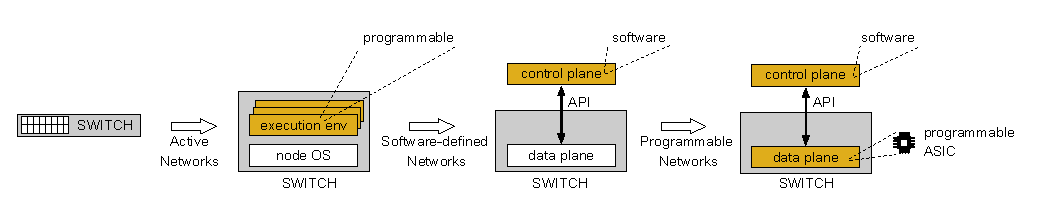
\includegraphics[bb=0 0 483 88]{fig_evolution_net.eps} %% 0.68
  \caption{Evolution of the network stack towards programmability.}
  \label{fig:evolution_net}
\end{figure}


\emph{Active Networks}, one of the first attempts, proposed a standard
architecture for more flexible network devices~\cite{calvert98}.
The goal of the architecture is to enable changes to the device
behavior—--typically to implement new protocols—--via the execution of
user-driven customization.
There are two main components in such a device.
First, a node operating system that manages basic IO functionality, including
processing, storage, and transmission.
Second, multiple Execution Environments (EE) that support the execution of
programs containing packet-processing logic.
Applications can inject code into the device through an API, which generates
special packets for the device to execute.
Active networks proved to be very flexible; however, they ran considerably
slower than their fixed-function counterparts.


\emph{Software-Defined Networks} (SDN), a later attempt at a more flexible
network, is also centered around a standard device
architecture~\cite{kreutz15}.
The main feature of the architecture is the separation of the control plane
(policy definition) from the data plane (policy implementation).
The control plane would contain information such as routing tables; the data
plane would use that information to forward packets without sacrificing speed.
An SDN device could adopt a new protocol if the SDN standard recognizes that
protocol.
Introducing new protocols, however, still required changes in the SDN standard
itself and sometimes also on the devices.
The main issue was that SDN only supports custom logic on the control plane.
Protocols that depended on special per-packet logic need to send these packets
to the control plane, which in turn processes them, pushing the results back to
the data plane.
The additional path cannot sustain \emph{line-rate}, as one calls the individual
port speed of a switch.


In a more recent development, \emph{Programmable Dataplanes} (also referred to
as \emph{Programmable Networks}) allowed custom logic on the data
plane~\cite{bifulco18}.
The cornerstone of this technology is a generation of programmable ASICs (chips)
that supports a certain degree of stateful packet processing without compromising
speed~\cite{bosshart13}.
This balance is captured by a programming model called Protocol Independent
Switch Architecture (PISA)~\cite{sivaraman16}.
PISA shields the programmer from various device intricacies and, because it was
designed to be protocol-independent, it proved adept at expressing application
computations as well.
Programmable networks created the conditions for a new generation of
applications to push specialized logic into the network, i.e., to perform
\emph{in-network computing}.


\vspace{1em}
We now turn our attention to the evolution of the storage stack.
Just as with networks, the idea of near-storage processing is not new, but the
driver for altering this stack has been more application-centric than in
networking.
In the early 2000s, a seminal proposal, called \emph{Active Disks}, gained
traction that aimed at transforming hard drive controllers into data-processing
platforms~\cite{riedel01}.
These controllers often carried a small, general-purpose processor that was
somewhat over-dimensioned for its purpose.
Applications could place logic on that processor, and access/modify the data
blocks that were streaming in and out of the hard drive.
The computing power of these controllers ultimately proved to be underwhelming,
and the industry saw little need to improve them.


Eventually, SSDs based on NAND-flash displaced hard drives in many applications.
Managing flash memory requires considerably more computing power than a magnetic
medium, and flash memory error rates are very high, which requires
computational-intensive error correction techniques~\cite{cai17}.
Moreover, the industry decided that SSDs should be drop-in replacements for hard
drives.
SSDs execute internally a compatibility layer called Flash Translation Layer
(FTL) for that purpose~\cite{chung09}.
All these factors turn SSDs into relatively powerful embedded devices.


A proposal soon emerged to leverage SSD controllers for database query
processing using \emph{smart SSDs}~\cite{do13}.
As with active disks, the computing capacity on early devices was not sufficient
for most computations in practice~\cite{do19}.
It would take a new generation of devices to accommodate fast database
logic~\cite{kim16}.
However, the industry focus was more on making devices faster than on making
them smarter.
Performance wasting was an issue, as the FTL not always makes the best decisions
from an application's point of view.
Some efforts emerged that tried to make SSD architectures more open to
configurations.
Figure~\ref{fig:evolution_ssd} captures the essential steps of this effort.


\begin{figure}[h]
  \centering
  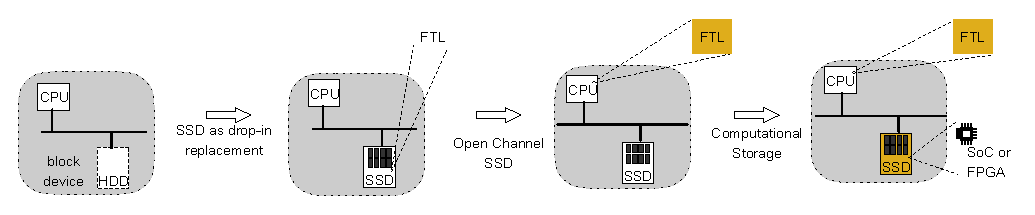
\includegraphics[bb=0 0 481 87]{fig_evolution_ssd.eps} %% 0.68
  \caption{Evolution of the storage stack towards programmability.}
  \label{fig:evolution_ssd}
\end{figure}

\emph{Open Channel SSDs} appeared from a growing understanding that many of the
FTL tasks were better performed leveraging application
knowledge~\cite{bjorling17}.
In an open-channel SSD, some of the FTL responsibilities are removed from the
device.
Instead, they run on the host housing the SSD or even inside individual
applications~\cite{ouyang14}.
Naturally, these devices expose a lower-layer view of the underlying flash
medium.


With more exposure to SSD architectural details, several works emerged to build
tooling around these devices.
These efforts range from frameworks to program SSD controllers~\cite{picoli20},
to performance measurement tooling~\cite{lerner20}, to even full SSD rapid
prototyping platforms~\cite{kwak20}.
At the same time, a class of works appeared that deploy application code on
SSDs, making them a \emph{Computational Storage} platform~\cite{picoli19, ruan19,
woods14}.
The common thread in these works is that they increase the existing computing
power of the devices by building them on platforms such as a System-on-a-Chip
(SoC) or an FPGA.
The tooling and the additional computing capacity paved the way for
\emph{Near-Storage Processing}.


One problem that remains open, however, is the lack of a consensus around a
programming model.
While there are recent proposals in that sense (e.g., in~\cite{gu16}), these
models leave many aspects undefined.
For instance, they have not addressed how to interface application logic with
internal device mechanisms.
An application that wishes to influence the IO scheduling policy of a device
directly has no means to do so.
There is also no consensus on how to shield an application developer from
specific aspects of different devices.


\section{Alternative Computing Paths}
\label{sec:data_paths}

INC and NSP  provide alternative sites beyond a CPU where applications can place
logic.
This fundamentally changes the traditional data movement patterns we see in
CPU-centric algorithms, potentially bringing performance and power savings
benefits.
We illustrate these possibilities in this section by presenting and discussing
several use cases in large-scale data management.


\subsection{In-Network Data Aggregation}
\label{ssec:aggr}

Data aggregation is a very common operation in data management.
Aggregation involves grouping data by specific criteria and calculating
summaries over each group.
A typical example is the \texttt{GROUP BY} clause in \texttt{SQL}.
When the data volume is large, the operation can involve several servers,
e.g., as in a rack-wide computation.
Figure~\ref{fig:flow_1}(a) illustrates one possible way to solve such a distributed
aggregation.


The servers agree on how to partition the data, taking into consideration the
grouping key.
This divides the work into disjoint, independent tasks.
Each server reshuffles its data while performing the aggregation over its
assigned partition, as data arrives.
Eventually, all the machines send their aggregation results to an elected
server, which combines them into a global result.
Note that throughout all these interactions, the switch performs data
transmissions only.


\begin{figure}[h]
    \centering
    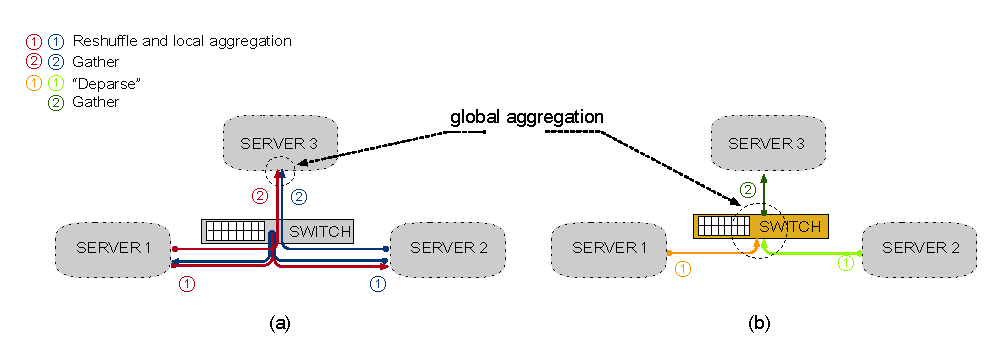
\includegraphics[bb=0 0 462 156]{fig_flow_1.eps} %% 0.75
    \caption{Data aggregation scenario (e.g., SQL GROUP BY).
      (a) With a ``passive'' switch, the servers first repartition the data
      and work on aggregating its assigned partition locally.
      Then, an elected server gathers all partitions and performs the global
      aggregation.
      (b) On an INC platform, an ``active'' switch can, in typical situations,
      perform the global aggregation in one step and transmit the results to an
      elected server.
      We use a given color to represent each unique data stream in the
      computation.
      }
    \label{fig:flow_1}
\end{figure}


In Figure~\ref{fig:flow_1}(b), we show that using the switch as an active
element simplifies the entire computing path~\cite{lerner19}.
We assume that the switch is programmable and that it can be leveraged to hold
an entire aggregation table.
The size of such a table is often manageable, as it is proportional to the
number of groups involved, rather than the size of the dataset.
Note that the servers need not reshuffle the data nor perform an aggregation on
a partition.
Because programmable switches perform computations at line-speed, the
aggregation table on the switch will be completed as soon as the last server
finishes transmitting its tuples, and can then be sent immediately to an elected
server.


Not all computations are suitable for INC deployment.
The important caveats include: (a) the number of steps the switch can execute
over each packet is limited; (b) the kind of instructions the switch can perform
is also constrained; and (c) programmable network devices adhere to a
programming model that imposes a \emph{forward logic}-style onto algorithm
design.
Loops and complex branching are strongly discouraged, although possible.
In practice, these restrictions reduce the choices of data structures the switch
can support.
In particular, the aggregation described in Figure~\ref{fig:flow_1}(b) requires
a hash table to be adapted to INC constraints.
In this case, the number of collisions can be handled on the switch up to a
certain bound.
Relaxing this constraint involves using a technique called
``overflowing''~\cite{lerner19}, which allows treating long collision chains
outside the switch without a noticeable performance penalty in most cases.

These limitations notwithstanding, a large class of computations can benefit from
INC platforms~\cite{ports19}.
Moreover, processing data on the switch tends to scale well as the number of
servers grows in the cluster.
The number of switches naturally grows with the number of servers.


\subsection{Near-Storage Checkpoint Derivation}
\label{ssec:cp_derivation}

We now describe an opportunity that arises specifically in an in-memory database
system.
Like most DBMSs, in-memory databases guarantee durability using a persistent
transaction log.
Because the log can get arbitrarily long, it would be impractical to recover
from a crash just by replaying it.
Therefore, databases also perform a periodical checkpoint (e.g., by taking a
snapshot) of the current memory state and write it to persistent storage, often
SSDs.
A recovery algorithm can load the snapshot and replay the portion of the log
acquired after the checkpoint.
In in-memory databases, the log and checkpoint are the only workloads written to
disk.


The logging and checkpointing processes compete for both disk and memory
bandwidth.
Figure~\ref{fig:flow_2}(a) shows these contention points.
The checkpointing process reads the database contents from the main-memory while
it is being queried/modified.
The checkpointing process also issues write requests to the SSD, which have to
be scheduled along with the logging workload.
The contention is responsible for the throughput reduction that many systems
experience during checkpoints.


\begin{figure}[h]
  \centering
  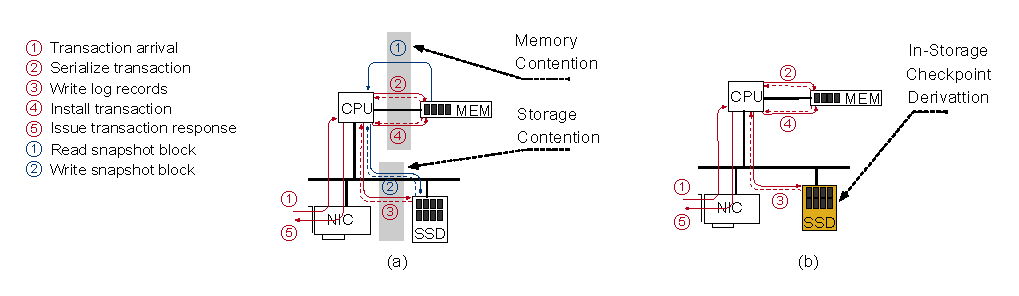
\includegraphics[bb=0 0 473 126]{fig_flow_2.eps} %% 0.75
  \caption{Checkpoint computation scenario.
    (a) Transaction logging (red) and checkpoint (blue) are two parallel
    processes.
    They compete for memory and disk bandwidth.
    (b) A checkpoint could be derived by processing the transaction log inside
    an SSD.
    The solid lines represent data; the dashed ones, control and/or return.
  }
  \label{fig:flow_2}
\end{figure}


The key observation here is that partial snapshots, which can serve as
checkpoints, can be derived from the log stream directly.
We believe that such derivations may very well occur inside a smart SSD.
We show in Figure~\ref{fig:flow_2}(b) that once we move that process to the
device, the contention points disappear.


Note, however, that the processing power on an SSD is far smaller than that of a
general-purpose CPU.
We cannot possibly expect to move the same algorithm we used on a CPU into an
NSP platform and obtain similar performance results.
Creating a checkpoint derivation algorithm for an SSD requires finding snapshot
approximations that the device can process at the necessary pace.
We comment on Section~\ref{sec:challenges} how specific architectural changes on
smart SSDs can make this task easier.


\subsection{Low Latency Database Replication}
\label{ssec:low_latency}


Another code path that can benefit from either INC or NSP is that of a replica
node in a database system.
On a master node, transactions need to be serialized via a concurrency control
algorithm.
The latter typically runs on a CPU.
The replica node code-path is simpler because the serial order of the
transactions was already determined.
The CPU takes the modifications coming from the network card and persists them
on disk in the same order it received them.
Subsequently, it updates its data structures and sends a notification to the
master node that it accepted the transaction.
Figure~\ref{fig:flow_3}(a) depicts such an interaction.


\begin{figure}[h]
  \centering
  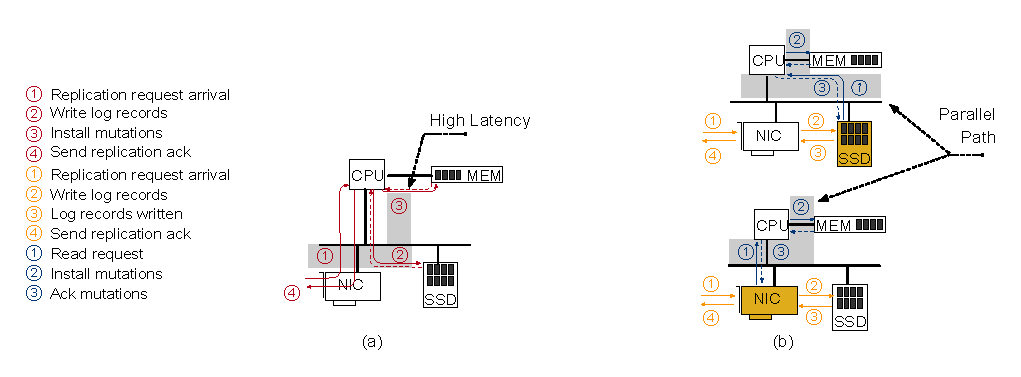
\includegraphics[bb=0 0 474 165]{fig_flow_3.eps} %% 0.75
  \caption{Database replica node scenario.
    (a) Each transaction log entry is first persisted in storage and then
    applied to memory, as the CPU coordinates the replication.
    (b) If an ``active'' NIC or SSD coordinates the process, the persistence and
    memory update paths can proceed in parallel.
  }
  \label{fig:flow_3}
\end{figure}


Note that the replica code path incurs in latency.
The master node may be withholding the original transaction until the
replication path is completed.
We can optimize this code path in at least two ways.
Using NSP, the NIC would send the modification stream directly to a smart SSD.
In turn, the SSD could be programmed to coordinate the interaction instead of
the CPU.
The SSD would notify the NIC after it persisted the changes, reducing the
latency.
It would also, in parallel, allow the CPU to read (and perform) the
modifications.
An alternative path exists where the NIC itself would perform the coordination.
Figure~\ref{fig:flow_3}(b) shows both cases.
This scenario involves having the NIC and the SSD communicate without any CPU
intervention.
This type of communication is called peer-to-peer DMA~\cite{budruk03} and it has
been used in other contexts before, such as direct access to a remote disk
(e.g., NVMe-over-Fabrics~\cite{guz18}).


\section{Upcoming Interconnects}
\label{sec:interconnects}

INC and NSP platforms rely on an interconnect to communicate with other
computing elements in a system.
PCIe has been the \emph{de facto} interconnect for quite a
while~\cite{budruk03}.
PCIe is a point-to-point bus with a variable number of lanes dedicated to
devices.
Each lane can transfer close to 1GB/s on the current standard version, Gen 3.
Cards attached to the bus can use 1$\times$, 2$\times$, 4$\times$, 8$\times$, or
16$\times$ lanes to achieve a theoretical maximum of 16 GB/s bidirectional
bandwidth.


Newer devices are creating the need for faster speeds.
For instance, the standard NIC port speeds are about to go from 100 Gb/s to 400
Gb/s, which a single Gen 3 PCIe slot can no longer support.
The PCIe standard had moved to 2 GB/s lanes on Gen 4.
The following iteration of the standard, Gen 5, brings 4 GB/s lanes with a
theoretical bi-directional bandwidth of 64GB/s for 16$\times$ device.


There is another compelling feature that new versions of PCIe buses will bring:
cache coherence.
This feature allows computing elements to negotiate who may be caching a given
portion of memory at any given time.
It also determines who has the license to write to that memory address.
Coordinating access to single memory address allows all the computing elements
to share a single view of memory, as Figure~\ref{fig:coherence}(a) shows.
There are two flavors of coherency: one in which the CPU has a prominent role in
controlling the memory, called \emph{asymmetric}, and one in which all computing
elements play a similar role, called \emph{symmetric}.


\begin{figure}[h]
  \centering
  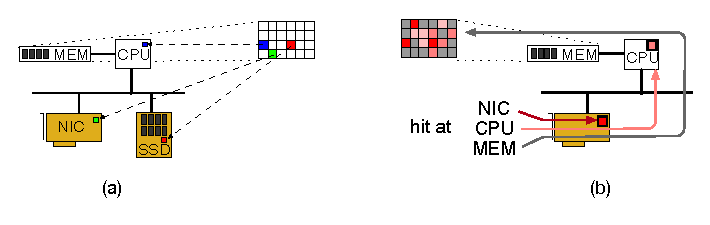
\includegraphics[bb=0 0 325 92]{fig_coherence.eps} %% 0.75
  \caption{Cache coherency scenarios: (a) a NIC and an SSD may be responsible
    for writing to specific addresses in memory that can be read by other
    elements, and (b) a NIC can be responsible for caching (and writing to) very
    hot pages while leaving the CPU responsible for less accessed pages.
  }
  \label{fig:coherence}
\end{figure}


At the time of writing, there are four upcoming interconnects offering both high speed and coherence:
CAPI~\cite{stuecheli15}, CCIX~\cite{ccix19}, CXL~\cite{cxl19} and
Gen-Z~\cite{knebel19}.
CCIX and Gen-Z support symmetric coherence, unlike CAPI or CXL, which support
asymmetric coherence.
CAPI is a competing standard to PCIe.
CCIX and CXL use only PCIe, while Gen-Z can use ethernet as well as PCIe.
The range of PCIe is short enough to work only within the confines of a chassis,
while ethernet allow to connect across chassis.
This opens up the possibility of CCIX or CXL being applied simultaneously with
Gen-Z to form coherence domains that cross server boundaries.


Cache coherency allows for new INC and NSP design use cases.
For instance, one may extend the caching hierarchy beyond the CPU.
Figure~\ref{fig:coherence}(b) illustrates this possibility.
Some distributed applications may cache hot data items in the
NIC~\cite{tokusashi18}.
With coherence, the NIC can also request write access to such an item and update
it.
Any other computing element that requests to cache that address would then see
the updates.


\section{Challenges and Opportunities}
\label{sec:challenges}

We mentioned above some immediate difficulties that arise when deploying current
generation INC and NSP platforms.
In this section, we elaborate on further challenges and opportunities that we
believe would unlock more of the potential of these platforms.


\softsubsec{In-Network Stateful Computations.}
%
Data management primarily involves stateful computations, i.e., algorithms that
access a result from a previous iteration and generate a new result at the
next one.
The aggregation operation discussed in Section~\ref{ssec:aggr} is one such
algorithm.
Maintaining state in-network, particularly in switches, is currently very
challenging.
Programmable switches rely on high-speed memories that, for cost reasons, are
present in limited amounts.
Moreover, switches have a very strict ``allowance'' of how many instructions
they can execute per packet and what those instructions can do.
These restrictions make maintaining data structures other than a hash
table on a switch possible but difficult.
Even some common operations on hash tables, such as collision management,
require some adapting, as we discussed above.


We miss a computing model that can relax those restrictions to a certain extent
while still keeping the ability to run logic at line-speed.
Supporting such a model would most likely require introducing new hardware onto
programmable switches.
We believe such a model is possible, but the field of in-network computing is
still new.
There is not yet a clear list of missing operations from applications beyond
networking protocols on which to base new switch hardware capabilities.


\softsubsec{SSD-Application Interface.}
%
A regular SSD makes several decisions such as IO scheduling and page mapping
based solely on observing the stream of IO commands it receives~\cite{nam11}.
When application logic executes inside the device, it becomes an additional
stream of IO commands.
The internal and external streams would likely compete with one another.
A straightforward way to manage the new internal streams is to pretend they came
from outside and to proceed as usual.


An alternative way would be to allow the application logic and the device to
interact.
Consider again the checkpoint derivation scenario we describe in
Section~\ref{ssec:cp_derivation}.
It generates new IO requests at a given pace.
Depending on the current load on the SSD, the checkpoint stream can be too fast or
too slow for the device to handle.
Ideally, we want a means for the device and the application logic to negotiate
that pace.
There is an opportunity here to establish a communication model that supports
this kind of interaction.


\softsubsec{SSD Channel Architecture.}
%
An SSD's bandwidth and capacity are a result of combining many relatively
limited NAND flash \emph{packages} (chips)~\cite{micheloni12}.
A typical arrangement is to group the packages in disjoint sets called
\emph{channels}.
There are anywhere between 8 to 32 channels in a typical SSD.
This arrangement has proved adequate when data pages are transferred in and out
of the device.


The introduction of application logic into an SSD, however, can cause data
pages to be moved \emph{across packages}---possibly between channels.
For instance, we describe in Section~\ref{ssec:cp_derivation} how an NSP process
can read pages from a transaction log and write them, after some manipulation,
as pages of a checkpoint.
In a traditional SSD architecture, this pattern would consume bandwidth from
both the origin and the destination channels.
We believe that there may be other package interconnect architectures
beyond channels that are more suited to the data movements above.
To the best of our knowledge, there has been no study about interconnects that
involve architectures other than fixed channels.


\softsubsec{Code-Variant Generation and Selection.}
%
INC and NSP platforms introduce additional hardware heterogeneity to computing
platforms.
An algorithm implementation that works well on a given switch may not work on a
different one, due to architectural differences.
The generation and selection of variant implementations is a known problem; it
appeared before in domains such as GPUs~\cite{rosenfeld15}.


To complicate matters, some algorithms are flexible enough to be deployed either
on a NIC or on the switch to which it connects.
The selection of the most appropriate platform constitutes an optimization step
that compounds to the variant selection problem above.
Currently, the programmer is responsible for making such choices.
There is an opportunity for creating higher-level tooling that would aid in
these decisions.


\softsubsec{Runtime Resource Management.}
%
In a regular setting, the operating system mediates every single network and
storage IO between applications and devices.
The OS does so by interposing itself between the two.
What, then, should be the role of the OS when a portion of the applications
reside \emph{inside} the device?


One potential solution is to accept that applications may want to access a device
directly, without mediation.
Such is the premise of Arrakis~\cite{peter15}, which tricks an application into
interacting with virtual versions of the devices, and redesigns the kernel to
provide the expected protections under such assumptions.


\section{Discussion}
\label{sec:discussion}

Notwithstanding the challenges and opportunities described in the previous
section, INC and NSP platforms are a reality.
The question arises as to whether they are ready for adoption.
In this section, we break this question into a list of sub-questions and answer
each one in turn.


\softsubsec{Are there diverse offerings of INC and NSP platforms?}
%
INC can be realized by many different hardware targets, both on switches and
NICs.
In terms of programmable switches, there are at least three silicon
manufacturers producing programmable ASICs: Barefoot (Intel)
Tofino~\cite{barefoot}, Broadcom Trident 4~\cite{broadcomT4}, and Cavium
(Marvel) Xpliant~\cite{cavium}.
Together, these chips appear in several commercial offerings from companies such as
Cisco and Arista.
SmartNICs are also widely available, ranging from FPGA-centric accelerators such as
Xilinx Alveo~\cite{xilinx} to more software-oriented platforms such as
Netronome~\cite{netronome}.
The offering for programming languages and abstractions is also diverse.
A prevalent language is \texttt{P4}~\cite{bosshart14}, but there are variations
such as \texttt{NPL}~\cite{broadcomnpl} and even \texttt{C} libraries in some
cases~\cite{netronome}.


NSP is also a rich environment with many prototyping and commercial platforms
available.
For instance, SSDs are starting to emerge that introduce application
specializations.
Samsung has recently announced the KV-SSD, which incorporates Key Value store
logic within its firmware~\cite{ki17}.
One issue with such offerings is that they add application functionality
but do not expose programmability.
The interested reader should look at~\cite{picoli20} for an extensive list of
specialized SSD and NSP-platforms available at the time of writing.


\softsubsec{What are the advantages of INC and NSP compared to ``CPU-centric''
alternatives?}
%
While there is no study yet of an exacale platform that resorts to both INC and
NSP, the expected benefits are a combination of increased performance, lower
energy expenditure, and lower CPU utilization.
There a numerous works that provide partial results.

For INC, data manipulations such as the one described in Section~\ref{ssec:aggr}
were studied before~\cite{lerner19}.
We can expect to see the performance of many typical queries improve by a factor of
2$\times$\ by using programmable switches at moderate network
speeds.
The power consumption in these switches is estimated to be only 12.4\% higher
than their fixed-function counterparts, and, anecdotally, the switches cost
about the same.
The operations-per-Watt ratio on some INC platforms such as smartNICs was
also studied before~\cite{tokusashi18}.
For instance, a variant of the caching scenario we discussed in
Section~\ref{sec:interconnects} reports a 17$\times$ better power utilization as
compared to a regular CPU.


NSP platforms deliver similar benefits.
According to~\cite{kim16}, the performance of scans and joins can see
performance improvements between 5$\times$ and 47$\times$, the cost of equipping
an SSD to support near-storage processing is less than 1\% of its total cost,
and the energy-efficiency compared to performing those operations on a CPU can be up
to 45$\times$ better.


\softsubsec{Are there standards in place to guarantee the portability and
longevity of the solutions?}
%
There is a big difference from a standardization point of view between INC and
NSP technologies.
As mentioned above, INC has broadly embraced \texttt{P4} as a programming language.
The latest edition of the language, \texttt{P4$_{16}$}, allows different target
platforms to express their capabilities.
A compiler can generate specific code from a unique source to different, maybe
even disparate, devices.
These feature makes the language flexible enough to work on future devices,
which can only help its adoption.


In contrast, there is not yet a consensus on how computational storage should be
programmed.
We even miss a standard around what an open-channel SSD should be, which would
arguably be a necessary step.


\section{Conclusion}
\label{sec:conclusion}

In this paper, we reviewed how the evolution of the network and storage stacks
have unlocked their computing power.
Applications can not only request services from these stacks, but also
embed logic into them.
We showed that with a careful redesign, algorithms running on INC or NSP
platforms could present a reduced amount of data movement, lower CPU
utilization, less energy consumption, or a combination of these.


We also discussed several challenges that INC and NSP still face.
Despite these limitations, we commented on a current generation of INC- and
NSP-enabled devices that are available off-the-shelf.
We believe that the emergence of the network and storage stacks as computing
elements creates promising ways to scale typical data management computations.


\softsec{Acknowledgments.}
%
This project has received funding from the European Research Council (ERC) under
the European Unions Horizon 2020 research and innovation programme (grant
agreement 683253/GraphInt).


\begin{thebibliography}{10}
\itemsep=1pt
\begin{small}

\bibitem{barefoot}
  \newblock Barefoot Tofino and Tofino 2 Switches.
  \newblock https://www.barefootnetworks.com/products/brief-tofino-2/.

\bibitem{bifulco18} R.~Bifulco, and G.~R\'etv\'ari.
  \newblock A Survey on the Programmable Data Plane: Abstractions, Architectures, and Open Problems.
  \newblock {\em HPSR}, June, 2018.

\bibitem{bjorling17} M.~Bj{\o}ling, J.~Gonz\'alez, and P.~Bonnet.
  \newblock Lightnvm: The Linux Open-Channel SSD Subsystem
  \newblock {\em FAST}, February, 2017.

\bibitem{broadcomnpl} Broadcom NPL.
  \newblock Network Programming Language.
  \newblock {\em https://nplang.org/}.

\bibitem{broadcomT4} Broadcom.
  \newblock Broadcom Trident 4.
  \newblock {\em https://www.broadcom.com/products/ethernet-connectivity/switching/strataxgs/bcm56880-series}.

\bibitem{bosshart13} P.~Bosshart, G.~Gibb, H.-S.~Kim, G.~Varghese, N.~McKeown, M.~Izzard, F.~Mujica, and M.~Horowitz.
  \newblock Forwarding Metamorphosis: Fast Programmable Match-Action Processing in Hardware for SDN.
  \newblock {\em SIGCOMM CCR}, 43(4):99--110, 2013.

\bibitem{bosshart14} P.~Bosshart., D.~Daly, G.~Gibb, M.~Izzard, N.~McKeown, J.~Rexford, C.~Schlesinger, D.~Talayco, A.~Vahdat, G.~Varghese, and D.~Walker.
  \newblock P4: Programming protocol-independent packet processors.
  \newblock {\em ACM SIGCOMM CCR}, 44(3):87--95, 2014.

\bibitem{budruk03} R.~Budruk, D.~Anderson, and E.~Solari.
  \newblock PCI Express System Architecture.
  \newblock {\em Pearson Education}, 2003.

\bibitem{cai17} Y.~Cai, S.~Ghhose, E.F.~Haratsch, Y.~Luo, and O.~Mutlu.
  \newblock Error Characterization, Mitigation, and Recovery in Flash-Memory-Based Solid-State Drives.
  \newblock {\em Proc. of the IEEE}, 105(9), 1666--1704, 2017.

\bibitem{calvert98} K.L.~Calvert, S.~Bhattacharjee, E.~Zegura, and J.~Sterbenz.
  \newblock Directions in Active Networks.
  \newblock {\em IEEE Comm. Magazine}, 36(10):72--78, 1998.

\bibitem{cavium} Cavium.
  \newblock XPliant Ethernet Switch Product Family.
  \newblock {\em www.cavium.com/XPliant-Ethernet-Switch-Product-Family.html}

\bibitem{ccix19} CCIX Consortium.
  \newblock An Introduction to CCIX.
  \newblock {\em White Paper}, https://www.ccixconsortium.com/wp-content/uploads/2019/11/CCIX-White-Paper-Rev111219.pdf

\bibitem{chung09} T.-S.~Chung, D.-J.~Park, S.~Park, D.-H.~Lee, S.-W.~Lee, and H.-J.~Song.
  \newblock A Survey of Flash Translation Layer.
  \newblock {\em J. of Syst. Archit.}, 55(5--6):332--343, 2009.

\bibitem{cxl19} D.D.~Sharma.
  \newblock An Introduction to Compute Express Link.
  \newblock {\em White Paper}, https://docs.wixstatic.com/ugd/0c1418\_d9878707bbb7427786b70c3c91d5fbd1.pdf.

\bibitem{do13} J.~Do, Y.S.~Kee, J.M.~Pzatel, C.~Park, K.~Park, and D.J.~DeWitt.
  \newblock Query Processing on Smart SSDs: Opportunities and Challenges.
  \newblock {\em SIGMOD}, June, 2013.

\bibitem{do19} J.~Do, S.~Sengupta, and S.~Swanson.
  \newblock Programmable Solid-State Storage in Future Could Datacenters.
  \newblock {\em CACM}, 62(6):54--62, 2019.

\bibitem{fang19} J.~Fang, Y.T.B.~Mulder, J.~Hidders, J.~Lee, and H.P.~Hofstee.
  \newblock In-Memory Database Acceleration on FPGAs: A Survey.
  \newblock {\em VLDB Journal}, October, 2019.

\bibitem{gu16} B.~Gu, A.S.~Yoon, D.H.~Bae, I.~Jo, J.~Lee, and J.~Yoon.
  \newblock Biscuit: A Framework for Near-Data Processing of Big Data Workloads.
  \newblock {\em SIGARCH Comp. Arch. News}, 44(3):153--165.

\bibitem{guz18} Z.~Guz, H.~Li, A.~Shayesteh, and V.~Balakrishnan.
  \newblock Performance Characterization of NVMe-over-Fabrics Storage Disaggregation.
  \newblock {\em ACM Trans. on Storage}, 14(4):1553--3077, 2018.

\bibitem{ki17} Y.-S.~Ki.
  \newblock Key Value SSD Explained – Concept, Device, System, and Standard.
  \newblock {\em SNIA SDC}, September, 2017.

\bibitem{kim16} S.~Kim, H.~Oh, C.~Park, S.~Cho, S.-W.~Lee, and B.~Moon.
  \newblock In-Storage Processing of Database Scans and Joins.
  \newblock {\em Inf. Sci.}, 327(C):183--200, 2016.

\bibitem{knebel19} P.~Knebel, D.~Berkram, A.~Davis, D.~Emmot, P.~Faraboschi, and G.~Gostin.
  \newblock Gen-Z Chipset for Exascale Fabrics.
  \newblock {\em HotChips}, August, 2019.

\bibitem{kreutz15} D.~Kreutz, F.M.V.~Ramos, P.E.~Ver\'issimo, C.E.~Rothenberg, S.~Azodolmolky, and S.~Uhlig.
  \newblock Software-Defined Networking: A Comprehensive Survey.
  \newblock {\em Proc. of the IEEE}, 103(1):14--76, 2015.

\bibitem{kwak20} J.~Kwak, S.~Lee, K.~Park, J.~Jeong, and Y.H.~Song.
  \newblock Cosmos+ OpenSSD: Rapid Prototype for Flash Storage Systems.
  \newblock {\em ACM Trans. on Storage}, to appear.

\bibitem{lerner19} A.~Lerner, R.~Russein, and P.~Cudr\'e-Mauroux.
  \newblock The Case for Network Accelerated Query Processing.
  \newblock {\em CIDR}, January, 2019.

\bibitem{lerner20} A.~Lerner, J.~Kwak, S.~Lee, K.~Park, Y.H.~Song, and P.~Cudr\'e-Mauroux.
  \newblock It Takes Two: Instrumenting the Interaction between In-Memory Databases and Solid-State Drives.
  \newblock {\em CIDR}, January, 2020.

\bibitem{micheloni12} R.~Micheloni, A.~Marelli, and S.~Eshghi.
  \newblock Inside Solid State Drives (SSDs).
  \newblock {\em Springer}, 2012.

\bibitem{nam11} E.H.~Nam, B. S. J.~Kim, H.~Eom, and S. L.~Min.
  \newblock Ozone (O3): An Out-of-Order Flash Memory Controller Architecture.
  \newblock {\em IEEE Transactions on Computers}, 60(5):653--666, 2011.

\bibitem{netronome} Netronome.
  \newblock Agilio CX SmartNICs.
  \newblock {\em https://www.netronome.com/products/agilio-cx/}

\bibitem{ouyang14} J.~Ouyang, S.~Lin, S.~Jiang, Z.~Hou, Y.~Wang, and Y.~Wang.
  \newblock SDF: Software-Defined Flash for Web-Scale Internet Storage Systems.
  \newblock {\em ASPLOS}, 2014.

\bibitem{peter15} S.~Peter, J.~Li, I.~Zhang, D.R.K.~Ports, D.~Woos, A.~Krishnamurthy, T.~Anderson, and T.~Roscoe.
  \newblock Arrakis: The Operating System Is the Control Plane.
  \newblock {\em ACM TOCS}, 33(4), 2015.

\bibitem{picoli19} I.L.~Picoli, P.~Bonnet, and P.~T\"oz\"un.
  \newblock LSM Management on Computational Storage.
  \newblock {\em DaMoN}, July, 2019.

\bibitem{picoli20} I.L.~Picoli, N.~Hedam, P.~Bonnet, and P.~T\"oz\"un.
  \newblock Open-Channel SSD (What Is It Good For).
  \newblock {\em CIDR}, January, 2020

\bibitem{ports19} D.R.K.~Ports, and J.~Nelson.
  \newblock When Should The Network Be The Computer.
  \newblock {\em HotOS}, May, 2019.

\bibitem{riedel01} E.~Riedel, C.~Faloutsos, G.A.~Gibson, and D.~Nagle.
  \newblock Active Disks for Large-Scale Data Processing.
  \newblock {\em IEEE Computer}, 34(6):68--74, 2001.

\bibitem{rosenfeld15} V.~Rosenfeld, M.~Heimel, C.~Viebig, and V.~Markl.
  \newblock The Operator Variant Selection Problem on Hetergoneous Hardware.
  \newblock {\em ADMS}, August, 2015.

\bibitem{ruan19} Z.~Ruan, T.~He, and J.~Cong.
  \newblock INSIDER: Designing In-Storage Computing System for Emerging High-Performance Drive.
  \newblock {\em Usenix ATC}, July, 2019.

\bibitem{sivaraman16} A.~Sivaraman, A.~Cheung, M.~Budiu, C.~Kim, M.~Alizadeh, H.~Balakrishnan, G.~Varghese, N.~McKeown, and S.~Licking.
  \newblock Packet transactions: High-level programming for line-rate switches.
  \newblock {\em SIGCOMM}, August, 2016.

\bibitem{stuecheli15} J.~Stuecheli, B.~Blaner, C.R.~Johns, and M.S.~Siegel.
  \newblock CAPI: A Coherent Accelerator Processor Interface.
  \newblock {\em IBM Journal of Research and Development}, 59(1):1--7, 2015.

\bibitem{teubner13} J.~Teubner, and L.~Woods.
  \newblock Data Processing on FPGAs.
  \newblock {\em Morgan \& Claypool Publishers}, 2013.

\bibitem{tokusashi18} Y.~Tokusashi, H.~Matsutani, and N.~Zilberman.
  \newblock LaKe: The Power of In-Network Computing.
  \newblock {\em ReConFig}, December, 2018.

\bibitem{xilinx} Xilinx.
  \newblock ALVEO Adaptable Accelerator Cards for Data Center Workloads.
  \newblock {\em https://www.xilinx.com/content/xilinx/en/products/boards-and-kits/alveo.html}

\bibitem{woods14} L.~Woods, Z.~Istv\'an, and G.~Alonso.
  \newblock Ibex: An Inteligent Storage Engine with Support for Advanced SQL Offloading.
  \newblock {\em Proc. of the VLDB}, 7(11):963--974.

\bibitem{zilberman14} N.~Zilberman, Y.~Audzevich, G.A.~Covington, and A.W.~Moore.
  \newblock NetFPGA SUME: Towards 100 Gbps as Research Commodity.
  \newblock {\em IEEE Micro}, 34(5):32--41, 2014.

\end{small}
\end{thebibliography}

\end{document}

\end{article}

\end{articlesection}

% put the news items below- there can be multiple news sections
% each with its own title
% news will usually have an author as well as a title, 
% e.g. TCDE elections
% news articles are in the same format as letters
% typically, news articles will be stored in a directory called "news"

%\begin{newssection}{News headline}

% insert news items here; news will typically have authors
% see the Sept. 2018 issue for an example

%\begin{news}{news item title}
%{author name}{author affiliation}
%\input{news/news-article.tex}
%\end{news}
%
%\newpage


%\end{newssection}



\begin{callsection}

%  This section will be empty for your version
%
%  Calls for papers section.  Use the callsection environment.
%  Each call for papers is contained in an call environment, where the single 
%  required options to \begin{call} is the name of the conference.
% typically calls are stored in a "calls" directory
%
%\begin{call}{name of conference}
%\centerline{\includegraphics[width=\textwidth, bb= 0 0 590 760]{calls/conference-name.pdf}}
%\end{call}
%\begin{call}{ICDE 2019 Conference}
%\centerline{\includegraphics[width=\textwidth, bb= 0 0 610 790] {../Dec-2018/calls/icde19.pdf}} 
%\centerline{\includegraphics[width=\textwidth, bb= 0 0 590 760] {calls/icde19.pdf}}
%\end{call}
\begin{call}{TCDE Membership Form}
%\centerline{\includegraphics[width=\textwidth, bb= 0 0 610 790]
\centerline{\includegraphics[width=\textwidth, bb= 0 0 590 760] {../Dec-2018/calls/tcde.pdf}}
\end{call}

\end{callsection}

\end{bulletin}
\end{document}
